ct\documentclass[a4paper,11pt]{article}
\usepackage[utf8]{inputenc}
\usepackage{dmasproject}
% if you need additional LaTeX packages, add them here
\usepackage[T1]{fontenc}
\usepackage{newpxtext,newpxmath}
% \usepackage[left=1in, right=1in, top=1.25in, bottom=1.25in]{geometry}
\usepackage{hyperref}
\usepackage{titling}

% \usepackage{caption}
\usepackage{amsmath}
\usepackage{mathtools}
\usepackage{amsfonts}
\usepackage{amssymb}
\label{mathrefs}

\usepackage{graphicx}
\usepackage{multirow}
\usepackage{pdflscape}

% Remove paragraph indent and add space between paragraphs
\usepackage{parskip}
\setlength{\parindent}{0pt}

% \hypersetup{
%     colorlinks=true,
%     linkcolor=blue
% }

\begin{document}

% Ask zain and connor to review safety/regulatory section and update
% Waleed help with proj management (sec 9)

%% BEGIN TITLE
\begin{titlingpage}
    \begin{center}
        {\huge\bfseries%
            University of Waterloo \\
        }
        \vspace{1em}
        {\Large\bfseries%
            Faculty of Engineering \\
            \vspace{1em}
            GENE 404 Design Project Report \\
        }
        
        \vspace{10em}
    
        % Heading
        \begin{figure}[H]
            \centering
            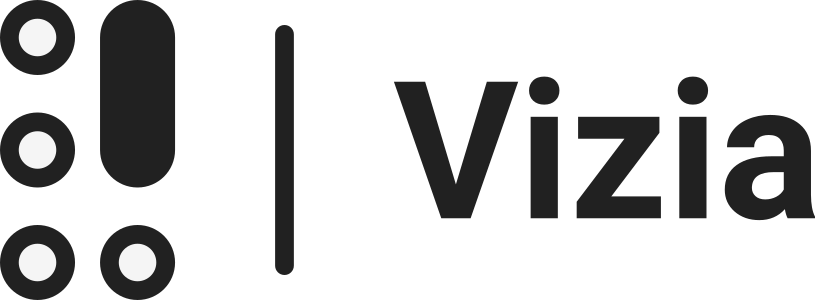
\includegraphics[scale=0.45]{img/logo_text_dark.png}
        \end{figure}
        {\Huge\bfseries%
            Glasses for the Visually Impaired \\[0.5em]
        }

        \vspace{10em}
        
        % Authors
        Prepared by: \\
        \vspace{1em}
        \begin{tabular}{cccc}
            Waleed Ahmed & Martin Ethier & Zain Denno & Connor Barker \\
            ECE & MME & ECE & ECE \\
            20659541 & 20660931 & 20654316 & 20711394 \\
            w29ahmed & methier & zdenno & cpbarker
        \end{tabular}
        
        \vspace{9em}
        April 12, 2022
    \end{center}
\end{titlingpage}
%% END TITLE

\newpage

\tableofcontents

\newpage

\section{Introduction}
\subsection{Problem Space}
The latest global estimates found that about 253 million people are visually impaired. Of those people, about 36 million are blind, meaning they have little to no vision \cite{orbis-global-blind-data}. Looking specifically at Canada and the United States, an estimated 1.5 million Canadians identify themselves as having sight loss \cite{cnib-blind-data}, and about 7.6 million Americans have a visual disability \cite{nfb-blind-data}. The Vision Loss Expert Group predicts that without increased access to eye health services, these numbers could potentially triple by 2050 \cite{orbis-global-blind-data}.

Taking a step back, it is worth investigating what being visually impaired or blind actually means. In one of our focus interviews, we were told by somebody who self-identified as blind that "Blindness is a spectrum". Very few people who identify as visually impaired or blind have no light perception at all. For most, blindness is a gradual degradation of sight. Some can see well, but only in certain light conditions. Others can only identify shapes or colours, and some have a field of vision so diverse and complex that is difficult to explain \cite{lighthouse-sf-info-page}. Another diverse aspect of blindness is when it is experienced in life. Some individuals are blind from birth, while others develop it at various points in life. While there are many causes of blindness, the leading ones are cataracts, age-related macular degeneration, glaucoma, diabetic retinopathy, corneal opacity, and trachoma \cite{WHO-blindness}.

Despite the diversity of conditions and visual impairment out there, there are many common problems faced by this demographic. One of the biggest ones, and one of the features of our project, is reading text. It doesn't occur to sighted individuals just how much text there is out in the world that contains crucial information we rely on to go about our day. Many visually impaired folk do not have this luxury and are missing out on key information that can help them to live more independently. While one solution to this is to ensure accompanying braille text wherever possible, there are still many situations where braille is not available. For example, text on a storefront or a postcard with your name and address on it to let you know the mail is for you. Other problems faced by the visually impaired community that our solution addresses are identifying colours and paper currency.

\subsection{Project Objective}
Extract, decode, and communicate information from an image to a visually impaired user through audio transcription.

\subsection{Key Terminology}
\setlength{\tabcolsep}{1em}
\begin{table}[ht]
    \centering
    \begin{tabular}{|p{5cm}|p{10cm}|}
        \hline
        Optical Character Recognition (OCR) & Broad term that describes any system that can extract and decode text from a digital representation such as an image or PDF \\ \hline
        iOS & Operating system used in Apple iPhones \\ \hline
        VoiceOver & Screen reader built into iOS \\ \hline
        Text-to-speech & Converting text to an audio transcription \\ \hline
        MFi Chip & Specialty chip needed for certain wireless capabilities when communicating with Apple devices \\ \hline
        System on a chip (SoC) & Integrated circuit that integrates the components of a computer \\ \hline
        Raspberry PI Zero W & Very small single-board computer with wireless capabilities \\ \hline
        CAD & Computer-aided design \\
        \hline
        API & Application programming interface \\
        \hline
    \end{tabular}
\end{table}

\section{Need Analysis Summary}
\label{need-analysis-summary}
The need analysis was carried out during the Spring 2021 term. Since we were satisfied with the results from this analysis, no further need analysis was conducted in Fall 2021 or Winter 2022. The section below is taken as-is from the Spring 2021 report.

\subsection{Problem Identification}
Since none of the group members are visually impaired, it was important to us to perform need analysis through speaking with individuals who are visually impaired or organizations that represent them. Doing this provided us with useful insight into some of the problems faced by the visually impaired, and allowed us to zero in on the features that would be the most useful to include in our design solution. Through our own research along with recommendations from our faculty advisor, Professor John Zelek, we identified a few organizations that advocate and aid the visually impaired that would be insightful to connect with. We were fortunate enough to hear back and have a chance to speak with a representative from Lighthouse SF and the University of Waterloo's AccessAbility Services.

\subsubsection{Interview with Lighthouse SF}
Lighthouse SF is an organization founded in 1902 and currently has headquarters in San Francisco, California. Their goal is to promote the independence, equality, and self-reliance of people who are blind or have low vision \cite{lighthouse-sf-homepage}. They pool together resources, hold seminars, and offer courses to help people with visual disabilities learn to use the latest and greatest assistive technologies. The individual that we had a chat with is currently an assistive technology instructor at the organization and self-identified herself as being blind.

During the interview, we discussed the various assistive technologies that exist and what her experience was with using them. She also enumerated a few very specific use cases where OCR technology currently does well, and where there is room for improvement. Some key takeaways were:

\begin{itemize}
    \item In the context of reading a physical book, one useful feature would be if the technology can automatically detect when the page has been turned and start reading out the next page without any additional explicit input from the user.
    \item There are two widely used "visual interpreter" apps called Be My Eyes and Aira. These apps connect the user with a sighted individual through a video call to assist in a task. The key difference between the two apps is that Be My Eyes works through sighted volunteers who lend their time for free and do not require any professional training, while Aira employs agents that are professionally trained visual interpreters to respond to calls.
    \item In the context of OCR, she mentioned that the most useful feature amongst other apps was the ability to instantly read out the text from a video feed, and in the cases where an image needs to be captured, audio-guided camera capture was useful. An example of audio-guided capture is when you are trying to get a picture of a document, all 4 corners of the document need to be visible for the image processing pipeline to extract out just the document from the image. One app, in particular, will say things like "left corner not visible" to inform the user why the captured image was not sufficient.
    \item One of the complaints about current OCR technology is that it does not perform well on handwritten text or non-standard machine fonts.
    \item She gave us a great quote: "Blindness is a spectrum" when we asked about the usability of wearable glasses. She mentioned that due to the diversity amongst visually impaired folks, some might know how to put on and use glasses due to losing their sight later in life, but it might not be as intuitive to someone who has been blind since birth.
    \item Another feature we asked her about is above the waist obstacle detection using computer vision. She mentioned that this is a feature that is not present in many solutions, but warned us that it is not as useful of a feature as we might think. It is only applicable in few scenarios, many individuals already use a white cane that is cheap and very capable for obstacle detection/avoidance in most scenarios.
    \item She informed us of a monthly meetup called Lighthouse Labs where engineers and developers working on assistive technology for low vision come to present their ideas. She extended an invite for us to attend and showcase what we end up building.
\end{itemize}

Overall, our biggest takeaway from the interview with Lighthouse SF was to double down on OCR as the primary feature of our design, as we spent the most time talking about it and we got the impression that it is the feature that is most useful. While we do have other additional features in mind, such as depth estimation, scene description, and money detection, we don't plan on spending any time on those until we feel confident our OCR works well.

\subsubsection{Interview with UW AccessAbility Services}
AccessAbility Services is responsible for working with students with disabilities to develop personalized academic accommodations at the University of Waterloo \cite{uw-accessability}. We spoke with a representative from the office who was employed as an adaptive educational technologist. There are 3 functional areas the office focuses on: class, assignments, and tests. Examples of potential services provided within the context of a visually impaired student for each of the functional areas are:
\begin{itemize}
    \item Class
    \begin{itemize}
        \item Reserved seating in a classroom if a student wishes to sit closer to the front or back
        \item Request professors to provide a transcript of lecture slides
        \item Request professor to allow student to audio or video record the lectures so that they can listen and transcribe them later on their own
        \item Note-taking services, such as asking for student volunteers to provide notes
        \item Get a textbook translated into braille or audio format
    \end{itemize}
    
    \item Assignments
    \begin{itemize}
        \item Asking for extensions to accommodate for additional difficulties of learning the content with a disability
    \end{itemize}
    
    \item Tests
    \begin{itemize}
        \item Getting students a scribe
        \item Requesting for oral tests instead of written tests
        \item Exams are done in special test centres where computers are setup that can read out the text for each question
        \item Get a test translated into braille
    \end{itemize}
\end{itemize}

In addition, a few technologies/products were mentioned that students had used in the past, including:
\begin{itemize}
    \item Jaws: Screen reading technology for the Windows operating system \cite{jaws-software}
    \item Kurzweil 3000: Educational software with text to speech features \cite{kurzweil}, not specifically tailored for visually impaired users though
    \item Read\&Write by TextHelp: A literary support tool that has useful OCR features in it \cite{read-and-write}. However, similar to Kurzweil, it's targeted at a general audience, in particular, grade school students
    \item Speechify: Mobile and desktop app for those with reading difficulties, low vision, and anybody interested in converting reading material to an audio format. Can read anything from the web, PDF, or images \cite{speechify}
\end{itemize}

There are even more assistive technologies available, and a more comprehensive list along with tutorials on how to use them are available on learn by self-registering for AccessAbility Services, which is available for every student, regardless of whether or not they are registered with a disability.

When asked what some of the complaints students had about existing technologies, we were told that screen reading technology often gets thrown off by weird formatting (captions, footnotes, etc.), and sometimes the voice reading it out can be a bit robotic. Speechify was highlighted as having realistic voices that are more pleasant and engaging to listen to.

Our key takeaway from this interview was an overview of some of the difficulties faced by visually impaired students in the context of academics. We were also pointed towards a lot of currently available products and technologies that are adjacent to our proposed design solution. Additionally, we mentioned if it would be possible for us to send out a survey or request to speak with visually impaired students to provide us with informal discussion/feedback on our design solution. We were told this is something that could be organized if we wish to proceed, and we plan on exploring this avenue later on in our design process in order to conduct some user studies and testing on our design.

\subsection{Survey of Available Products/Technologies}
Many products and solutions already exist in our chosen problem space. Reviewing them closely and identifying the pros and cons of each one allowed us to focus on the things that could be done better and potentially addressed by our solution. The five products we choose to focus on are Orcam MyEye 2, Envision, Seeing AI, Speechify, and Be My Eyes. Others exist, but these five are the closest and most relevant to our proposed design solution, so they are most valuable to examine.

\subsubsection{OrCam MyEye 2}
The OrCam MyEye 2 \cite{orcam} is a piece of hardware that can be attached magnetically to an existing pair of glasses. It is designed specifically for blind and visually impaired users and has a wide array of features to support that demographic. It can be controlled by voice or touch and can accomplish tasks such as read text, recognize faces, identify products, recognize barcodes, recognize money, and identify colours. Best of all, it can do all these features offline, meaning a network connection is not required. This means all of the processing is done right on the glasses. When we first identified the problem space and thought of potential solutions, something like the OrCam MyEye 2 is precisely what we originally had in mind. However, what we quickly realized with this product and others like it is that they are very expensive. Pricing information isn't readily available without consultation with OrCam, but we did find an article \cite{orcam-price} that mentioned \$3500 USD. Additionally, OrCam listed it on Amazon for \$5800 CAD \cite{orcam-amazon}. Even though the exact pricing isn't clear, it seems that the cost for this device is multiple thousands of dollars, which is very high. Globally, there are an estimated 200 million people who do not have access to assistive products for low vision \cite{WHO-assistive}. One of the reasons for this is products can be very expensive, and some individuals with a visual impairment may not have sufficient financial resources to purchase products with a premium price tag.

While the technology in this product is cutting edge and very useful, we feel that with some design changes, primarily offloading compute to a server or a user's phone, it should be possible to deliver a similar feature set at a much more accessible price point. After examining the OrCam MyEye, we identified cost as our primary constraint and focused on finding a solution that can minimize it.

\subsubsection{Envision}
Envision has two products, an app and a pair of glasses, targeted for the visually impaired \cite{envision}. The app can be used on its own without the glasses, and it uses the phone's camera instead of a camera attached to glasses. The app has features for reading text, scene description, colour detection, barcodes, and configurable object and people detection. The app initially comes with a one-week free trial, and then afterward runs on a subscription model. As of August 7th, 2021, the prices in CAD for the app are below:
\begin{center}
    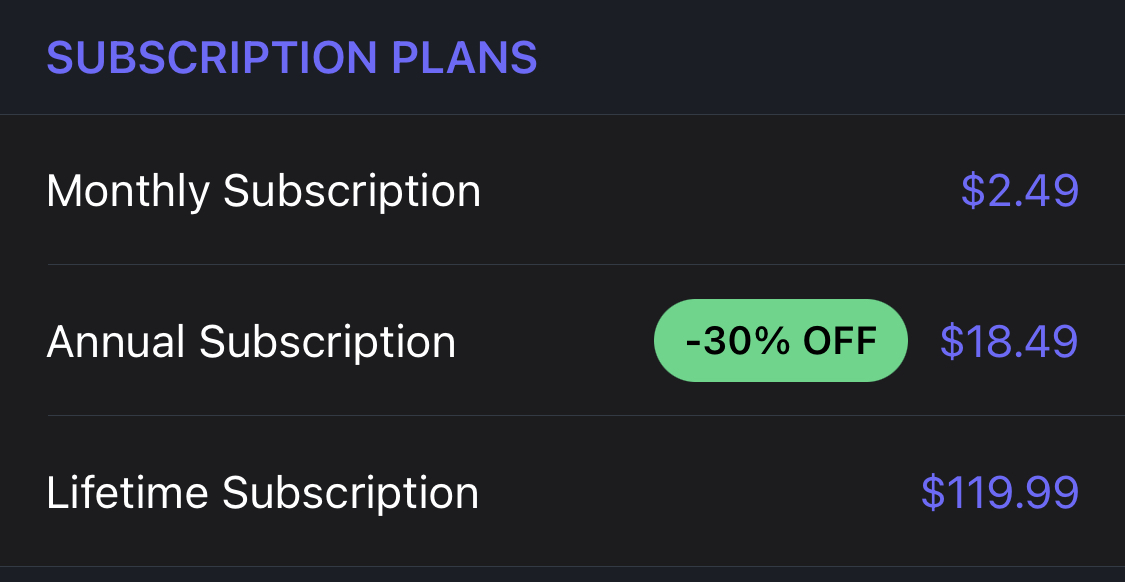
\includegraphics[width={0.7\linewidth}]{img/envision_app_price.jpeg}
\end{center}

Envision also has a pair of wearable glasses, built on top of the Google Glasses platform. All the features on the app are accessible with the glasses as well, as well as one additional feature that enables a video call that broadcasts a direct feed from the glasses. It is not clear from their website which of these features can run offline and which ones run online, as the glasses are capable of both wifi and Bluetooth. It's obvious that the video calling feature would require a network connection, but text detection could be done both offline or online. Additionally, the purchase of the glasses comes with a lifetime subscription to the accompanying application for both iOS and Android.

Similar to the OrCam MyEye, Envision is a great product with some cutting-edge features that are undeniably very useful for the visually impaired demographic. However, it suffers a similar problem in that it is very expensive. As of August 8th, 2021, the base model for Envision is listed as 3268.91 pounds, which is 5696.87 CAD.

\subsubsection{Seeing AI}
Seeing AI is a free application on iOS built as a part of Microsoft's "AI for Good" initiative \cite{seeing-ai}. Seeing AI has a lot of the same features that OrCam MyEye and Envision have, such as real-time short text detection, document reading, barcodes, face recognition, scene description, currency detection, and color detection. Two features that Seeing AI has that we couldn't confirm if MyEye or Envision have is handwritten text detection and light detection. Light detection is a unique feature that plays a sound that indicates how much light the camera detects. 

Some of these features work offline using on-device processing, while others utilize Microsoft's Azure cloud services and require a network connection. The features that require a network connection are document scanning, face detection, scene description, and handwritten text. The rest work offline.

The amazing part about this application is that it is totally free. There is no subscription or additional features available at a price. We found various other applications on the app store that would do a subset of features offered by Seeing AI, but they were not free. As a result, Seeing AI is considered the gold standard application for the visually impaired, as it is totally free and has a rich feature set. The individual we spoke to from Lighthouse SF was very familiar with this app and reported using it regularly.

After trying out this application, we really started to question if making a pair of glasses is even the way to go. If the end goal is to make it as cheap and accessible as possible, it's hard to compete with a free app that can do so much. The key insight that made us realize an affordable pair of glasses is still worthwhile to develop is the fact that it can be used without having to pull out and unlock your phone. Let's consider a specific example of wanting to read the name on a postcard. With Seeing AI, you'd have to pull out your phone, unlock it, find and open the Seeing AI app, switch to the "instant text" mode, and then have it read out the text for you. This might not seem so bad, but this process can be cumbersome for somebody who is visually impaired. However, with our solution, it would only require you to look towards the text you are trying to read, press a button on the glasses, and then after a small wait, the text will be read to you. This is fewer steps and allows you to more quickly read text out in the world. With this insight, we decided to continue pursuing our proposed design solution, even knowing now that a free alternative does exist.

\subsubsection{Speechify}
Speechify is a desktop and mobile app that can turn various forms of text into audio \cite{speechify}. The app is built on the premise that listening to something is easier and faster than reading it. It is not specifically for any demographic, but it can be used by anyone who has reading difficulty due to things like ADHD, Dyslexia, or visual impairment. Many people who have no problem reading still use Speechify, as it can increase productivity to get through large pieces of text faster by listening to it at faster speeds. Speechify can read anything on the internet, files, or images. It comes with a free option but there are paid features available, such as different voices that sound less robotic. This app was brought to our attention by UW AccessAbility services, as one of the complaints of many OCR technologies is the voice sounds very robotic, and Speechify was praised for having options for more realistic voices.

\subsubsection{Be My Eyes}
Be My Eyes is a free app that allows blind and visually impaired people to connect with sighted volunteers through a video call \cite{be-my-eyes}. This allows a sighted individual to assist in a task that a visually impaired person is having trouble with. Signing up to be a volunteer is free, and Connor has been a volunteer on the app for some time and has picked up three calls in the past. Waleed signed up for the app early in the term but has yet to get a notification to pick up a call. We examined this app as a way to potentially have interactions with visually impaired people, and get some insight into the kind of tasks that they need assistance with. An example use case would be for navigating an outdoor park. A visually impaired user may be in search of a bench to sit at and is not sure where to go. They can place a call for assistance on the app and a sighted volunteer will pick up and through the mobile phone's camera, guide the user to a nearby bench to sit at.

A notable mention is another app called Aira, which is built on the same premise as Be My Eyes, but instead of connecting visually impaired users with sighted volunteers, Aira employs trained visual interpreters who pick up the call.

Internally, we had some discussion about enabling a video call through the camera on the glasses, similar to the Envision glasses. This is not a high priority for us at the moment, but due to the success and usefulness of services such as Be My Eyes and Aira, it is something we are open to investigating further if time permits.

\subsubsection{Summary and Key Takeaways}
Assistive devices for the visually impaired is a problem space that has existed for quite some time, and as such, many solutions and products are currently available. Products like the OrCam MyEye 2, Envision, and Seeing AI offer a rich feature set and try to cover as many use cases as possible. The common feature, and the first one that each solution talks about, is the ability to detect and read text using OCR technology. It is reasonable to conclude that this is the most useful feature present in these solutions, and likely the one that gets the most usage. Therefore, we are choosing to focus on OCR as our primary feature, and only once we have that down will we start to consider some of the other features.

Additionally, due to the existence of Seeing AI, we plan on focusing our user experience around the glasses as much as possible. While we do want our app to eventually work without the glasses as well, and the user can simply use their phone's camera, it is less important to us since this functionality is already covered and implemented very well by Seeing AI. Our goal is to push this problem space forward with something that isn't too similar with what already exists.

\subsection{Patent Surveys}
The breadth of existing products with the same functionality as our solution has required us to carefully consider patent law when planning the design of our project. Specifically, OrCam owns a variety of patents protecting both their hardware and software products \cite{orcam-patents}. As the MyEye 2 is the device that most closely resembles our solution, we used their patent list as a starting point for our research. Other products, such as EnVision and NuEyes, possess IP as well, although these patents are either pending \cite{envision-patent} or unrelated to our solution.

Conveniently, the reason OrCam products are so expensive is also the reason we can successfully avoid patent infringement in our design. OrCam's patents are entirely related to proprietary software \cite{orcam-software} and hardware \cite{orcam-hardware}. Because we are using prefabricated hardware in the form of the Raspberry Pi and existing machine-learning software frameworks, neither of these components infringes upon OrCam's patents. OrCam does have some specific patents related to using a wearable camera in combination with machine learning software to drive an assistive device, although crucially these patents universally discuss performing machine learning on-platform. By offloading our machine-learning inference tasks to another device (the iPhone and servers), rather than using a dedicated processing device, our solution exists outside of the intellectual property patented by OrCam.

There is a possible issue of patent infringement concerning the doctrine of equivalents \cite{doctrine-of-equivalents}. This doctrine is a common legal rule which states that a device that does not literally fall within the realm of a patent may still be infringing upon said patent if it performs an identical function. This principle is often a legal grey area, and disputes regarding it are typically settled through a patent lawyer. While not experts, we believe that our solution avoids the doctrine of equivalents. While the system as a whole does perform a similar function to the OrCam MyEye 2, the subsystems involved do not. The wearable hardware's only purpose is to transmit an image wirelessly to either a server or a paired mobile app. In turn, the mobile application/server's only responsibility is to perform optical character recognition on an image. This image can be transmitted from an external source, or possibly captured by the smartphone camera. As a result, the solution performs an arguably different function entirely to OrCam's product. One of the qualifiers for the doctrine of equivalents to come into effect is that a "person skilled in the art" should consider the device or process equivalent to the patent being infringed upon \cite{doctrine-of-equivalents}. We feel confident that the novel addition of performing machine-learning on a mobile device and servers significantly differentiates our solution from OrCam's.


\section{Design Solution and Reformulation Summary}
Our design solution went through a few iterations as the terms went on. Sections \ref{winter-2021-design} - \ref{winter-2022-design} shows the system diagram in each term and highlights the key changes/reformulations for each iteration.

\subsection{Winter 2021}
\label{winter-2021-design}
\begin{figure}[H]
\centering
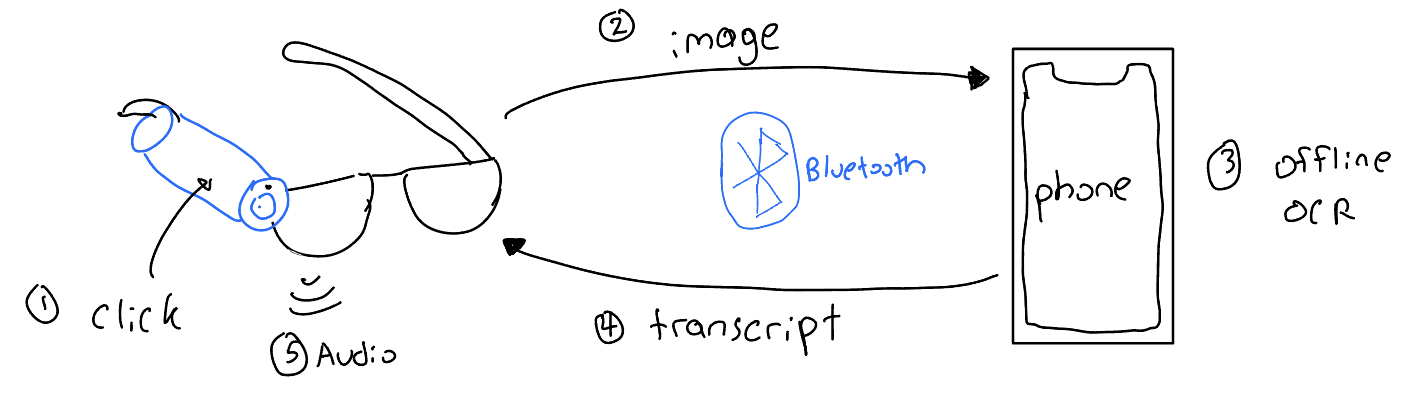
\includegraphics[scale=0.265]{img/system_diagrams/system_diagram_v1.jpeg}
\caption{System diagram v1}
\label{fig:system_diagram_v1}
\end{figure}
The winter 2021 term was prior to GENE 403 and was when we worked on our preliminary report to enroll in GENE 403. This term was spent brainstorming ideas and was when we decided the problem space we wanted to tackle was assistive devices for the visually impaired. Our initial conceptual design can be seen in Figure \ref{fig:system_diagram_v1}. The design was limited to only OCR at the time, and our primary goal was to build this solution without the need for a WiFi connection on both the glasses and iOS app, meaning it could work fully offline. The thinking was that if the phone has a strong enough chip, on-device processing would be sufficient for OCR, and we could communicate information between the glasses and iOS device using Bluetooth. Additionally, we had yet to decide at this point which text modalities our solution would support for OCR.

\subsection{Spring 2021}
\label{spirng-2021-design}
\begin{figure}[H]
\centering
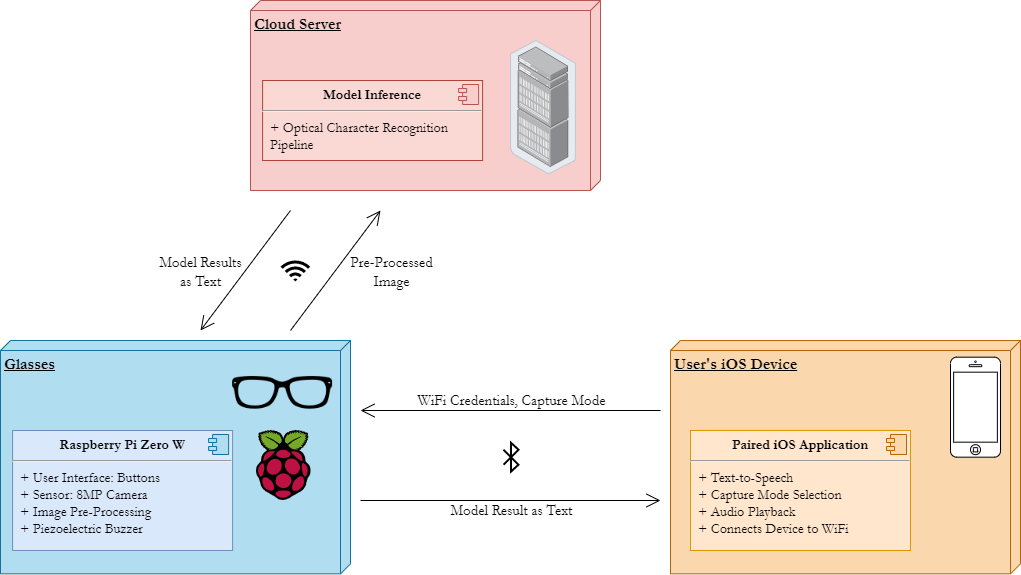
\includegraphics[scale=0.4]{img/system_diagrams/system_diagram_v2.png}
\caption{System diagram v2}
\label{fig:system_diagram_v2}
\end{figure}

The spring 2021 term was when Waleed, Zain, and Connor took GENE 403, and Martin was on a co-op term. The biggest change to our design this term was the introduction of a server to handle the OCR processing. The reason we decided to introduce a server is that we realized Bluetooth was not sufficient to send an image in a reasonable amount of time, at least not without Apple MFi certification. See sections \ref{bluetooth} and \ref{apple-mfi} for more on Bluetooth and Apple MFi. With the introduction of the server, a reliable WiFi connection is now required on the glasses to communicate with the server. 

At this point, we were still planning on using Bluetooth to communicate the OCR results from the glasses to the iOS device, which would perform speech synthesis and audio playback. The iOS device would also be responsible for forwarding WiFi credentials to the glasses, which would allow the glasses to configure the WiFi network on it's own.

A lot of OCR testing was done this term, using various libraries to try and determine which one would fit our needs best. Tesseract-OCR \cite{tesseract-github}, EasyOCR \cite{easy-ocr}, and PaddleOCR \cite{paddle-ocr} were tested, and we determined EasyOCR would fit our needs best since it provided good performance and looked the easiest to integrate with our solution. The three text modalities we wanted to support in our solution were text-in-the-wild, document text, and handwritten text.

The hardware platform for the glasses became more defined this term, as we decided a Raspberry Pi Zero W \cite{rpi-zero-w} would fit our needs, along with a 8 MP PiCamera \cite{rpi-camera}, buttons for interacting with the glasses, and a piezeoelectric buzzer for audio feedback to the user. The physical glasses design was yet to be finalized at this point, and our options were to either retrofit an existing pair of glasses with a clip-on solution, or make an entirely new pair of glasses specifically built for our platform.

\subsection{Fall 2021}
\label{fall-2021-design}
\begin{figure}[H]
\centering
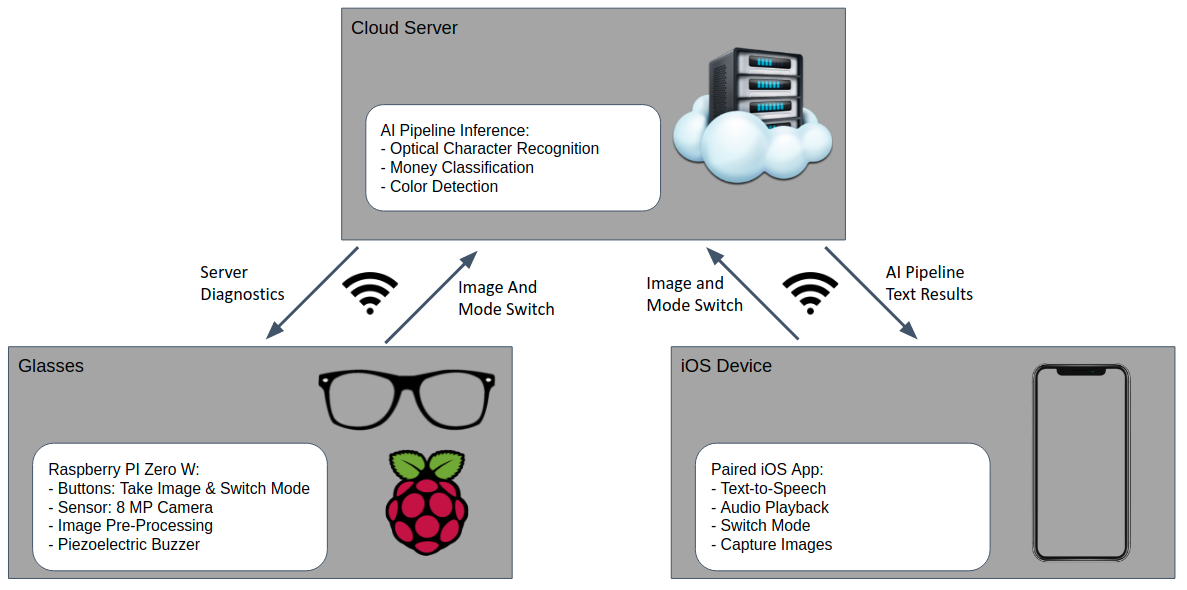
\includegraphics[scale=0.4]{img/system_diagrams/system_diagram_v3.png}
\caption{System design v3}
\label{fig:system_diagram_v3}
\end{figure}

In the fall 2021 term, Martin took GENE 403, while Waleed, Zain, and Connor were on co-op. Despite only one of us being in a school term, all of us still worked on the project and significant progress was made. One of the key changes to the system design was that the glasses and iOS device no longer communicate directly with each other. We realized that since we already introduced the requirement for the glasses to be connected to WiFi, we could propagate the same requirement to the iOS device as well, which allows the iOS device to now also be able to talk to the server. This is important because we wanted the iOS device to also be able to send images to the server and get results, meaning the app can function stand-alone without the glasses if this is desired. The server APIs are agnostic as to where the image comes from, so from its perspective, it doesn't matter if the image is coming from the glasses or the iOS device.

We tested another OCR library this term; Google Cloud Vision \cite{google-vision-api}, and found that it was even easier to use than EasyOCR, and the Google APIs also supported handwritten text, which is something EasyOCR did not perform as well on.

Most of the server code was written this term, and we also choose to introduce two new computer vision features: colour detection and money classification. We determined colour detection was straightforward enough to implement ourselves, see Section \ref{colour-detection} for an overview of our implementation. For money classification, we determined we needed to build a custom dataset of bills in real-world scenarios. We choose to support US bills since they do not have braille on them, which Canadian bills do have. We began building the money dataset and did some initial training on it as well, and the results looked encouraging.

The UI/UX for the iOS app was finalized, and a non-functional version of it was implemented. Simultaneously, some of the technical features; such as image capture, speech synthesis, and socket communication with the server to receive results, were developed in a separate test app. This way, once the UI/UX was ready, it would mostly be a matter of plugging in the functionality.

\subsection{Winter 2022}
\label{winter-2022-design}
\begin{figure}[H]
\centering
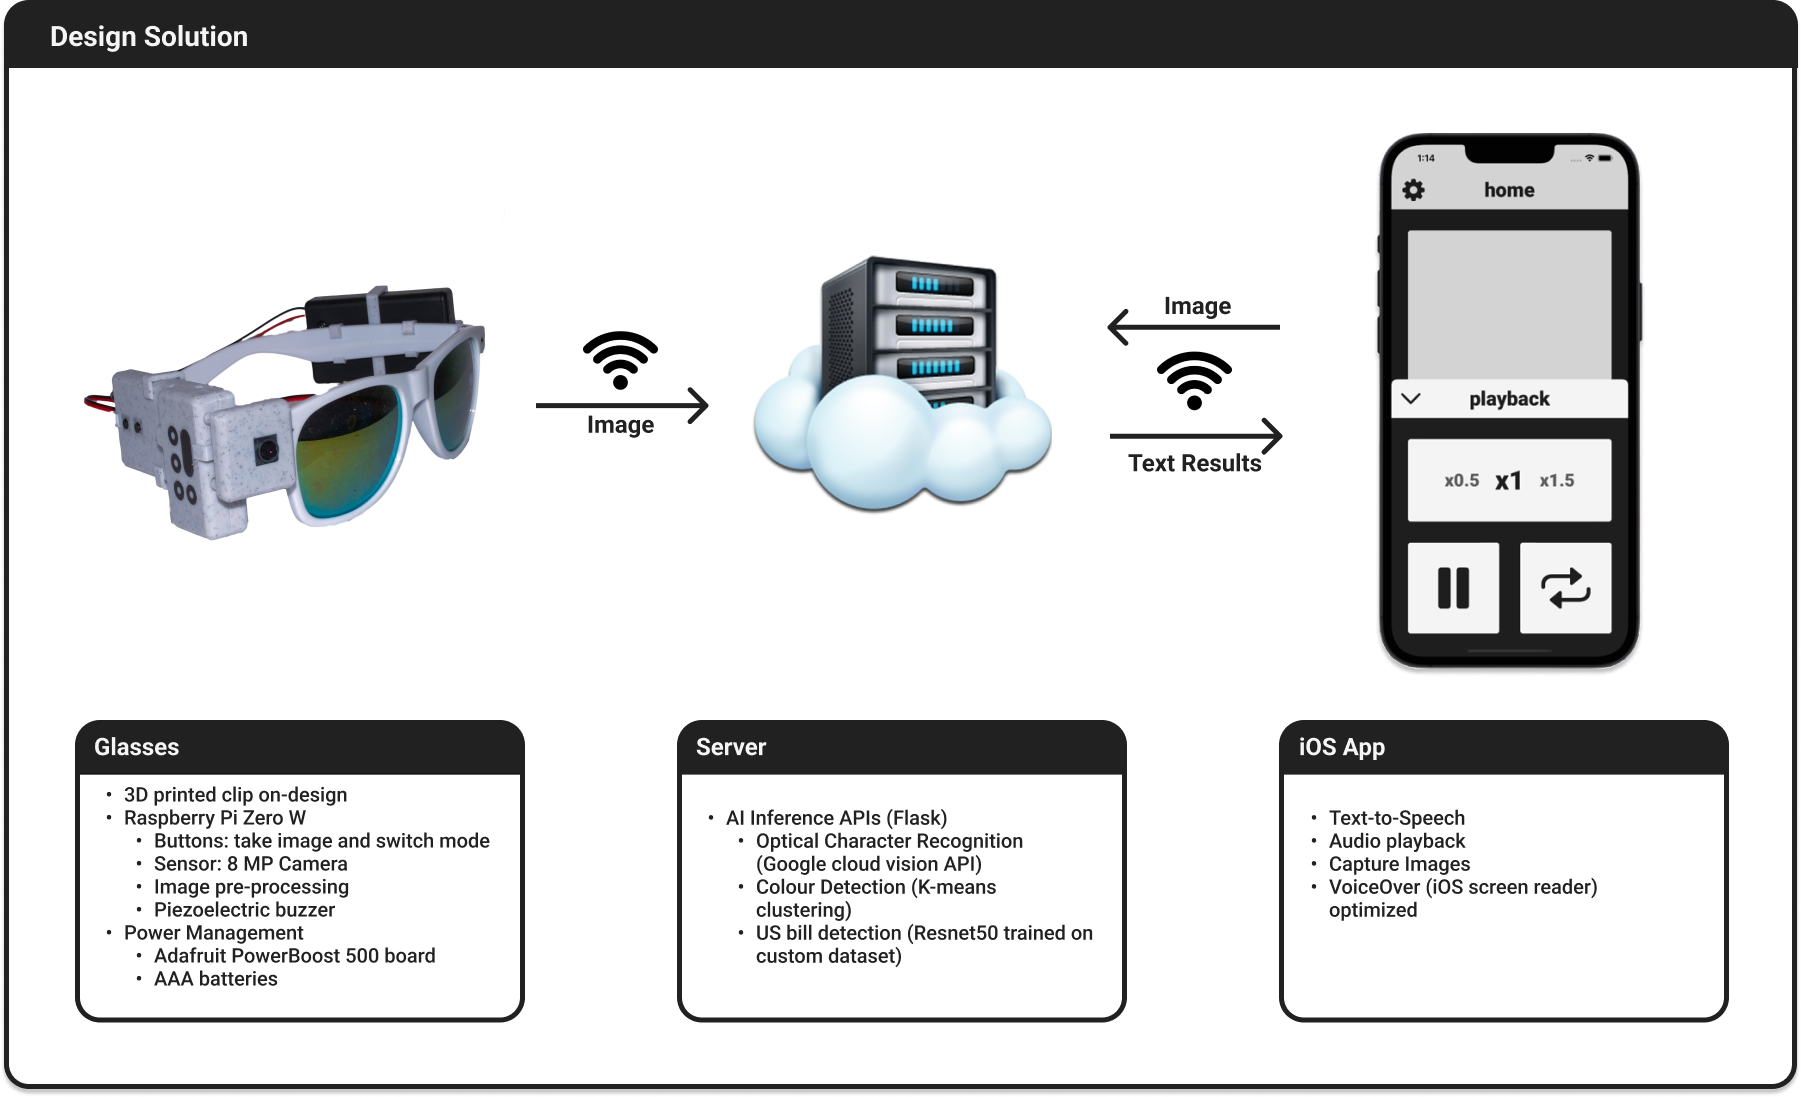
\includegraphics[scale=0.265]{img/system_diagrams/system_diagram_v4.png}
\caption{System design v4}
\label{fig:system_diagram_v4}
\end{figure}

In the winter 2022 term, all of our team members took GENE 404 together. At the beginning of this term, we had most of the functionality of our design implemented, and the goal was to polish it and integrate it all together. The main component of our solution that was yet to be designed was the glasses casing. We opted to go with a clip-on design, and all of the work to design, iterate, and integrate it with the glasses was carried out this term.

On the server, money classification was improved, by adding more images to the dataset, and also introducing a "no bill" class that would be used to identify when there was no bill in the image. The server code was polished and tested thoroughly as well to make sure everything worked well.

The UI/UX for the iOS app was mostly complete at the beginning of the term, and all of the functionality was brought into the app. Lots of integration testing was done between the app and the server, and then ultimately with the glasses as well once that was ready. One additional feature that was introduced to the app was multi-language speech synthesis. We noticed the Google Vision API would also return the language the text was detected in, and we forwarded this information to the app and used Apple's native speech synthesis libraries \cite{apple-speech-synthesis}, and to our surprise, it worked well out of the box for multiple languages. Before this term, we had only ever tried speech synthesis in English, but we tried out French, German, Spanish, and Arabic this term, all of which worked well.

\newpage
\section{Design Verification/Validation Summary}


\section{Design for Safety}

\section{Design for Regulatory Requirements}
Ontario (and the Canadian government), like many legal jurisdictions around the world, has regulations regarding the manufacture and sale of assistive devices. However, these regulations primarily impose restrictions upon medical technology. Our solution is non-intrusive and does not attempt or promise to perform a medical function of any kind. It, therefore, does not meet the requirements to be categorized as even a Class I medical device.

While our solution may not need to adhere to laws governing medically assistive devices, there are other regulations relating to data usage and privacy that must be carefully considered. The primary feature of the device is to read text to the user from a written or printed source, including medical paperwork, letters, and other sensitive or personal documentation. Data ownership in Canada is governed by an overlapping set of provincial and federal regulations, which apply differently to various use cases \cite{pipeda}. Our solution does not store any data, nor does it tie images taken by the user to them in any way. As such, the device is compliant with all relevant regulations.

\section{Impact on Society and Environment}
It is an unfortunate fact that despite increasing awareness and regulatory support, many disabilities are not accommodated in day-to-day life. This can force an individual with a disability to ask for help when performing a mundane task, or worse yet be unable to do it at all. In our preliminary analysis, we found that one of the universal needs of the disabled is independence. This is also the most significant way in which our solution impacts society at large.

The entire premise of our solution is increasing the independence of the blind or partially sighted when interacting with systems that are not designed to support accessibility (i.e. written materials without an accompanying braille translation). The solution is also designed to not be intrusive or obvious; almost all users of the product will have access to a pair of headphones, as iPhones come packaged with wired earbuds. The device is designed not to draw significant attention to the user, as smart glasses (while still not especially prevalent) are an established concept, and our product is functionally indistinguishable from them upon initial inspection. This low-profile, accessibility-improving solution fills an important niche for the blind or visually impaired when going about their lives with as much independence as possible.

As previously mentioned in our survey of available technologies, products that are functionally similar to our solution do exist. However, they are prohibitively expensive, particularly for disabled individuals who may be on a fixed income or have limited ability to work. The inexpensive nature of our solution makes it drastically more accessible to those who need it, increasing its potential to improve the independence of the disabled. It is our opinion that products designed to improve accessibility should adhere to that principle in all aspects of their design, including affordability for the groups they target.

Furthermore, we intend to make the entire platform (software, hardware, accompanying instructions) fully open-source. We firmly believe that the benefits of making the solution publicly available far outweigh any downsides related to losing profit should our project become a fully-fledged product. Not only does this make the product even more inclusive to those on a limited budget, but it provides the opportunity for technologically-minded individuals who are blind or partially sighted to contribute valuable new ideas and features we may not have considered. This has the added benefit of increasing the independence of the community as a whole; rather than needing to rely on general-purpose products which may not perfectly suit the requirements of an individual, open-sourcing the project means that a user can easily modify their own system, or build a new one based on our design.

Finally, we chose to print the housing out of PLA, a cornstarch-based bioplastic. This material releases no harmful fumes when used for 3D printing, from either a health or environment standpoint. This material strikes a balance between durability and biodegradability, but it is able to be composted in an industrial environment (i.e. under higher temperatures, with the aid of microbial digestion). The main environmental benefit of using PLA is that no crude oil is used in its production; only corn. It is also one of the cheapest and easiest to use materials for 3D printing, making it an ideal candidate for a cheap, widely-available option for printing our open-source design.

\section{Design Project Management Summary}

\section{Conclusions and Recommendations for Future Work}

\section{Acknowledgements}
https://www.overleaf.com/project/6245c3ce4f2a564aea8bd3c6
\newpage
\section{Appendix A - Design Solution Description}
\subsection{System Level Representation}

\begin{figure}[H]
\centering
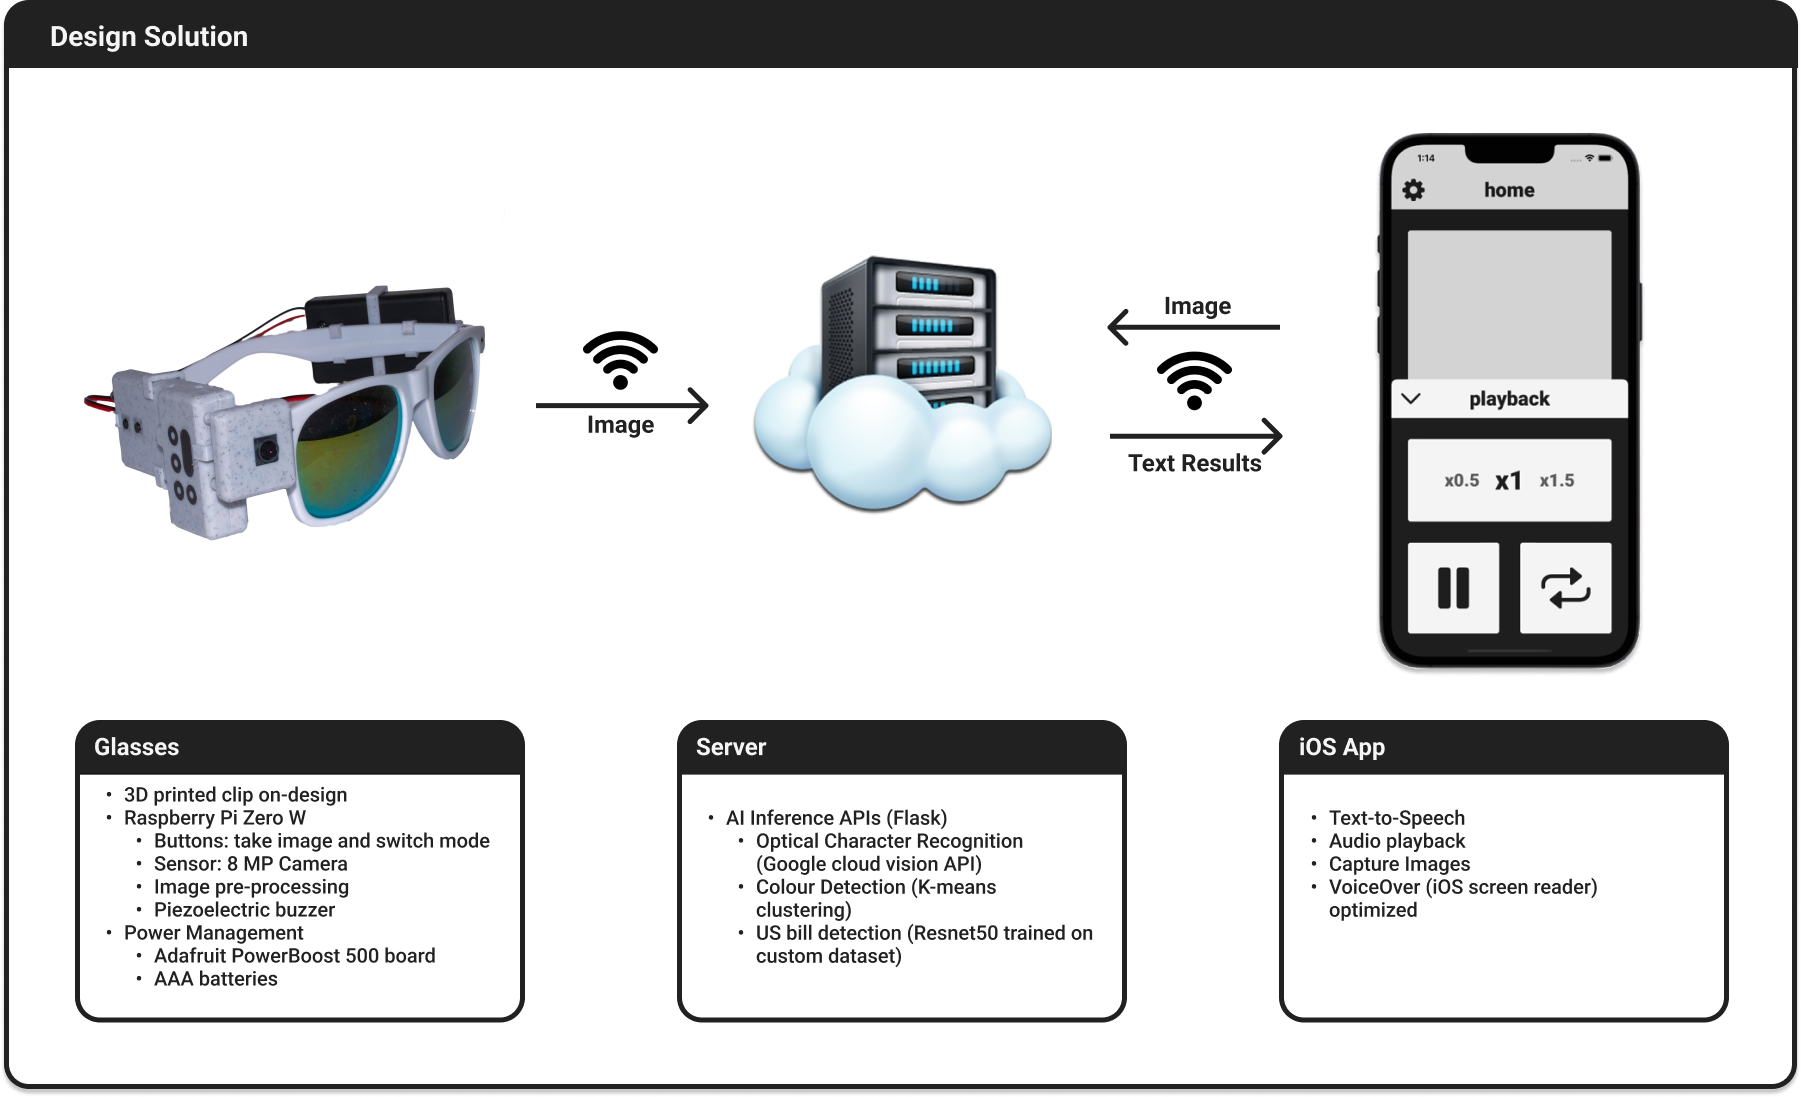
\includegraphics[scale=0.265]{img/system_diagrams/system_diagram_v4.png}
\caption{System design diagram}
\label{fig:system_diagram}
\end{figure}

Our design consists of 3 components: glasses, a server, and an iOS application. Figure \ref{fig:system_diagram} shows how these components interact with each other. The glasses send an image to the server, the server processes the image, and then the results are sent to the iOS app to be presented to the user through audio. The app is also capable of taking images and sending them to the server, and this allows the app to be used without the glasses.

Our original vision for this project was to avoid the need for an internet connection on the glasses and iOS device. Our goal was to do all of the computer vision processing on the iOS device and communicate information between the glasses and the iOS device using Bluetooth. However, we discovered Bluetooth limitations that make it impractical to reliably and quickly send an image over Bluetooth. See sections \ref{bluetooth} and \ref{apple-mfi} for more details.

\newpage
\subsection{Glasses}
\begin{center}
    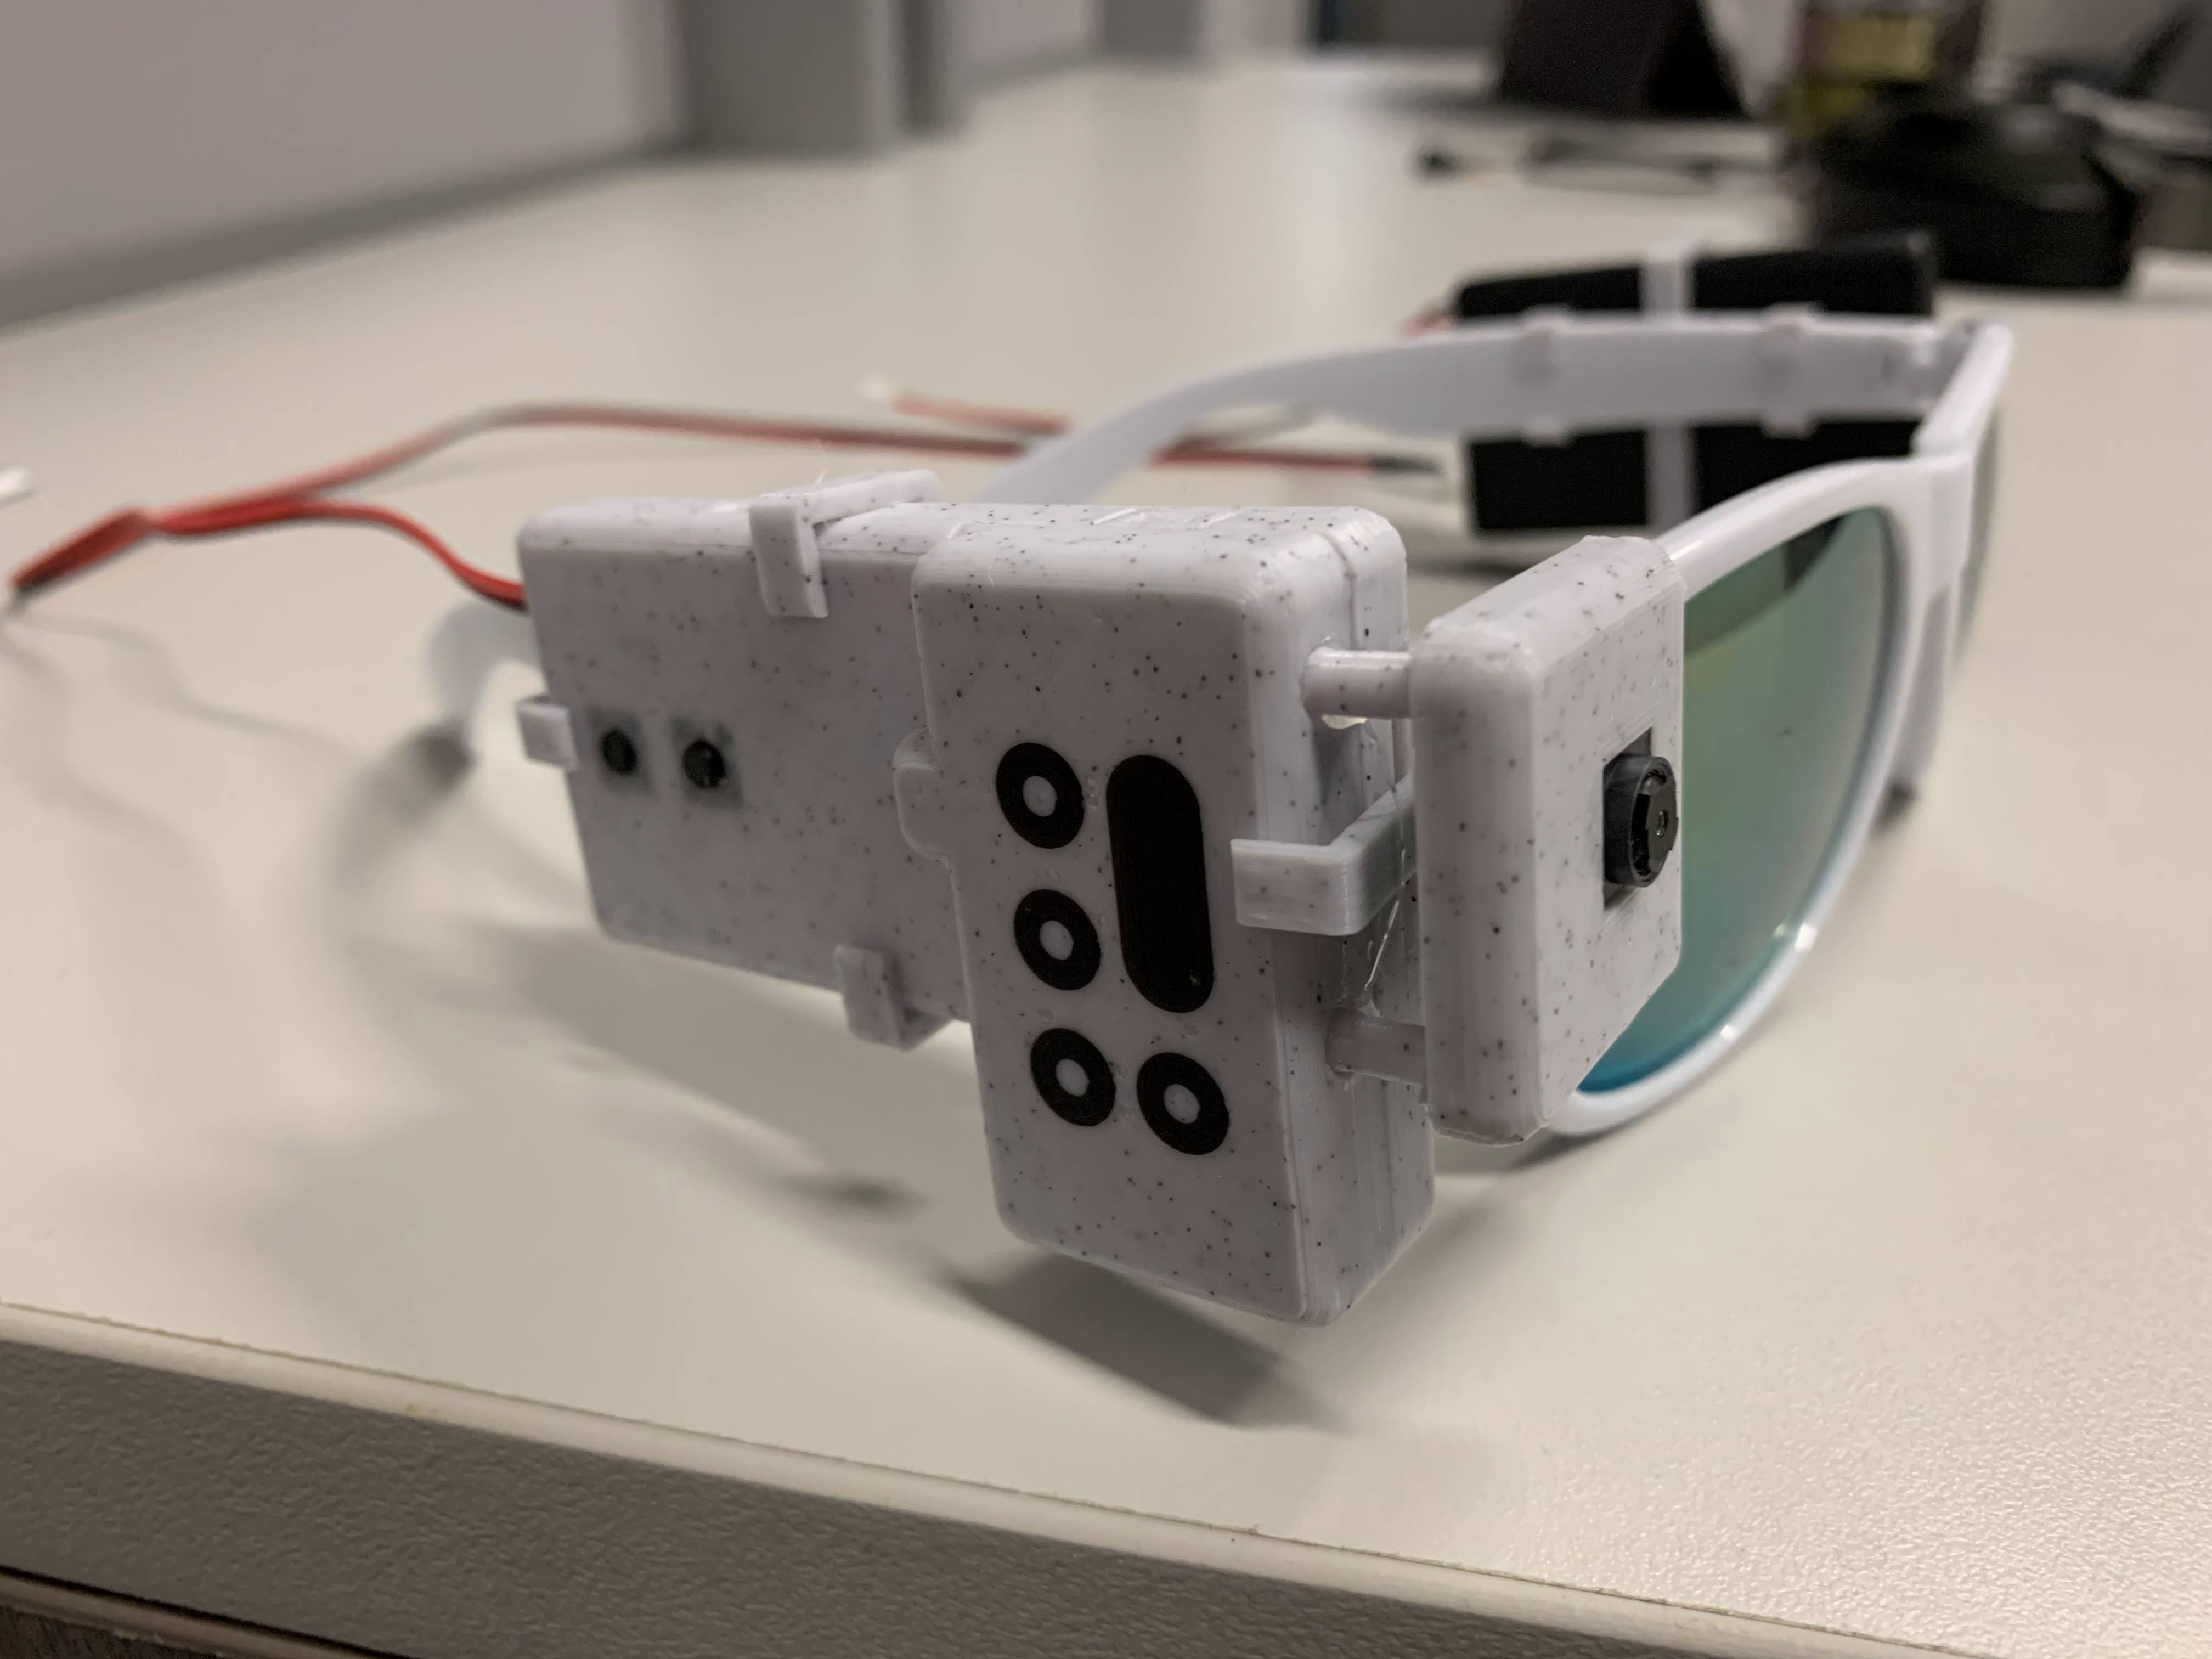
\includegraphics[width={0.3\linewidth}]{img/glasses/left.jpg}
    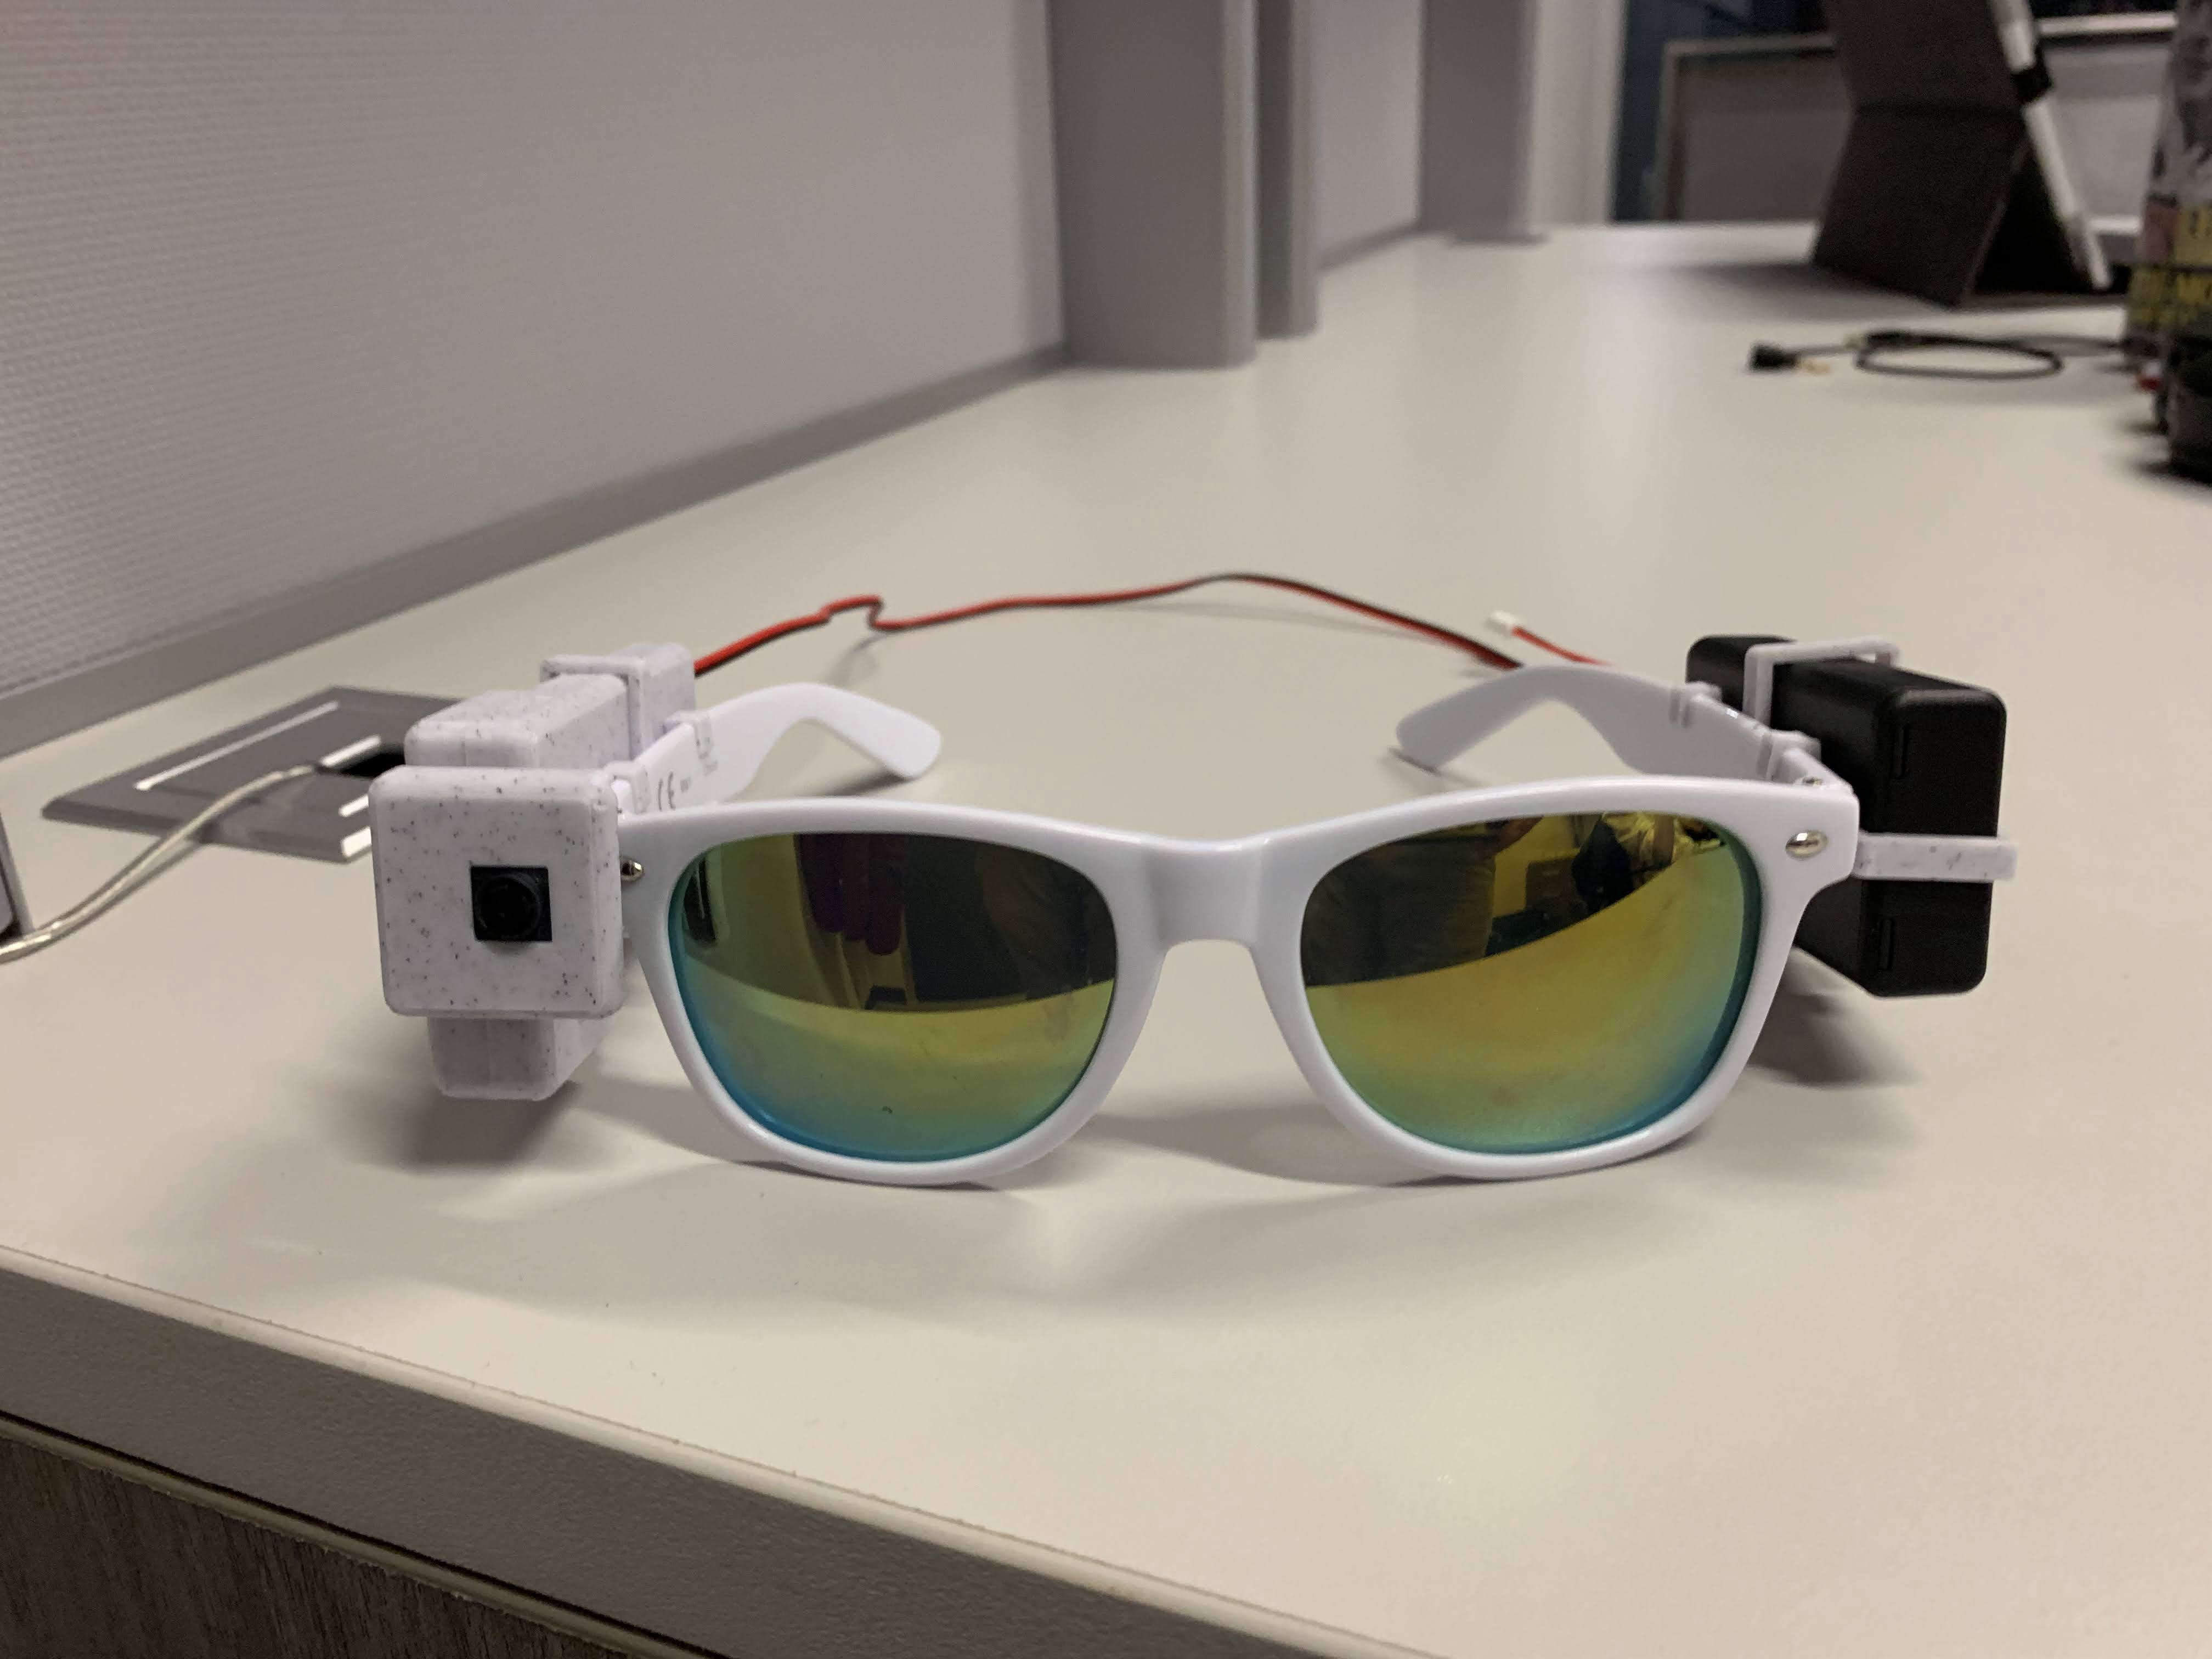
\includegraphics[width={0.3\linewidth}]{img/glasses/middle.jpg}
    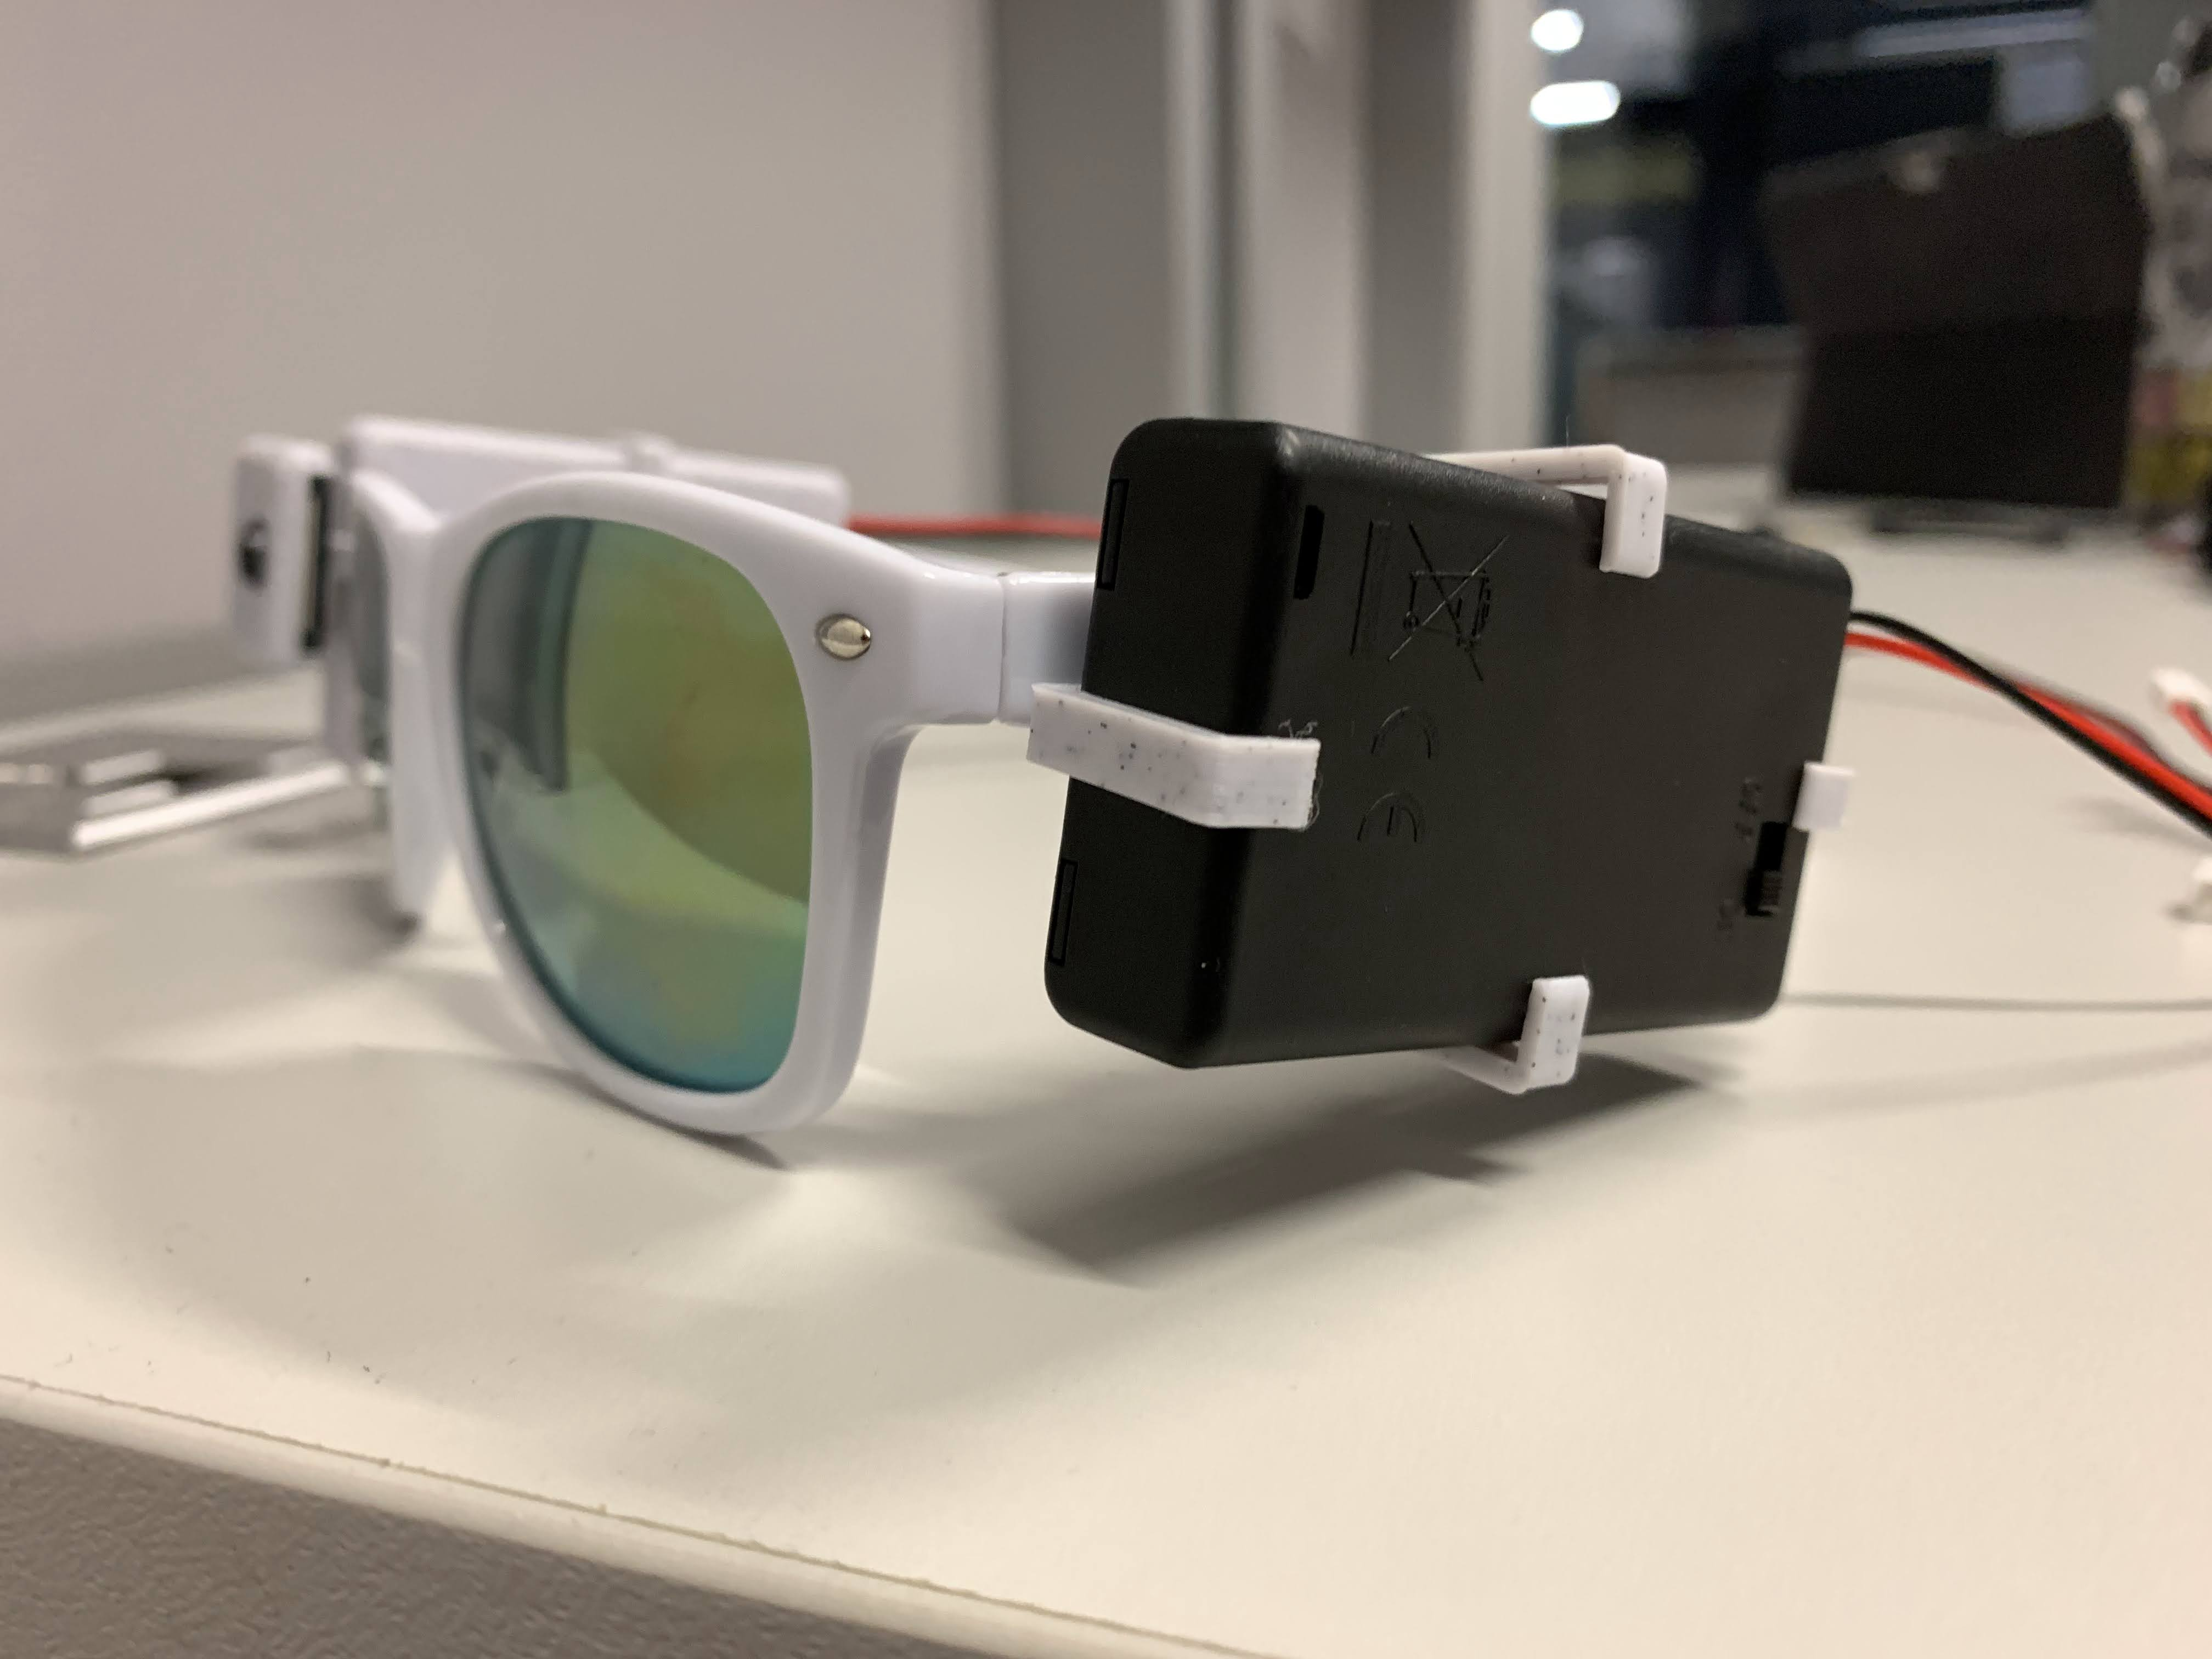
\includegraphics[width={0.3\linewidth}]{img/glasses/right.jpg}
\end{center}

A 3D printed clip-on design was used to allow flexibility since it can be attached to any pair of glasses. There are two pieces that attach to the glasses, the module on the right side is the compute unit, storing a Raspberry Pi Zero W, Adafruit PowerBoost 500, 8 MP Camera, 2 buttons, and a piezoelectric buzzer. The Raspberry Pi is responsible for all of the compute and managing the GPIO, the PowerBoost board is for power management, one button is to take a picture, another is to switch between different processing modes, and the piezoelectric buzzer is to communicate any errors or low battery warnings. The module on the left side is the power supply, which is a battery holder for 3 AAA batteries. There is a wire that goes between the 2 modules to connect the power supply, and this wire also doubles as a holder for the glasses in case the user wants to take it off their face and keep it around their neck. The great thing about this design is that the total cost of parts is less than 200 Canadian dollars, and the STL files are provided by us so anybody can print the clip-on design using a 3D printer.

\subsubsection{Housing Design and Fabrication}
The housing for the glasses was designed from scratch using CAD software. The main goal of the housing was to be lightweight and compact, which was mostly a matter of measuring, test fitting, and repeating until the case was as tightly fit as possible. Most of the difficulty in designing the housing came from the challenge of designing a case that could be 3D printed using the minimum amount of support structures possible, as well as being able to be easily assembled and disassembled (ideally without glue). The housing also needed to function agnostic of the specific pair of glasses being used, meaning the mounting solution couldn't be integrated.

The ultimate solution for the glasses was to print the case in three pieces, which attached to one another with integrated clips. Each part of the housing is printed facing downwards, i.e. with the flat side against the build plate. This allows for minimal use of support structures, resulting in a much faster print time, lower material usage, and high durability. Via the use of internal standoffs, the electronics are held in place inside the case without glue (while also being aligned with openings for cables/buttons/etc). Both the battery pack and electronics housing use a wrap-around clip system which holds itself together, meaning no glue is needed to assemble them. These clip harnesses attach to the glasses arms using 2 small clips; in order to size the system to their glasses, a user only needs to measure one arm of their glasses at two points, and then print all 4 small clips. The material cost of the case is around \$0.30, and the total print time is approximately 2h.

\subsection{Server}
\label{server}
The server is where all of the computer vision processing happens, and the results of the computation are sent back as a response and it can also be emitted on a socket, which the iOS app listens on so that it can receive the results in the event that the image was sent from the glasses. There are 3 features supported by the server: optical character recognition (OCR), colour detection, and money classification. The server is implemented in Flask, a micro web framework written in Python, and it was chosen since our computer vision code is implemented in Python, so having the server code in the same language makes it easier. There are 4 APIs exposed by the server:

\begin{itemize}
    \item \texttt{/ocr}: Performs optical character recognition.
    \item \texttt{/detect\_color}: Finds the top k colours in an image, with k being configurable.
    \item \texttt{/classify\_money}: Looks for all denominations of US bills. Also specifies when no bill is found in the image.
    \item \texttt{/socket\_emit}: Emits any string on a socket path. Used to communicate state changes from the glasses to the iOS app.
\end{itemize}

\subsubsection{Optical Character Recognition (OCR)}
Optical Character Recognition is generally a difficult task for computer vision systems. There are currently many existing solutions available to perform OCR. During the Spring 2021 term, different OCR libraries were tested and the best library was selected to be used in the project. Please refer to our Spring 2021 report for the details of the testing. In summary, we tested EasyOCR \cite{easy-ocr}, PaddleOCR \cite{paddle-ocr}, Tesseract-OCR \cite{tesseract-github}, and the Google Cloud Vision API \cite{google-vision-api}, and found that the Google Cloud Vision API offered the best performance and the most features. This term, we further tested the Google Cloud Vision API and became more confident in its performance and capabilities. One new feature we incorporated was language-specific text synthesis. We noticed the results from the Google API returned a language code for the text it finds, and we are able to forward this language code to the iOS app's speech synthesizer, and this way, it will speak the text in the locale of the language it is detected in. Google Cloud vision API currently supports 60 languages \cite{google-languages}, and while we didn't verify every single of them, we tried a subset of them with our iOS speech synthesis and it appeared to work well. Additionally, the Google vision API supports all three of our target modalities: text-in-the-wild, documents, and handwritten. See figure \ref{fig:google_vision_examples} below for example output from the Google APIs.

\begin{figure}[H]
\centering
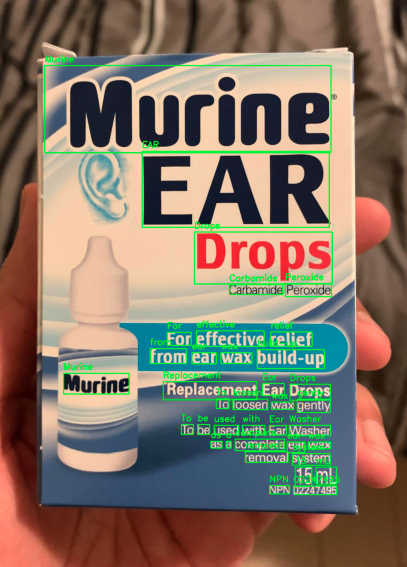
\includegraphics[scale=0.5]{img/cv/ocr/ocr_text_in_the_wild.png}
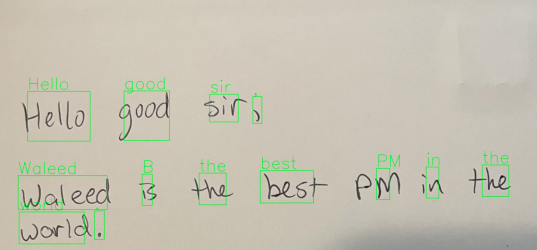
\includegraphics[scale=0.5]{img/cv/ocr/ocr_handwriting.png}
\caption{Examples of results from Google Cloud Vision API}
\label{fig:google_vision_examples}
\end{figure}

\subsubsection{Colour Detection}
\label{colour-detection}
Colour detection refers to identifying the most prevalent colours in an image. We got the idea to implement this since the feature exists in Seeing AI, and the individual we spoke with from Lighthouse SF mentioned she used this feature often to identify the colours of clothing, in order to decide what outfit to wear. We determined this would be a relatively straightforward algorithm to implement so we did it ourselves. Since the end goal is to report colours by name, and not the pixel values, we needed a database of colours with their associated RGB values to use as a reference. We used three such databases, which we referred to as small, medium, large, and they can be found
\href{https://github.com/vizia-fydp/server/tree/main/color_detection}{\color{blue}{here}}
 in our server repository. The small and medium databases are from \cite{color-small-medium}, and the large one is from \cite{color-large}. The small, medium and large databases have 17, 140, and 866 colours respectively. Note that we included HSV pixels for each colour as well as that is something we wanted to experiment with.

To implement this feature, we came up with two algorithms, described below:

\newpage
\begin{enumerate}
    \item For each pixel, find the euclidean distance to each colour in the database. The colour with the smallest euclidean distance is chosen as the best match for this pixel. Keep a count of which colours appear, and sort it by count, from highest to lowest count. Pick off the top K colours from this count.
    \item If K colours are desired, performs K-Means Clustering \cite{k-means-wikipedia, k-means-opencv} with 2*K clusters, pick out the top K clusters and calculate euclidean distance between the cluster mean and all colours in the database. Pick the colour from the database with the smallest euclidean distance as the match for that cluster.
\end{enumerate}

The equation for the euclidean distance can be seen in Equation \ref{eq:euclidean_dist}, where $d_i$ is the distance to the $i_{th}$ colour in the database. 

\begin{equation}
\label{eq:euclidean_dist}
d_i=\sqrt{(R - R_i)^2 + (G - G_i)^2 + (B - B_i)^2}
\end{equation}

Both algorithms were implemented and tested, and found that they produced similar results. However, algorithm 2 ran a little bit faster, even with optimizations made to algorithm 1. We kept code for both algorithms in the server code, but algorithm 2 is used due to its lower computational cost.

We choose to set K=3 to report the top 3 colours in the image as that seemed most appropriate, however, this parameter is easily configurable since the \texttt{/detect\_color} API takes K as an argument.

Figures \ref{fig:color-detection-output-1} - \ref{fig:color-detection-output-4} shows output of algorithm 2 using all three color databases, 6 k-means clusters, and the top 3 colour names.

\begin{figure}[H]
\centering
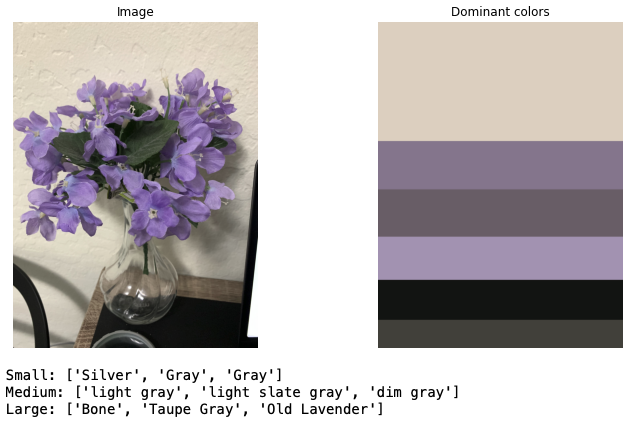
\includegraphics[scale=0.6]{img/cv/colour_detection/colour_detection_1.png}
\caption{Colour detection output}
\label{fig:color-detection-output-1}
\end{figure}

\begin{figure}[H]
\centering
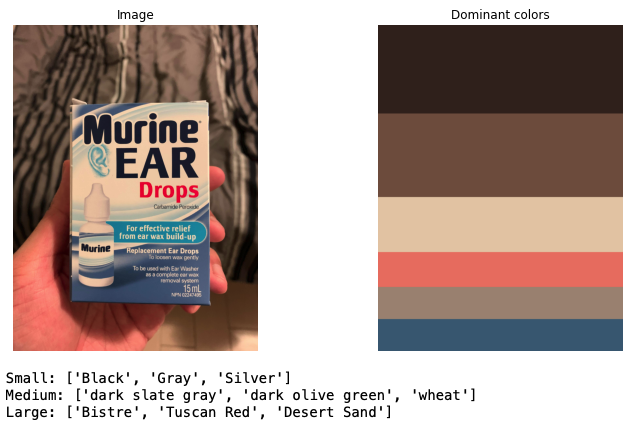
\includegraphics[scale=0.6]{img/cv/colour_detection/colour_detection_2.png}
\caption{Colour detection output}
\label{fig:color-detection-output-2}
\end{figure}

\begin{figure}[H]
\centering
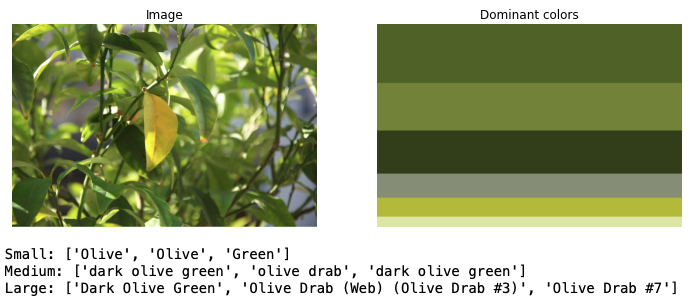
\includegraphics[scale=0.6]{img/cv/colour_detection/colour_detection_3.png}
\caption{Colour detection output}
\label{fig:color-detection-output-3}
\end{figure}


\begin{figure}[H]
\centering
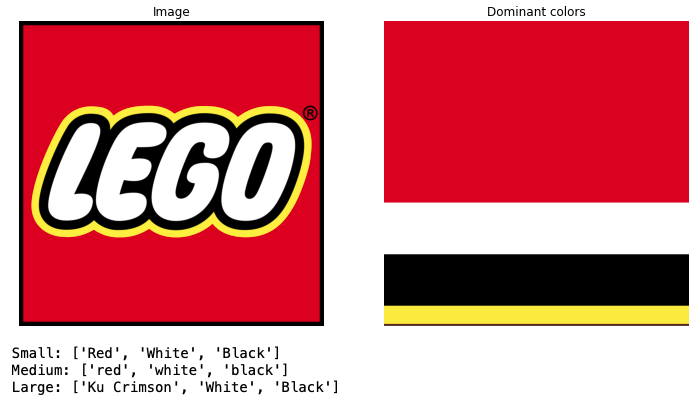
\includegraphics[scale=0.6]{img/cv/colour_detection/colour_detection_4.png}
\caption{Colour detection output}
\label{fig:color-detection-output-4}
\end{figure}

The small database isn't descriptive enough, the medium database has trouble with some real-world images, particularly in poor lighting conditions, and the large database is a little too descriptive, some of the colours sound confusing even to sighted individuals. We ended up choosing the medium database to use in production, as it works well as long as the lighting conditions are acceptable, so we can suggest to the user to use the flash on the phone when taking images.


\subsubsection{Money Classification}

Money classification is the task of identifying the type of bill being shown in the image. We targeted American bills only for this task since Canadian bills have braille on them to identify the bill type. After some research, we could not find any open-source money classification algorithms already existing. Therefore, we decided to implement our own classification algorithm.

It was decided early on that a convolutional neural network (CNN) would be a good fit for this task, since these types of networks are typically very good at classifying object based on visual patterns. The first step to having a CNN classify bills is building a dataset. To build this dataset, members of the group acquired American bills and took photos of them in various situations and orientations using their phones. The photos were saved in a folder on Google Drive and the images were separated into sub-folders, each corresponding to the type of bill. The preliminary version of the dataset was collected in the Fall 2021 term, where we collected a total of 405 images for the dataset, corresponding to the bill types of 1, 5, 10, 20, and 50 dollar bills. At the start of the Winter 2022 term, we decided to collect more images for each bill class to increase robustness and also added images corresponding to 100 dollar bills. We also realized that we needed a "no bill" class, since the model was just predicting one of the bill classes even when there was not a bill present in the image. To collect images for this class, we simply collected images around our homes of random objects without any bills in the image. Our final dataset version had 706 total images belonging to 1, 5, 10, 20, 50, 100, and "no bill" classes. When collecting the bill images for the dataset, we tried collecting images of the bills in as many situations as possible, to ensure robustness in our classifier. Some of the possible situations we thought of are:

\begin{enumerate}
    \item Bill in center of image vs. bill closer to edge of image
    \item Nice bill vs. bill with edges folded vs. crumpled bill
    \item Holding bill in hand vs. bill resting on table/chair/floor
    \item Indoors vs. outdoors
    \item Good lighting vs. bad lighting
    \item Front side of bill vs. back side of bill
    \item Bill upside down
    \item Bill rotated
\end{enumerate}

Some example images from the dataset can be seen in Figures \ref{fig:one_dollar_nice} and \ref{fig:one_dollar_hard}. In the first image, we can see an example of a relatively easy bill to classify. In the second image, this is clearly a more difficult problem due to the bill being folded multiple times.

\begin{figure}[H]
\centering
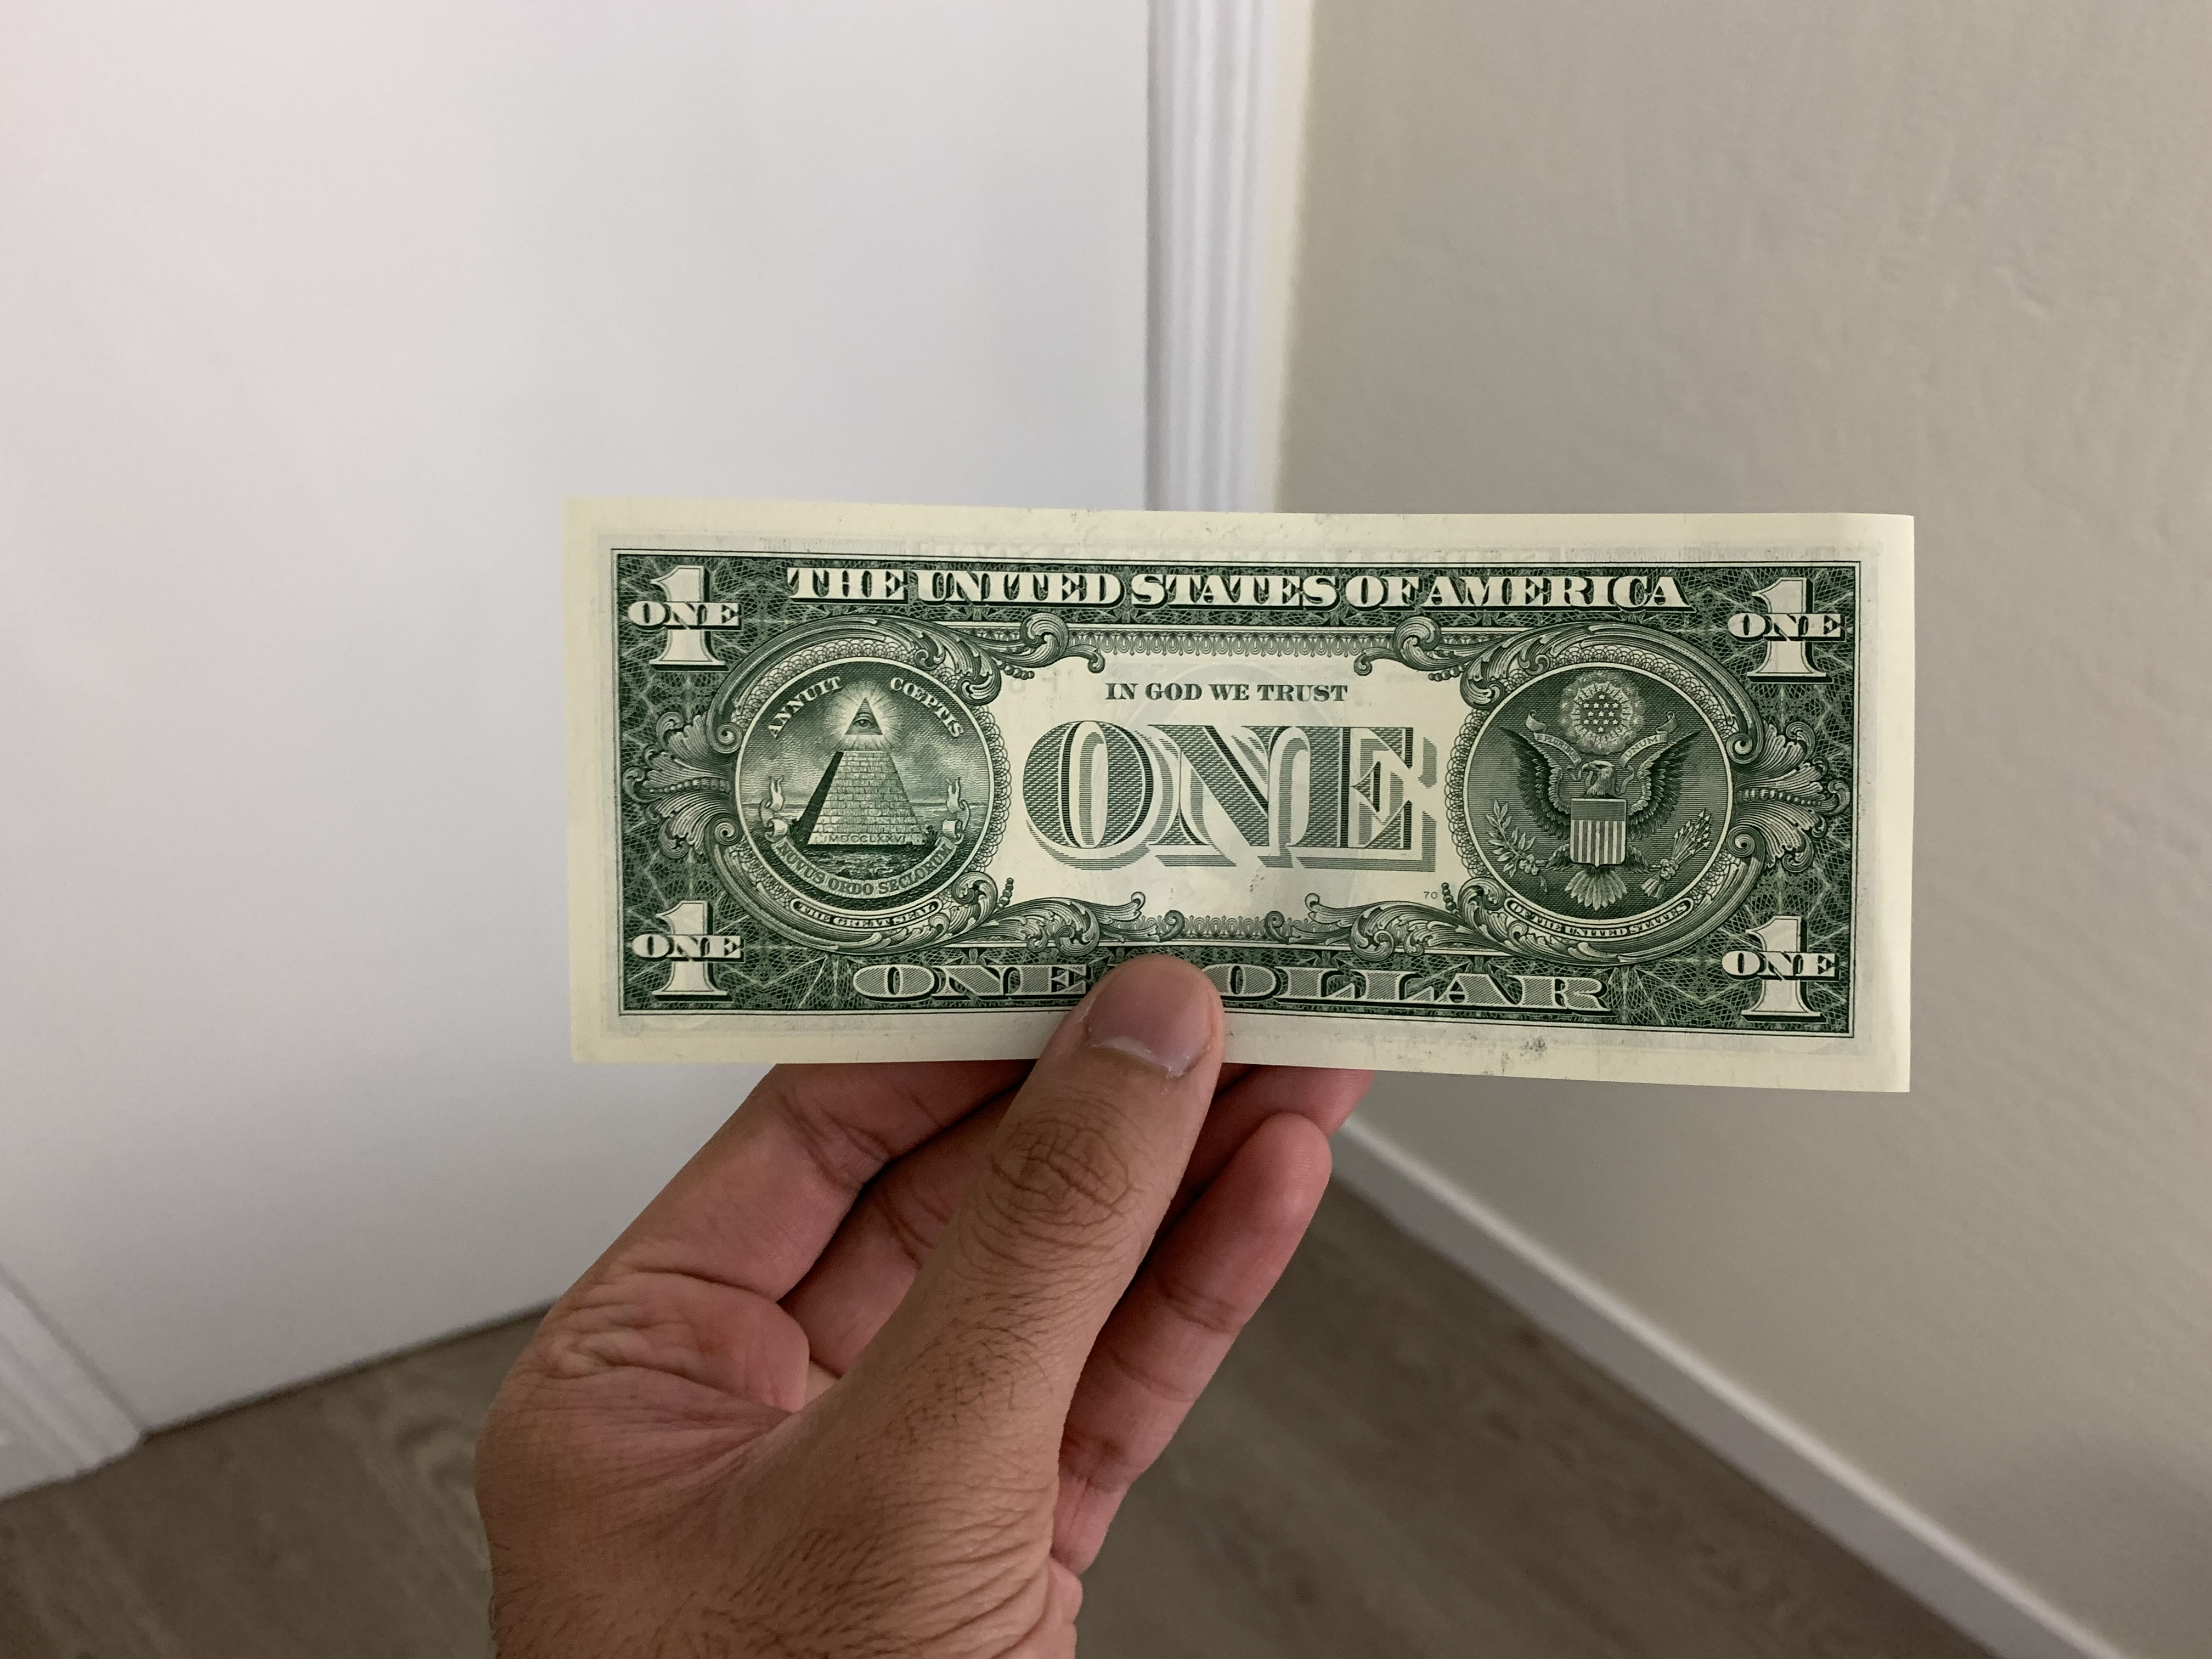
\includegraphics[scale=0.1]{img/cv/money/one_dollar_bill_nice.jpeg}
\caption{Easy example of a one dollar bill.}
\label{fig:one_dollar_nice}
\end{figure}

\begin{figure}[H]
\centering
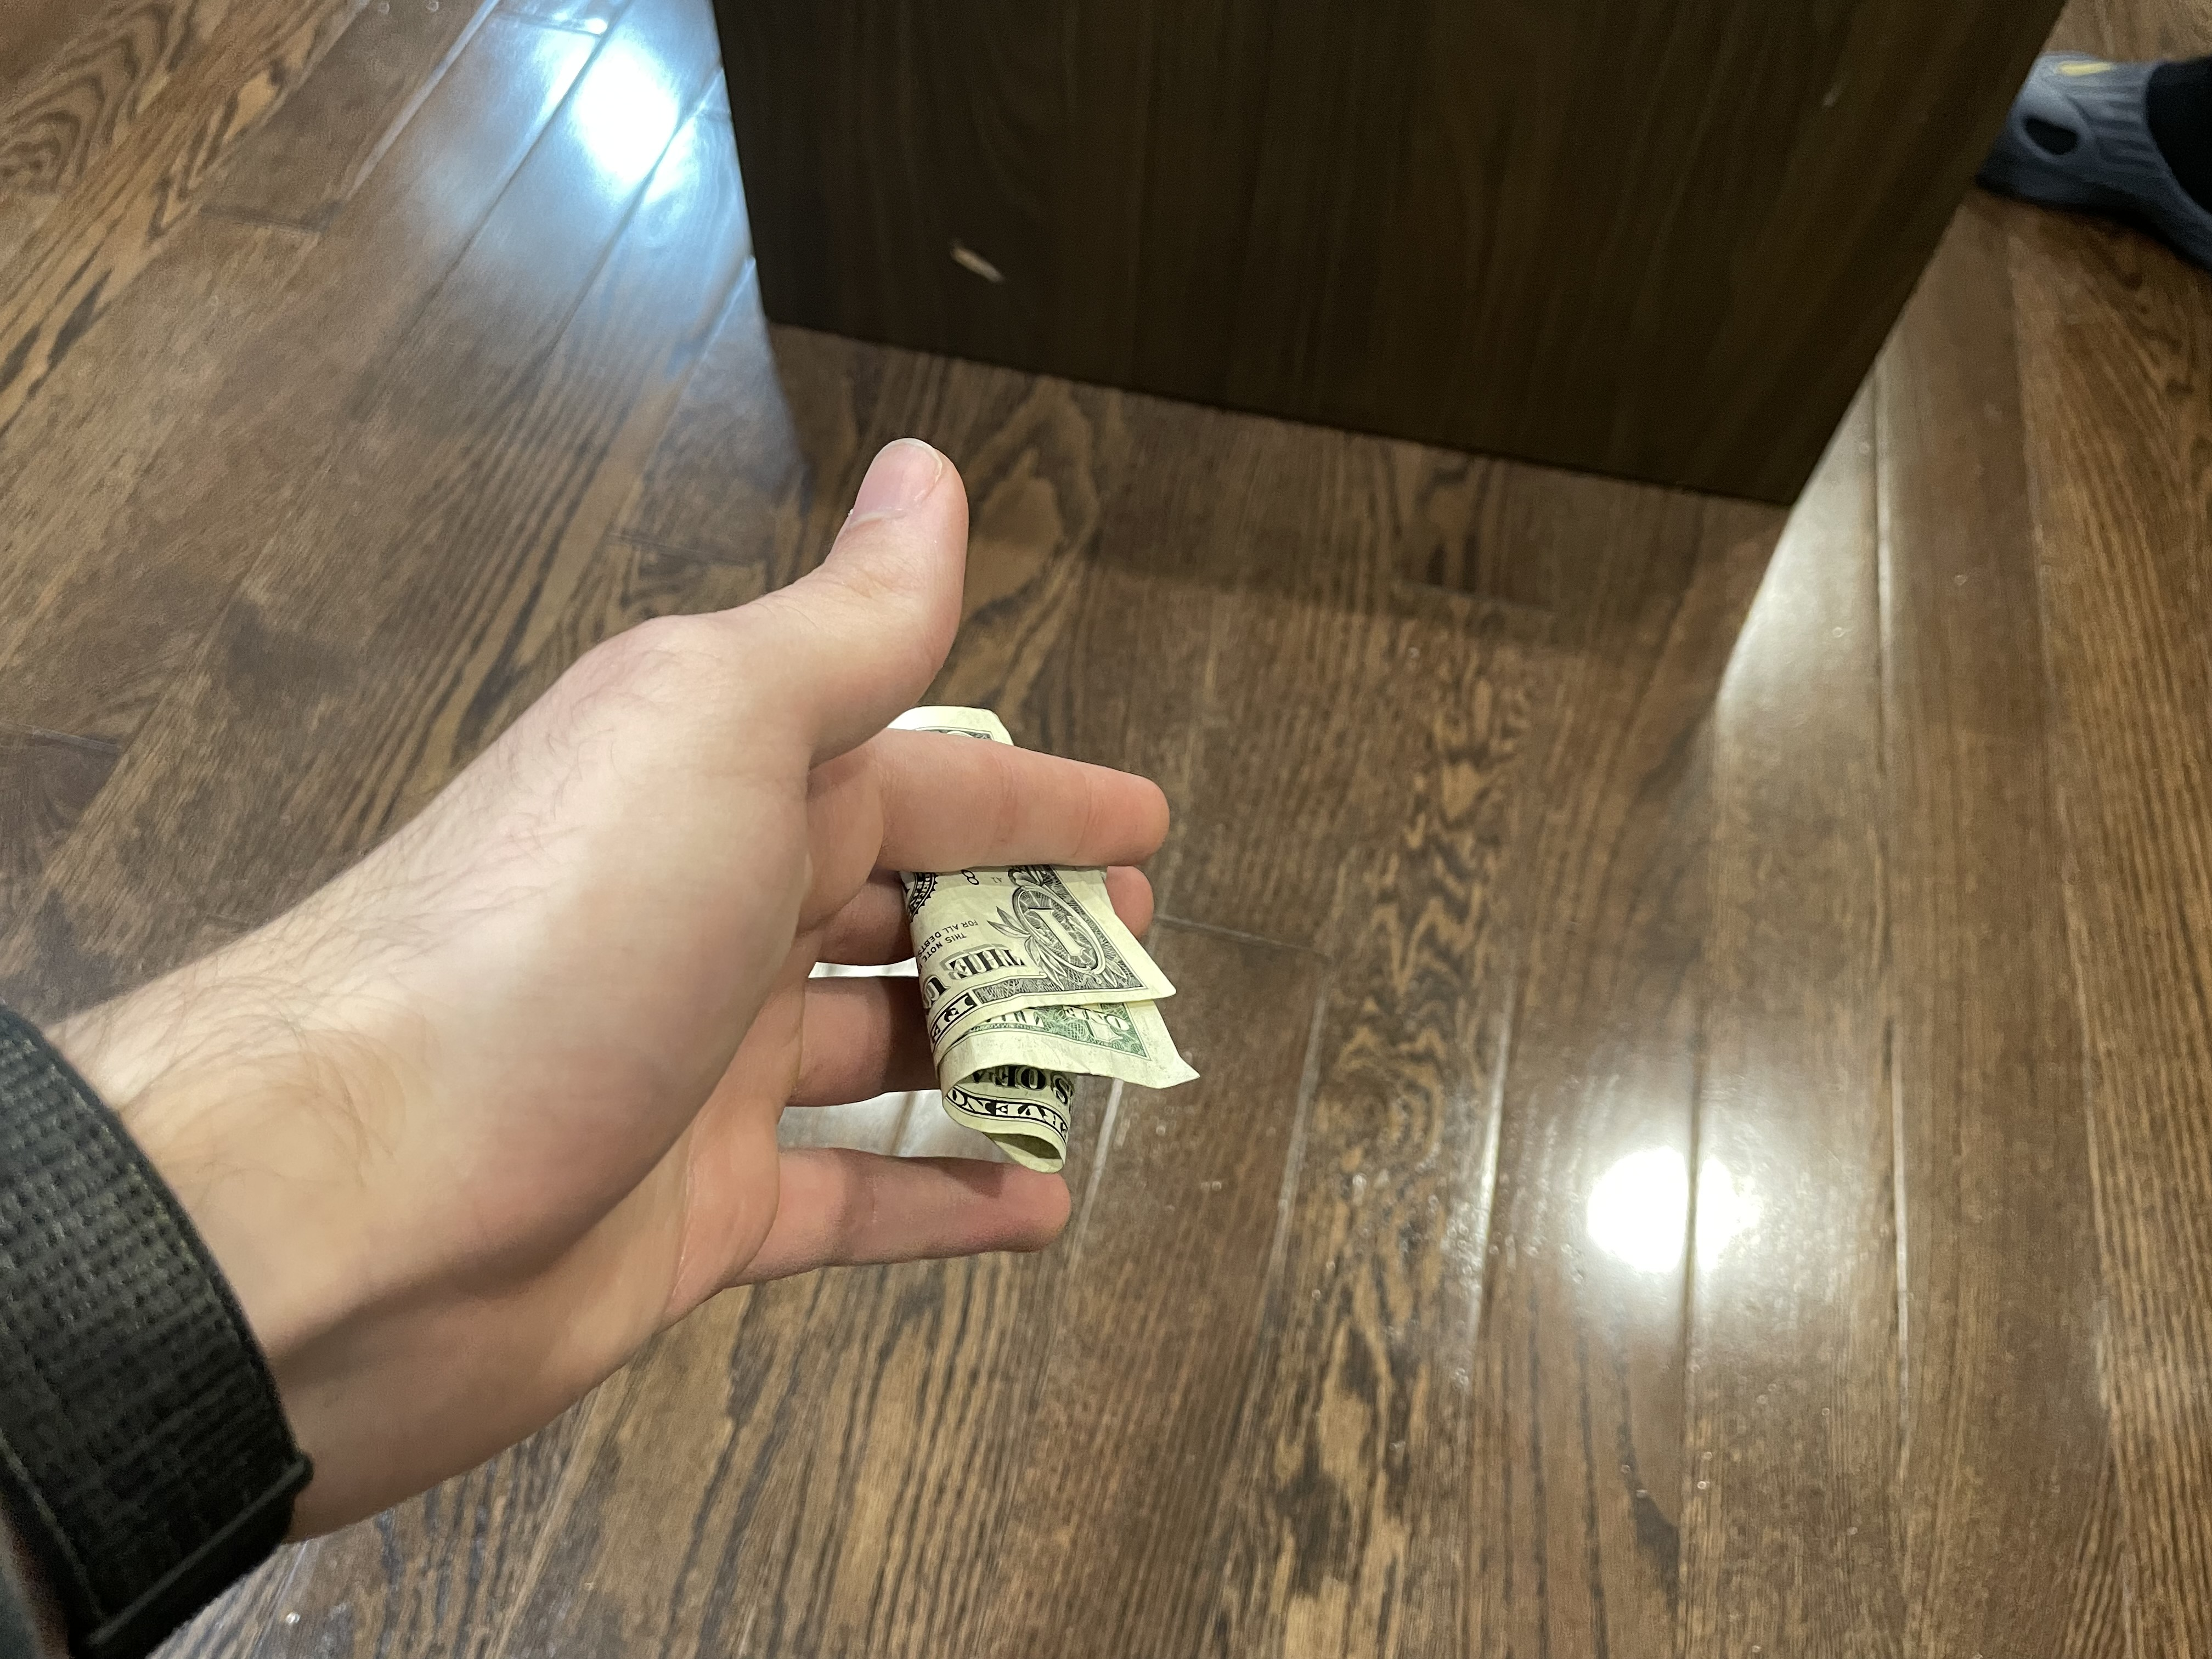
\includegraphics[scale=0.1]{img/cv/money/one_dollar_bill_hard.jpeg}
\caption{Difficult example of a one dollar bill.}
\label{fig:one_dollar_hard}
\end{figure}

To train on this dataset, it was first split into training and validation sets at a ratio of 75\% for training and 25\% for validation. The PyTorch deep learning library was then used to train a ResNet-50 CNN on this dataset. Back in the Fall 2021 term, a ResNet-34 was trained on the preliminary dataset, but we found that increasing the size of the model to ResNet-50 improved performance. Figure \ref{fig:resnet} has a diagram showing the architecture of the ResNet-18 model. Note that the ResNet-50 is simply a scaled up version of the ResNet-18, and the ResNet-18 architecture is just shown since it fits into a single diagram with no issues. Before feeding the images into the CNN, they were scaled down to a resolution of 384x384 to reduce inference time. Some data augmentation was also applied to increase the robustness of the trained classifier. The augmentations that were applied are:

\begin{enumerate}
    \item Rotate the bill by a random angle from -180 to 180 degrees. This was done to ensure the model is invariant to rotated bills.
    \item Crop the image in a random location with a random sized crop. This was done to ensure the model is invariant to the location and size of the bill in the image.
    \item Apply Gaussian blur with a random standard deviation. This was done to help the model be more robust to blurred images.
    \item Apply colour jitter with a random strength. This was done to help the model be more robust to changes in brightness, contrast, saturation, and hue.
\end{enumerate}

\begin{figure}[H]
\centering
\frame{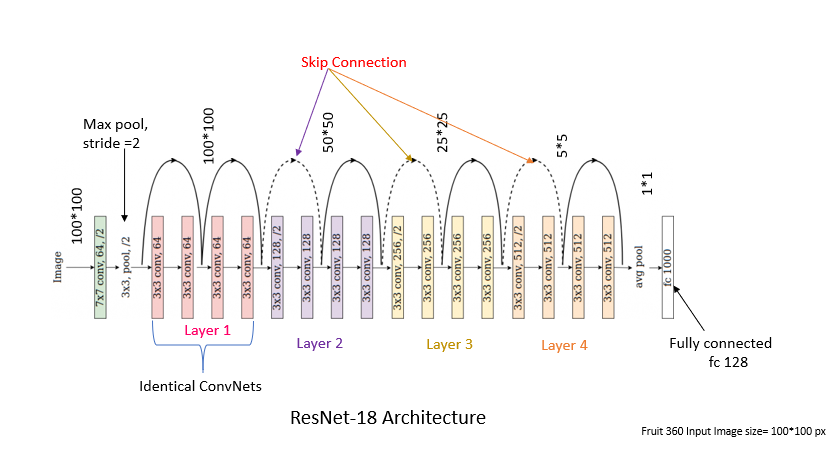
\includegraphics[scale=0.5]{img/cv/money/resnet18.png}}
\caption{Diagram displaying the ResNet-18 CNN architecture. \cite{resnet}}
\label{fig:resnet}
\end{figure}

The Weights \& Biases library was used to perform a hyperparameter sweep in order to find the hyperparameter values that give the best performance. The Weights \& Biases sweep library uses Bayesian optimization to iteratively choose hyperparameter values and evaluate their performance until the sweep is terminated. The hyperparameters that were tuned are the learning rate, weight decay, and number of frozen layers. In the end, the optimized model managed to achieve a validation accuracy of 97.1\%. The accuracy curves and validation confusion matrix can be seen in Figures \ref{fig:train_acc} to \ref{fig:conf_matrix}.

\begin{figure}[H]
\centering
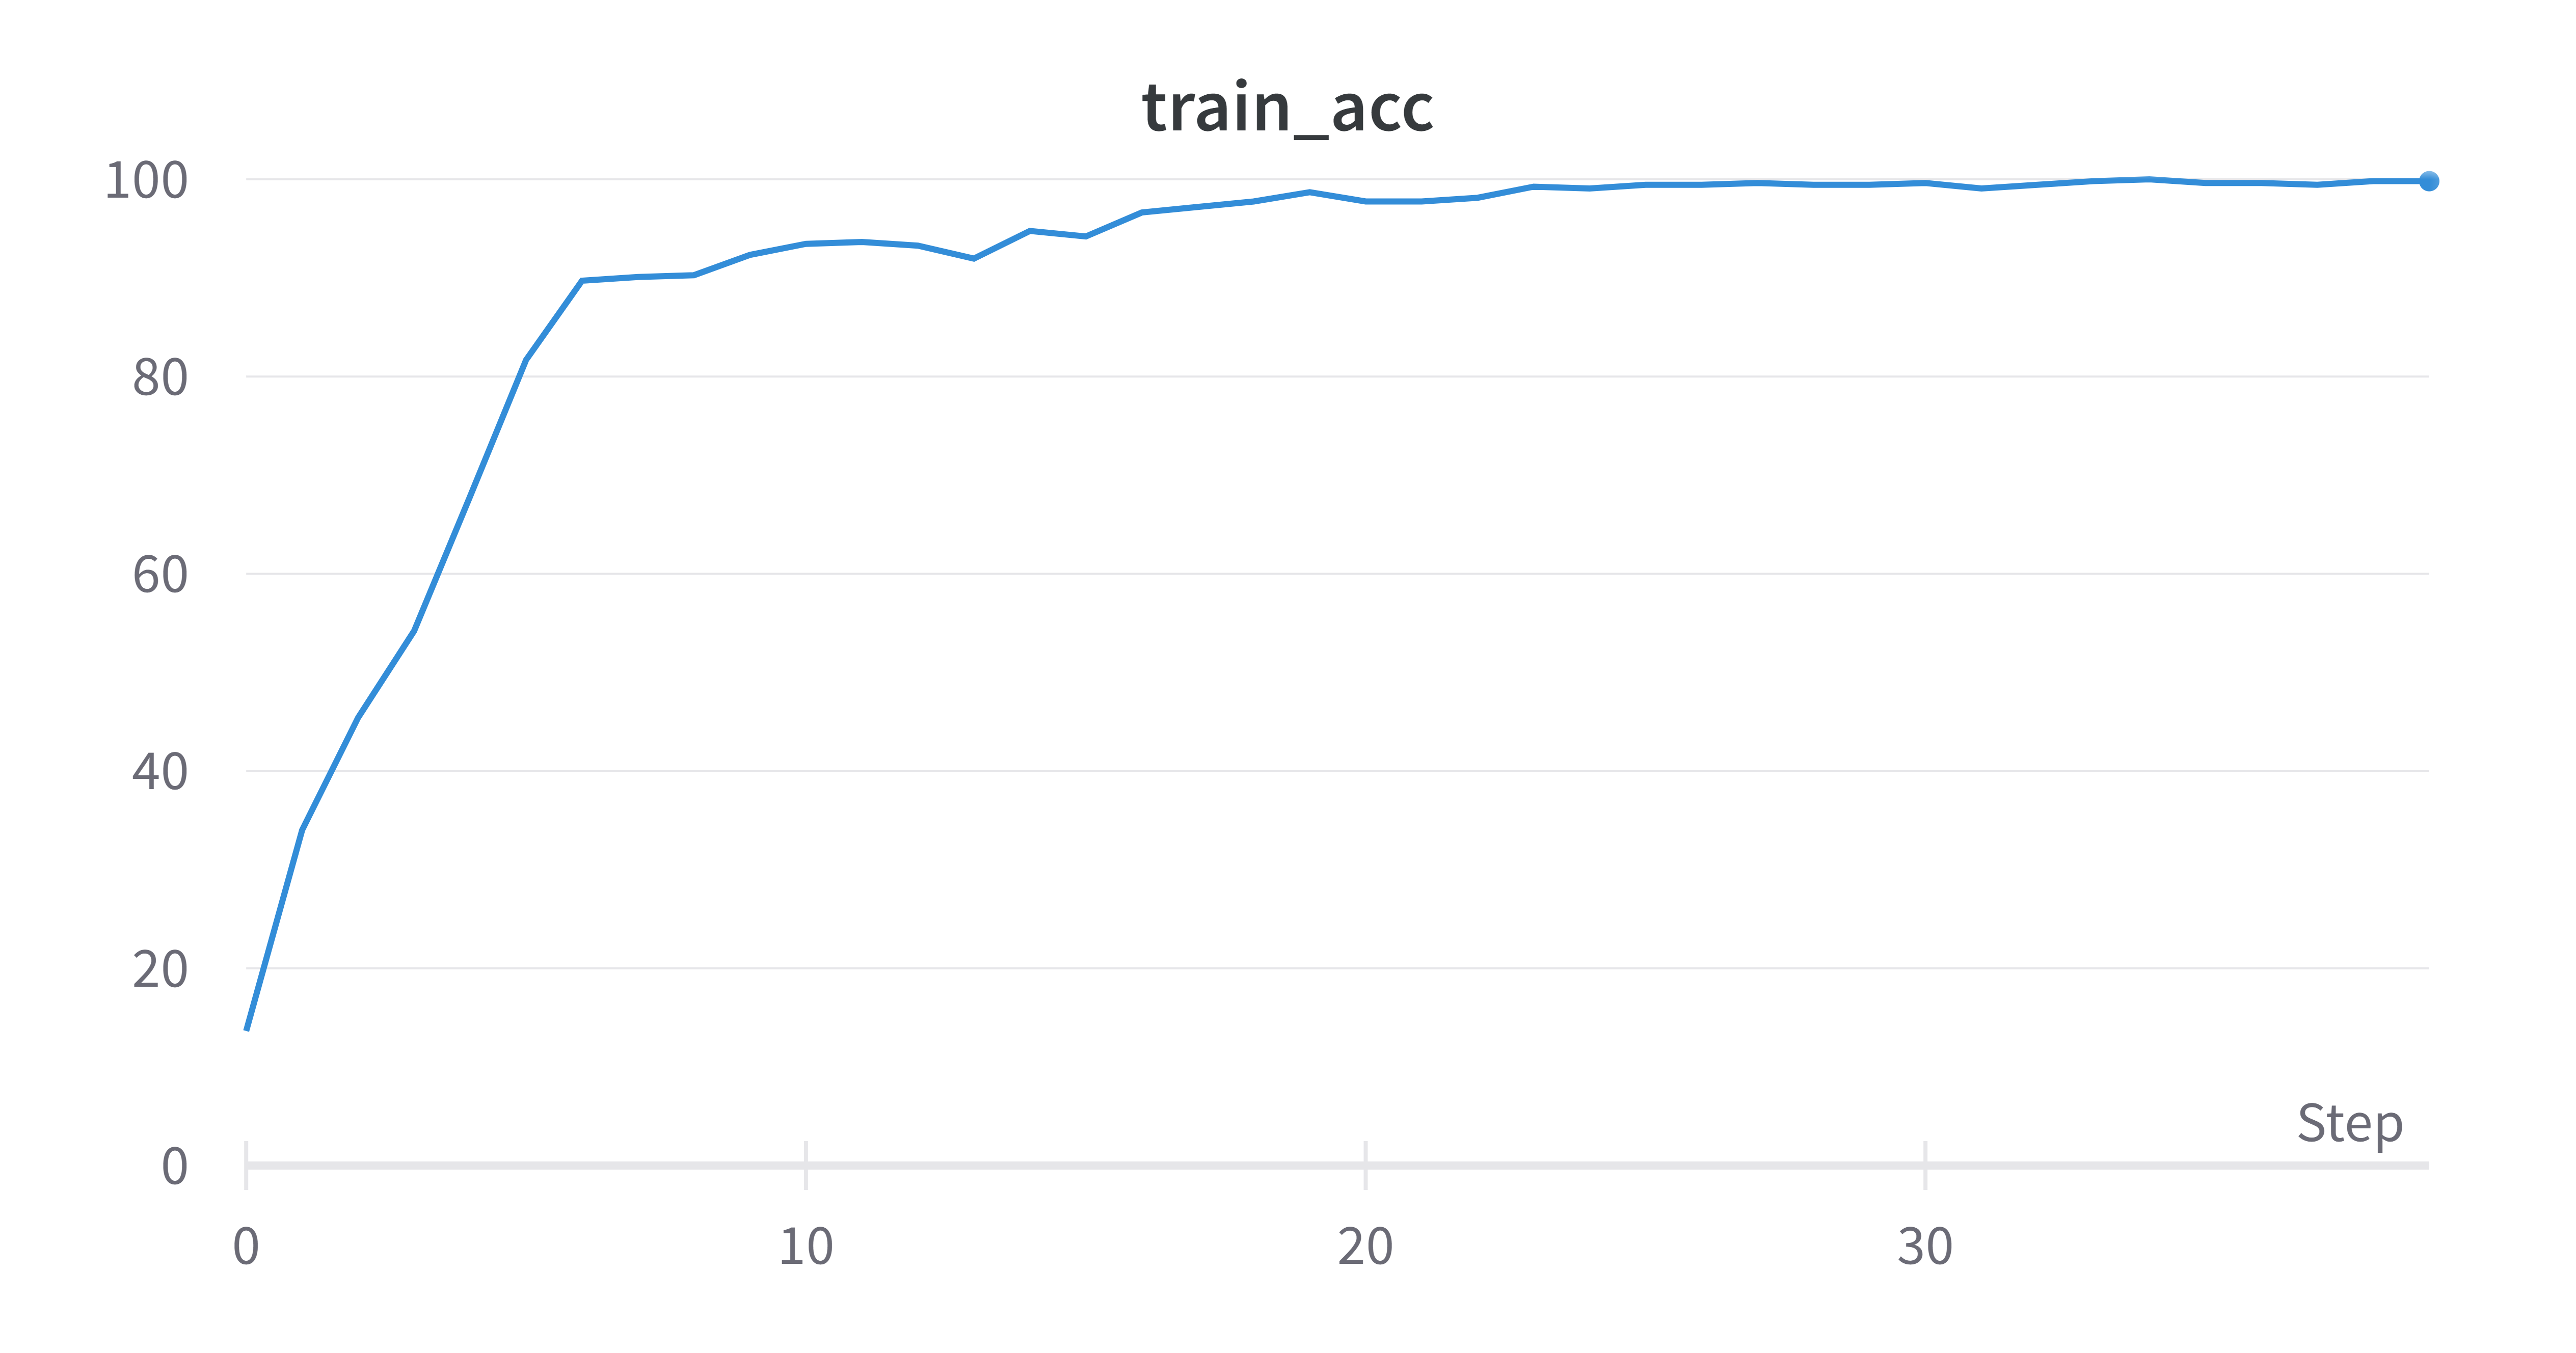
\includegraphics[scale=0.09]{img/cv/money/train_acc.png}
\caption{Plot of training accuracy per epoch for the best run.}
\label{fig:train_acc}
\end{figure}

\begin{figure}[H]
\centering
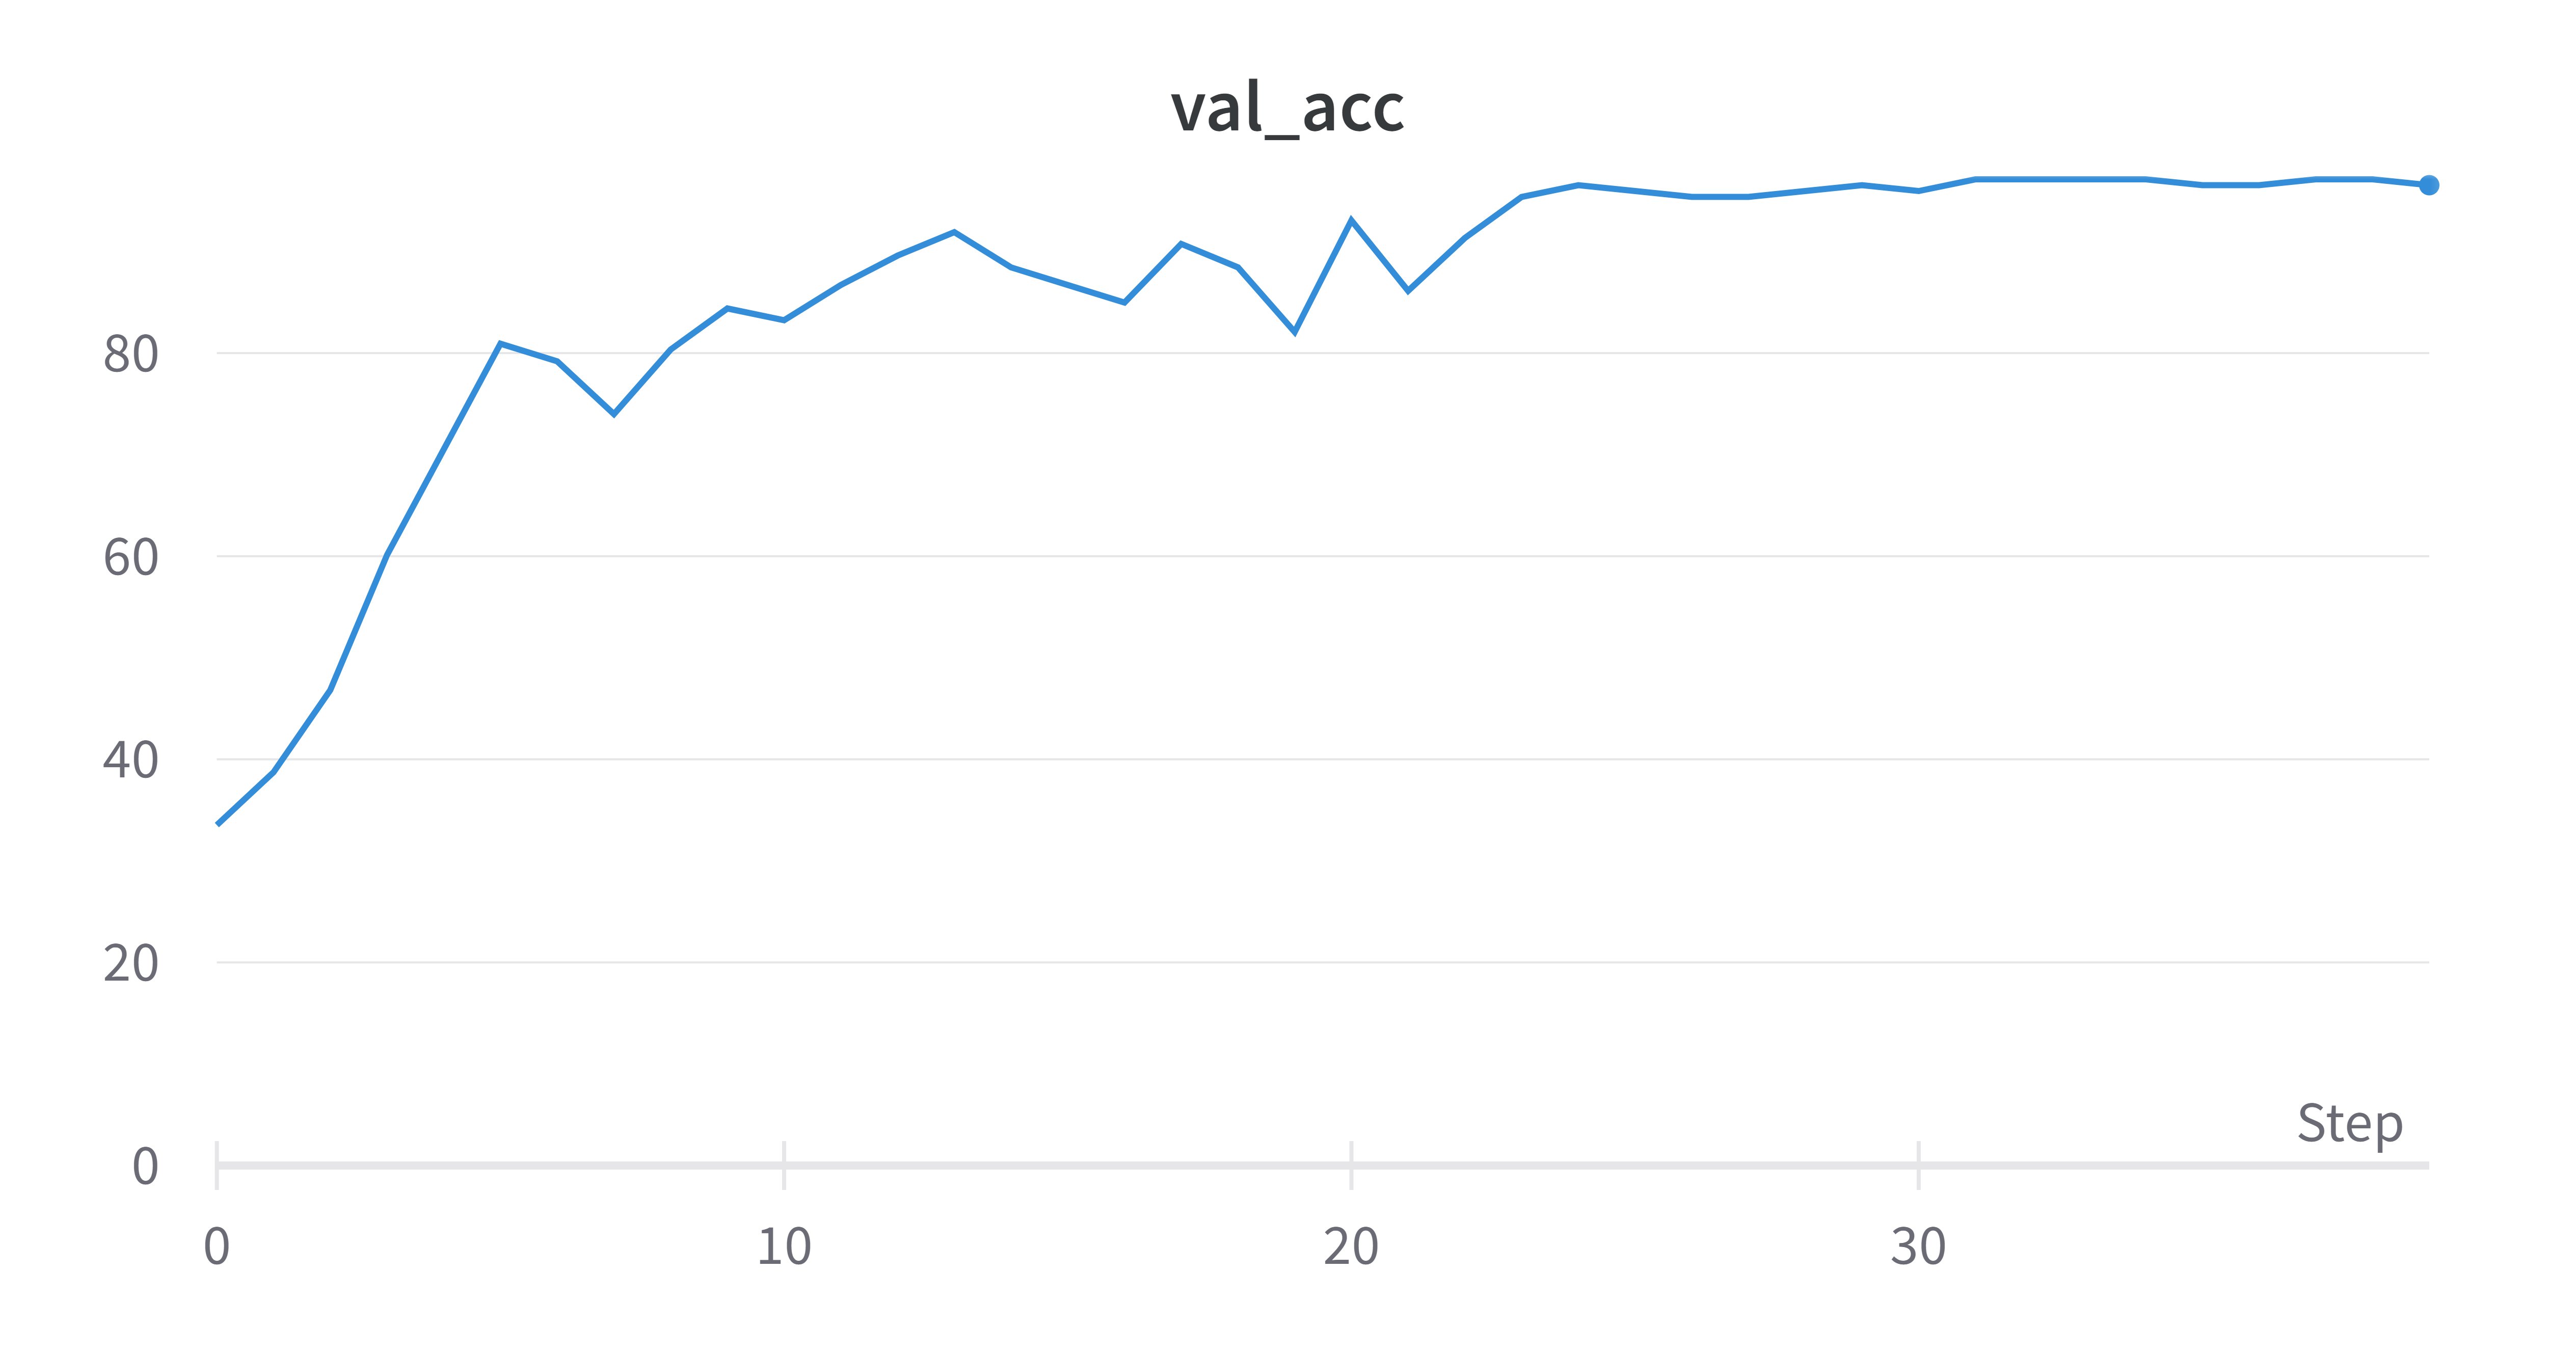
\includegraphics[scale=0.09]{img/cv/money/val_acc.png}
\caption{Plot of validation accuracy per epoch for the best run.}
\label{fig:val_acc}
\end{figure}

\begin{figure}[H]
\centering
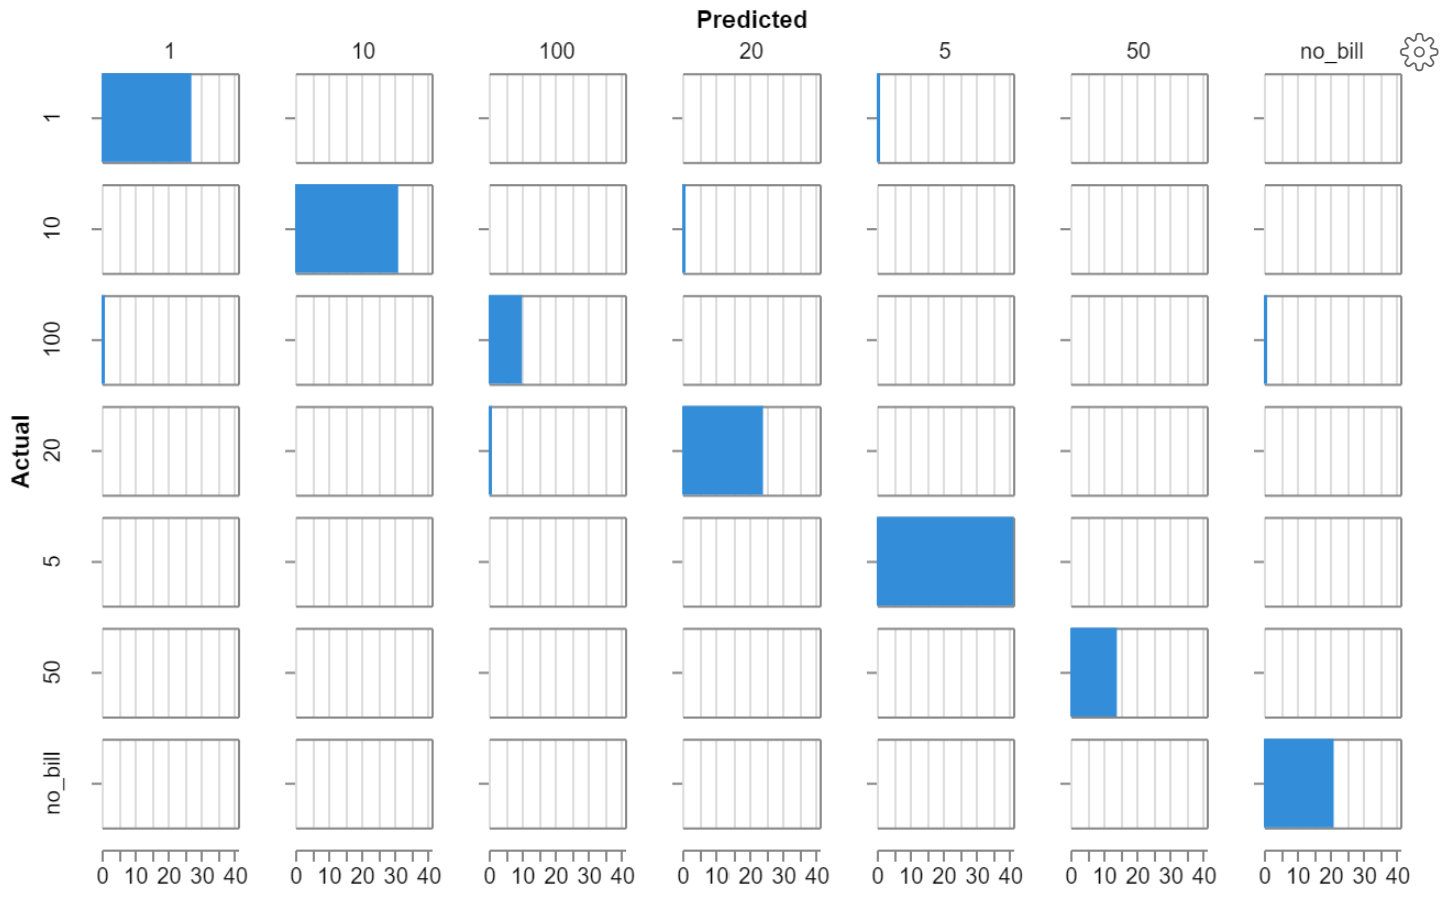
\includegraphics[scale=0.8]{img/cv/money/conf_matrix.png}
\caption{Confusion matrix on the validation set for the best run.}
\label{fig:conf_matrix}
\end{figure}

As can be seen in the confusion matrix, the classifier performs well on the given dataset and can robustly classify various bill images. If pursued further, the performance of the model could be improved greatly by simply increasing the size of the dataset.

\subsection{iOS App}
\subsubsection{UI/UX Design}
The final version of the iOS app uses similar design language to the initial prototypes, albeit with a different colour scheme. We found that while unique, the 'colourblind-safe' palette we had initially designed wasn't preferred by sighted users, and did not provide any substantial advantage over black and white. In fact, the coloured version had slightly worse text readability due to the lower contrast between the dark blue text and yellow background, as compared to black text on a white background.

\begin{figure}[H]
\centering
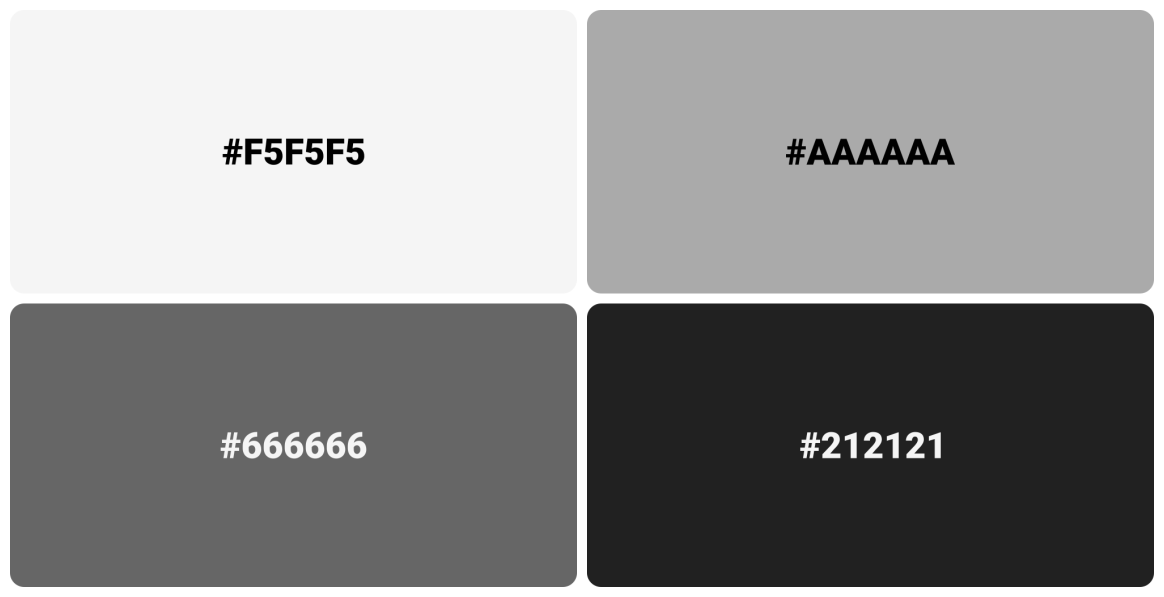
\includegraphics[scale=0.5]{img/app/mono_swatch.png}
\caption{Colour palette, with hex codes}
\label{fig:mono_swatch}
\end{figure}

We also updated the playback screen to function as a modal, rather than a standalone page. In terms of design language, the transience of the playback page is much better suited to a modal format, which can be easily dismissed and provides more minimal functionality. The home screen of the app is functionally unchanged; the same design principles of large text/buttons, high contrast, and minimalism are applicable to the new application as well as the old one, so the design was carried over and polished.

\begin{figure}[H]
\centering
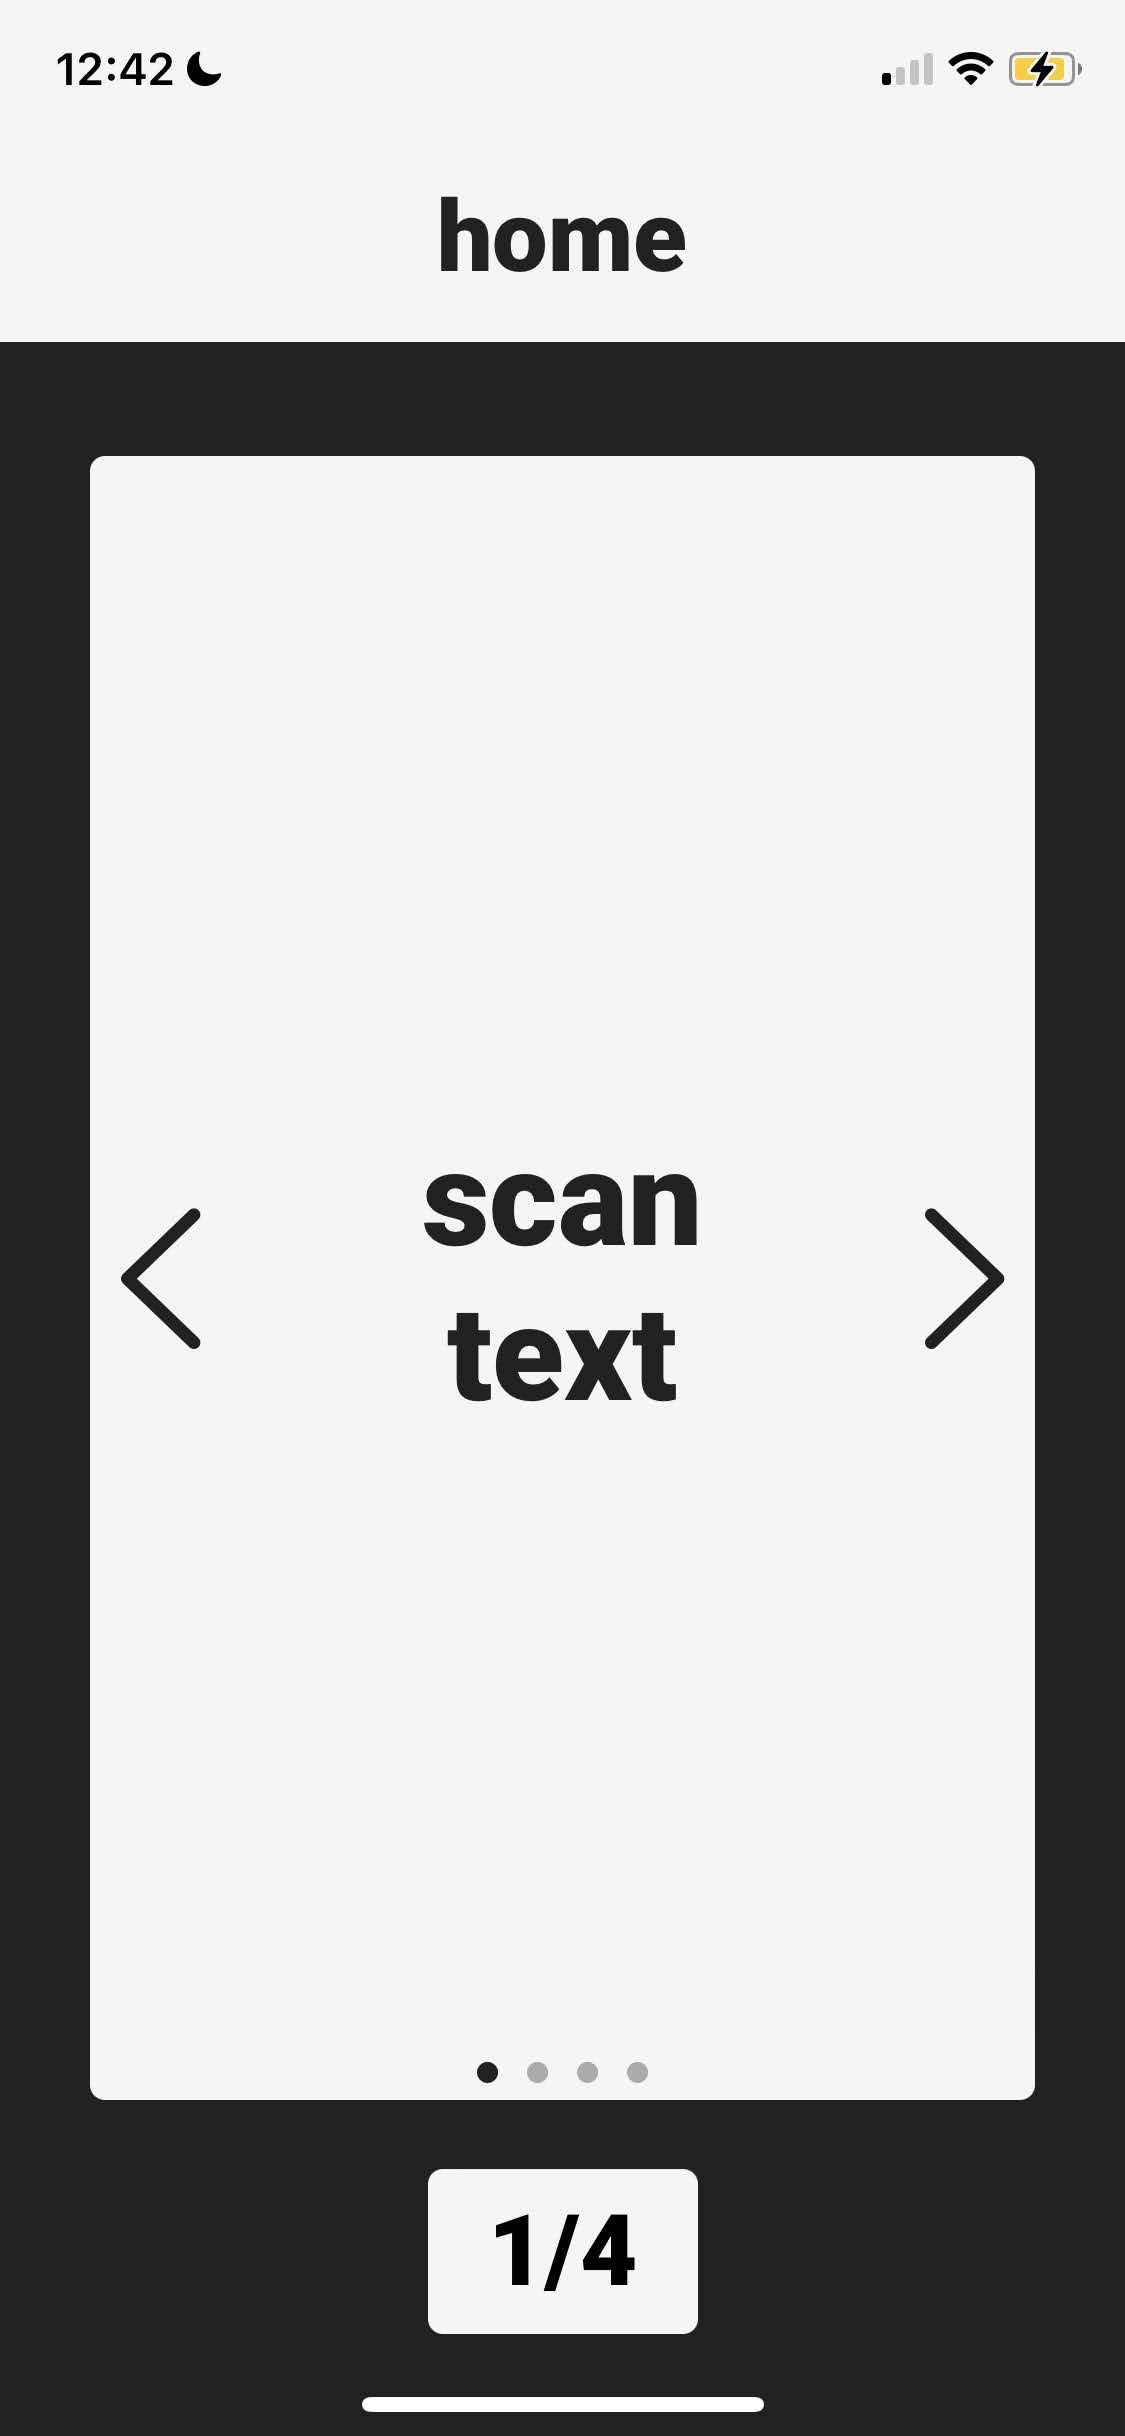
\includegraphics[scale=0.2]{img/app/landing.png}
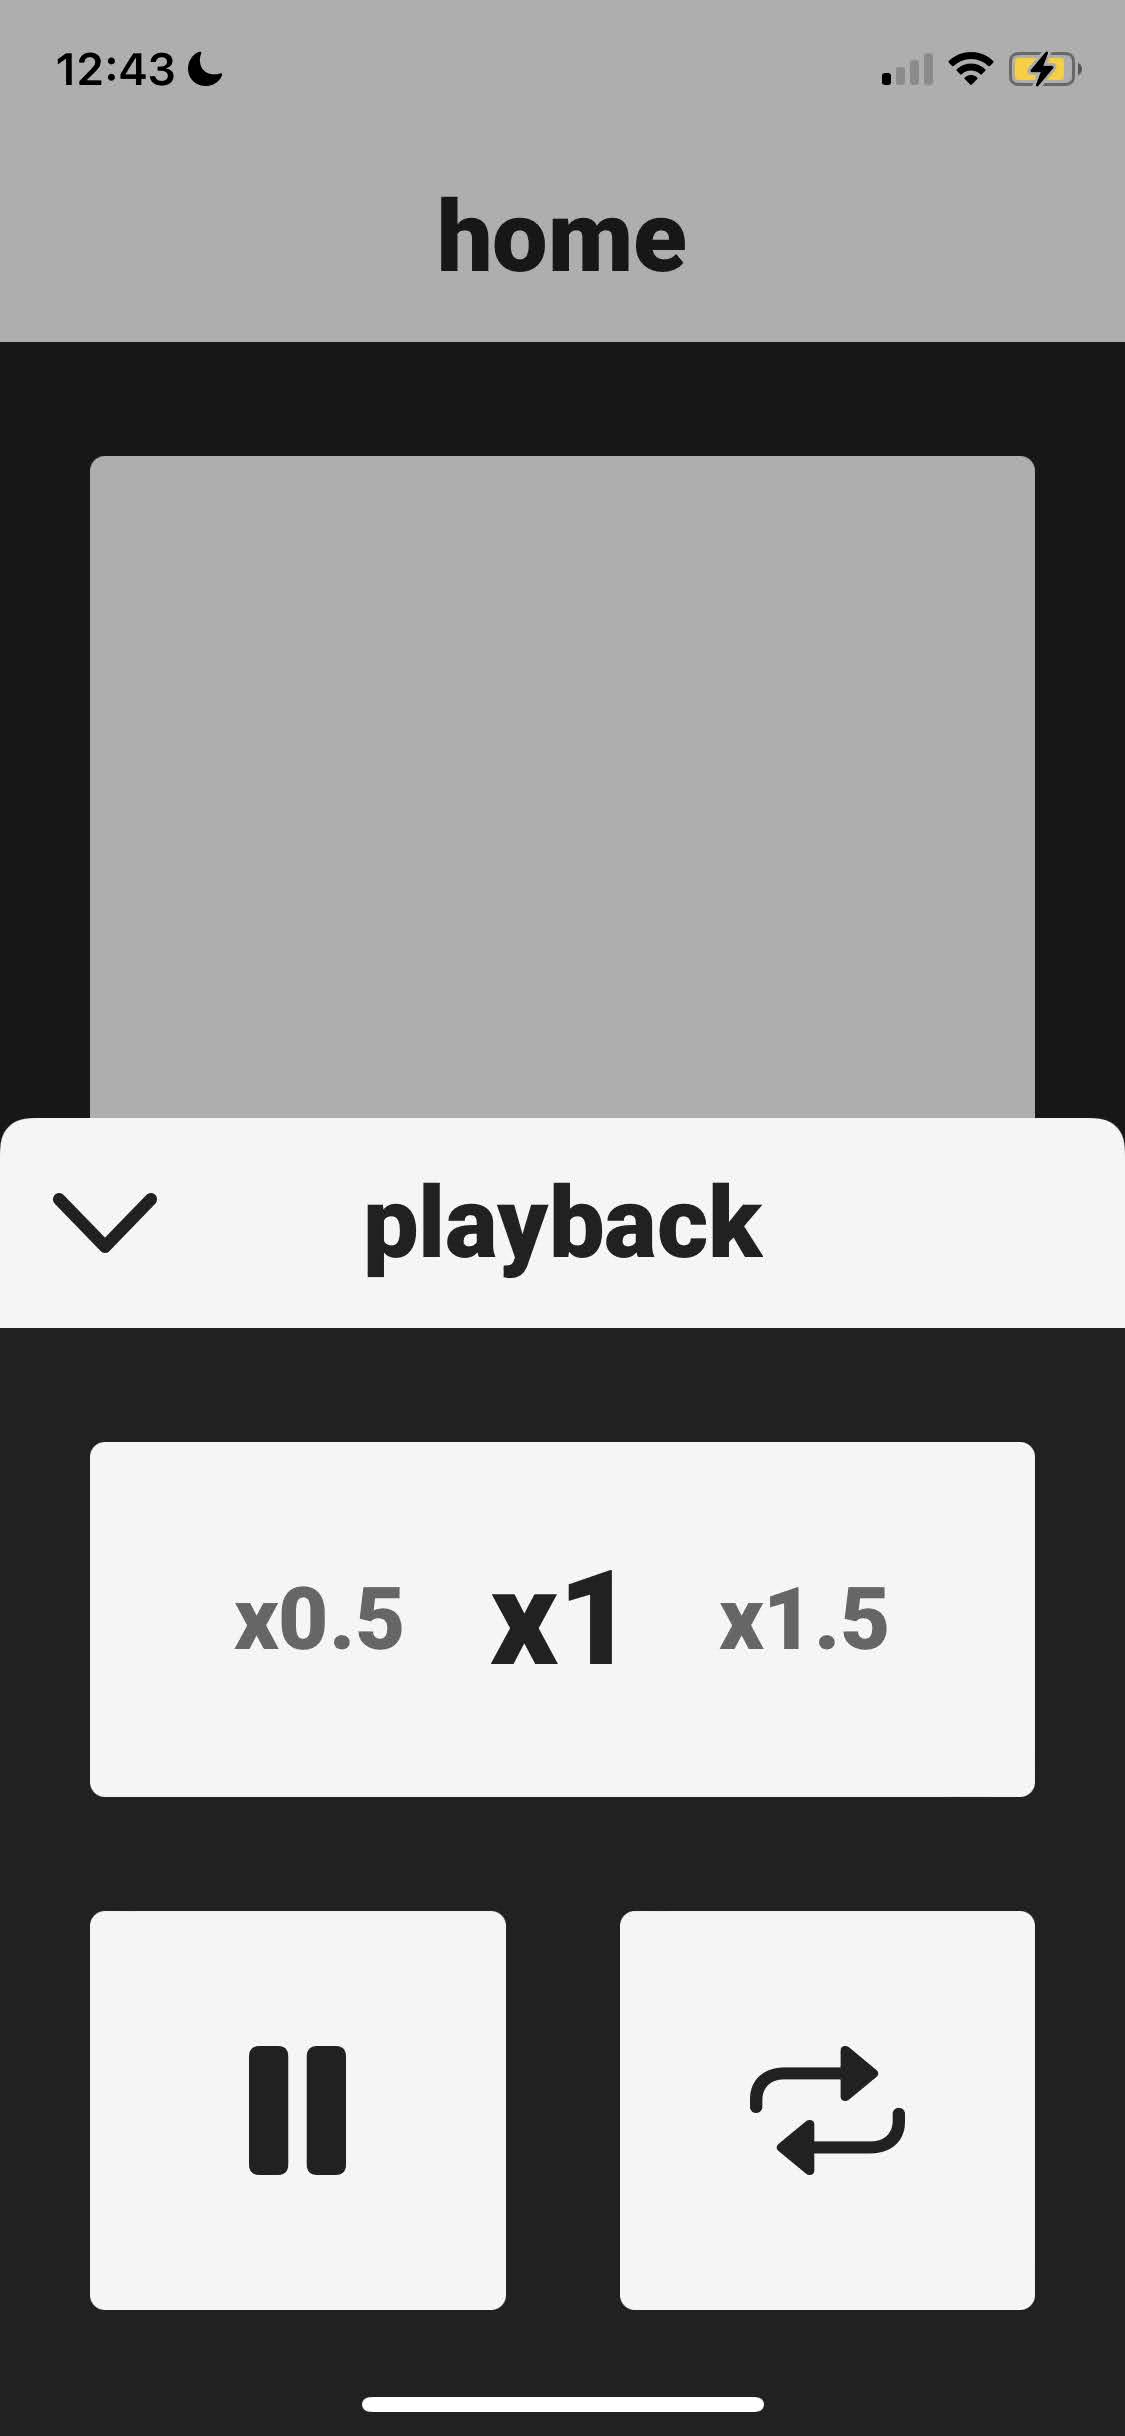
\includegraphics[scale=0.2]{img/app/playback.png}
\caption{App landing page/playback modal}
\label{fig:app_screenshots}
\end{figure}
\newpage

Finally, the app has full-featured VoiceOver support, using Apple's latest accessibility features. This means that although the main screen has a carousel of buttons, a user interacting with it using VoiceOver will 'see' it as a series of stacked buttons which they can iterate through as though it was a list. Some features targeted towards sighted users are ignored by VoiceOver, such as the arrow buttons used to navigate between buttons. The 'positioning' of some elements is also changed. In mobile design for sighted users, high priority elements are placed near the user's thumb, and low-priority ones are placed at the top of the screen so that they are out of the way. For VoiceOver users, this means that the least important elements will be read first, which is obviously undesirable. By leveraging some of the new iOS VoiceOver features, we were able to reorganize the order in which button labels etc are read out, such that the most important elements appear first.

\newpage
\begin{landscape}
    \subsection{Engineering Design Specification}
    \subsubsection{v0.1}
    \begin{center}
        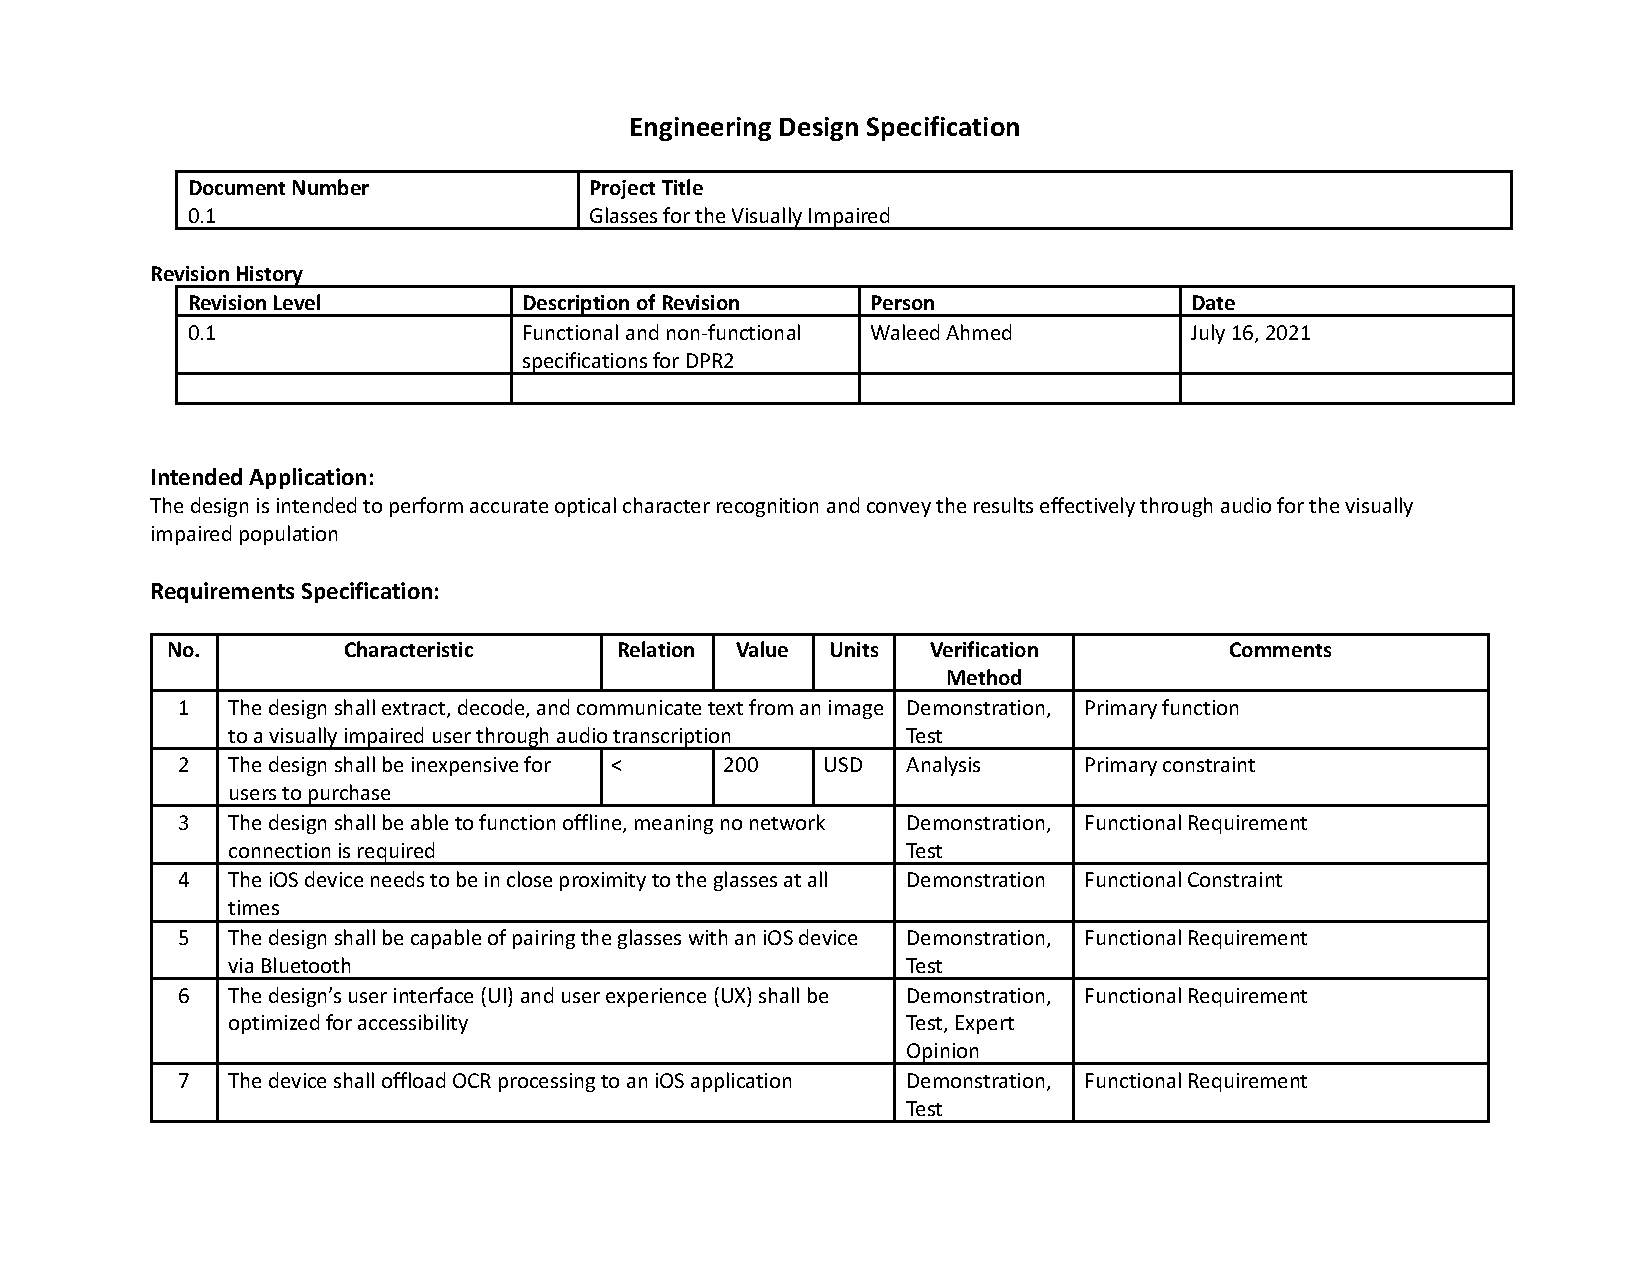
\includegraphics[page=1,width={0.86\linewidth}]{pdf/eds_0.1.pdf}
        \newpage
        \includegraphics[page=2,width={0.86\linewidth}]{pdf/eds_0.1.pdf}
    \end{center}
    
    \newpage
    \subsubsection{v0.2}
    \label{eds-0.2}
    \begin{center}
        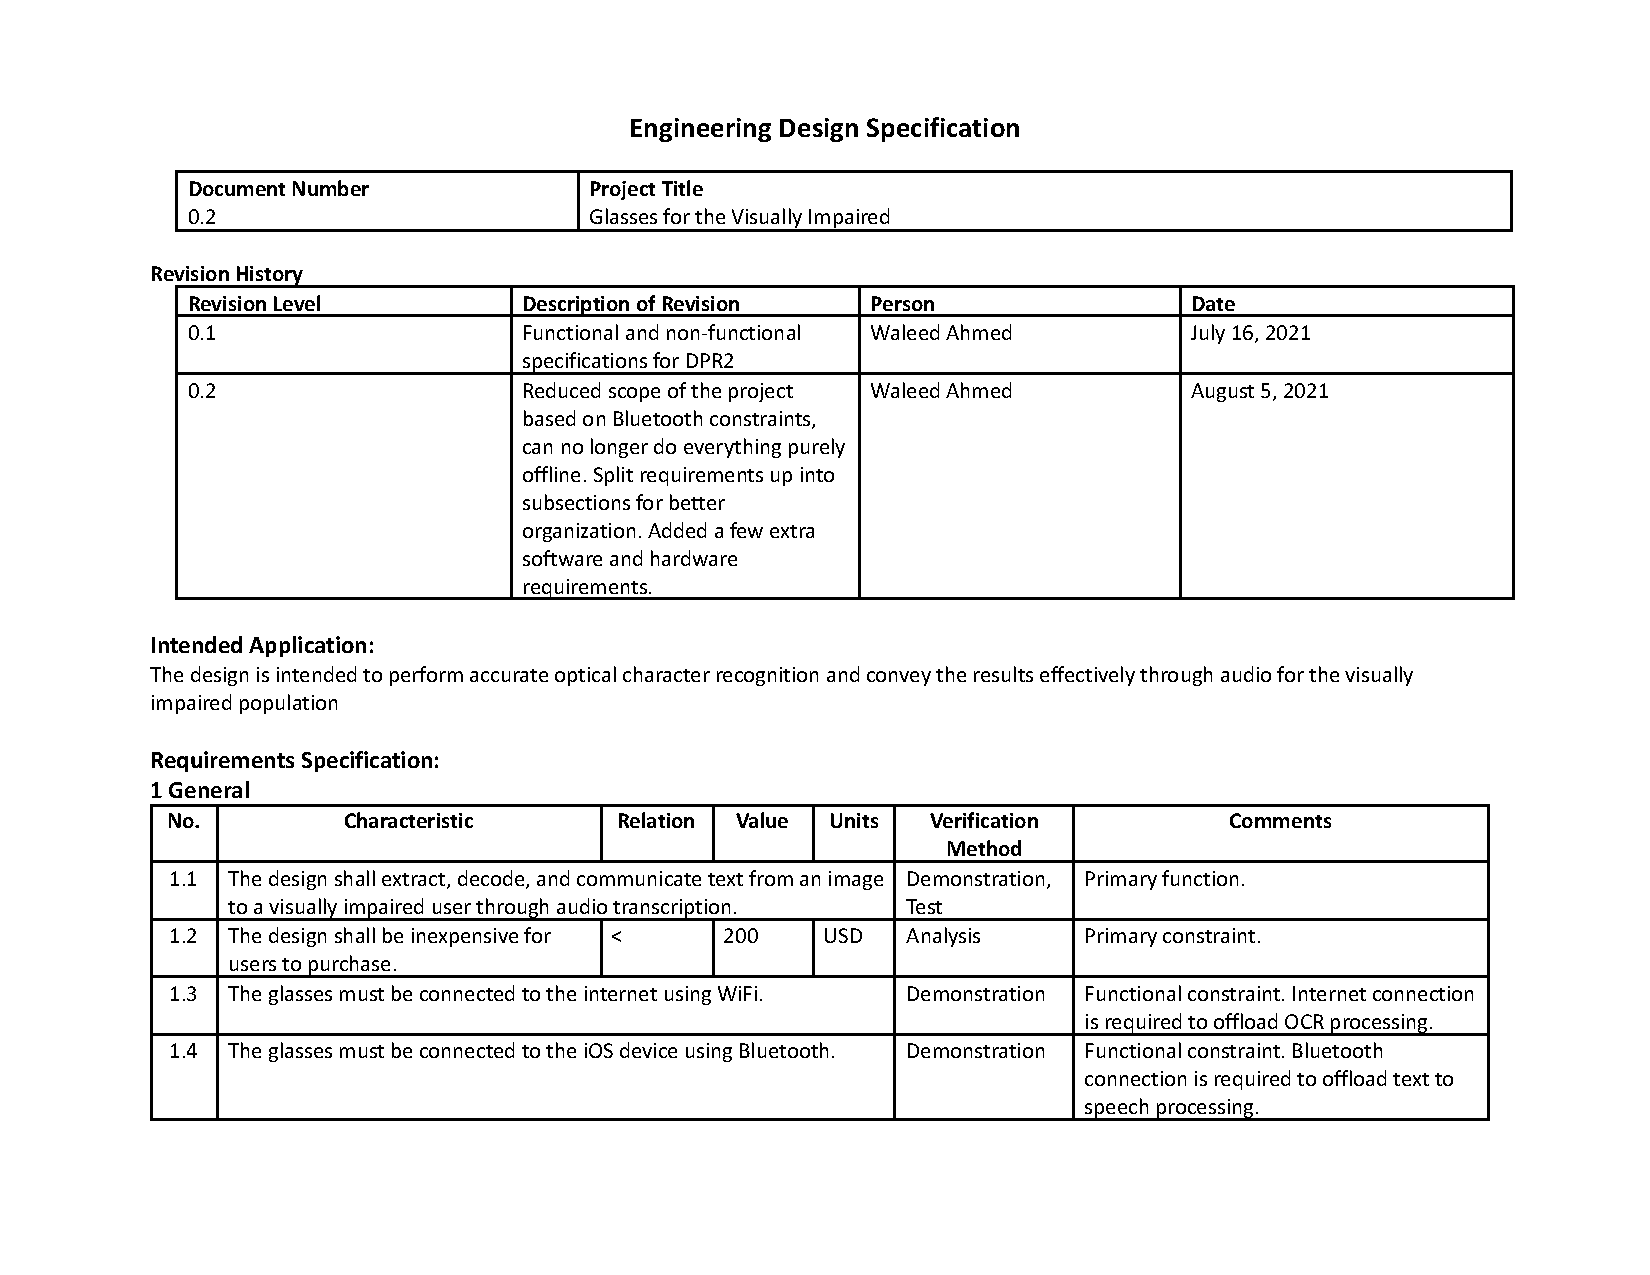
\includegraphics[page=1,width={0.86\linewidth}]{pdf/eds_0.2.pdf}
        \newpage
        \includegraphics[page=2,width={0.86\linewidth}]{pdf/eds_0.2.pdf}
        \newpage
        \includegraphics[page=3,width={0.86\linewidth}]{pdf/eds_0.2.pdf}
    \end{center}
    
    \newpage
    \subsubsection{v0.3}
    \label{eds-0.3}
    \begin{center}
        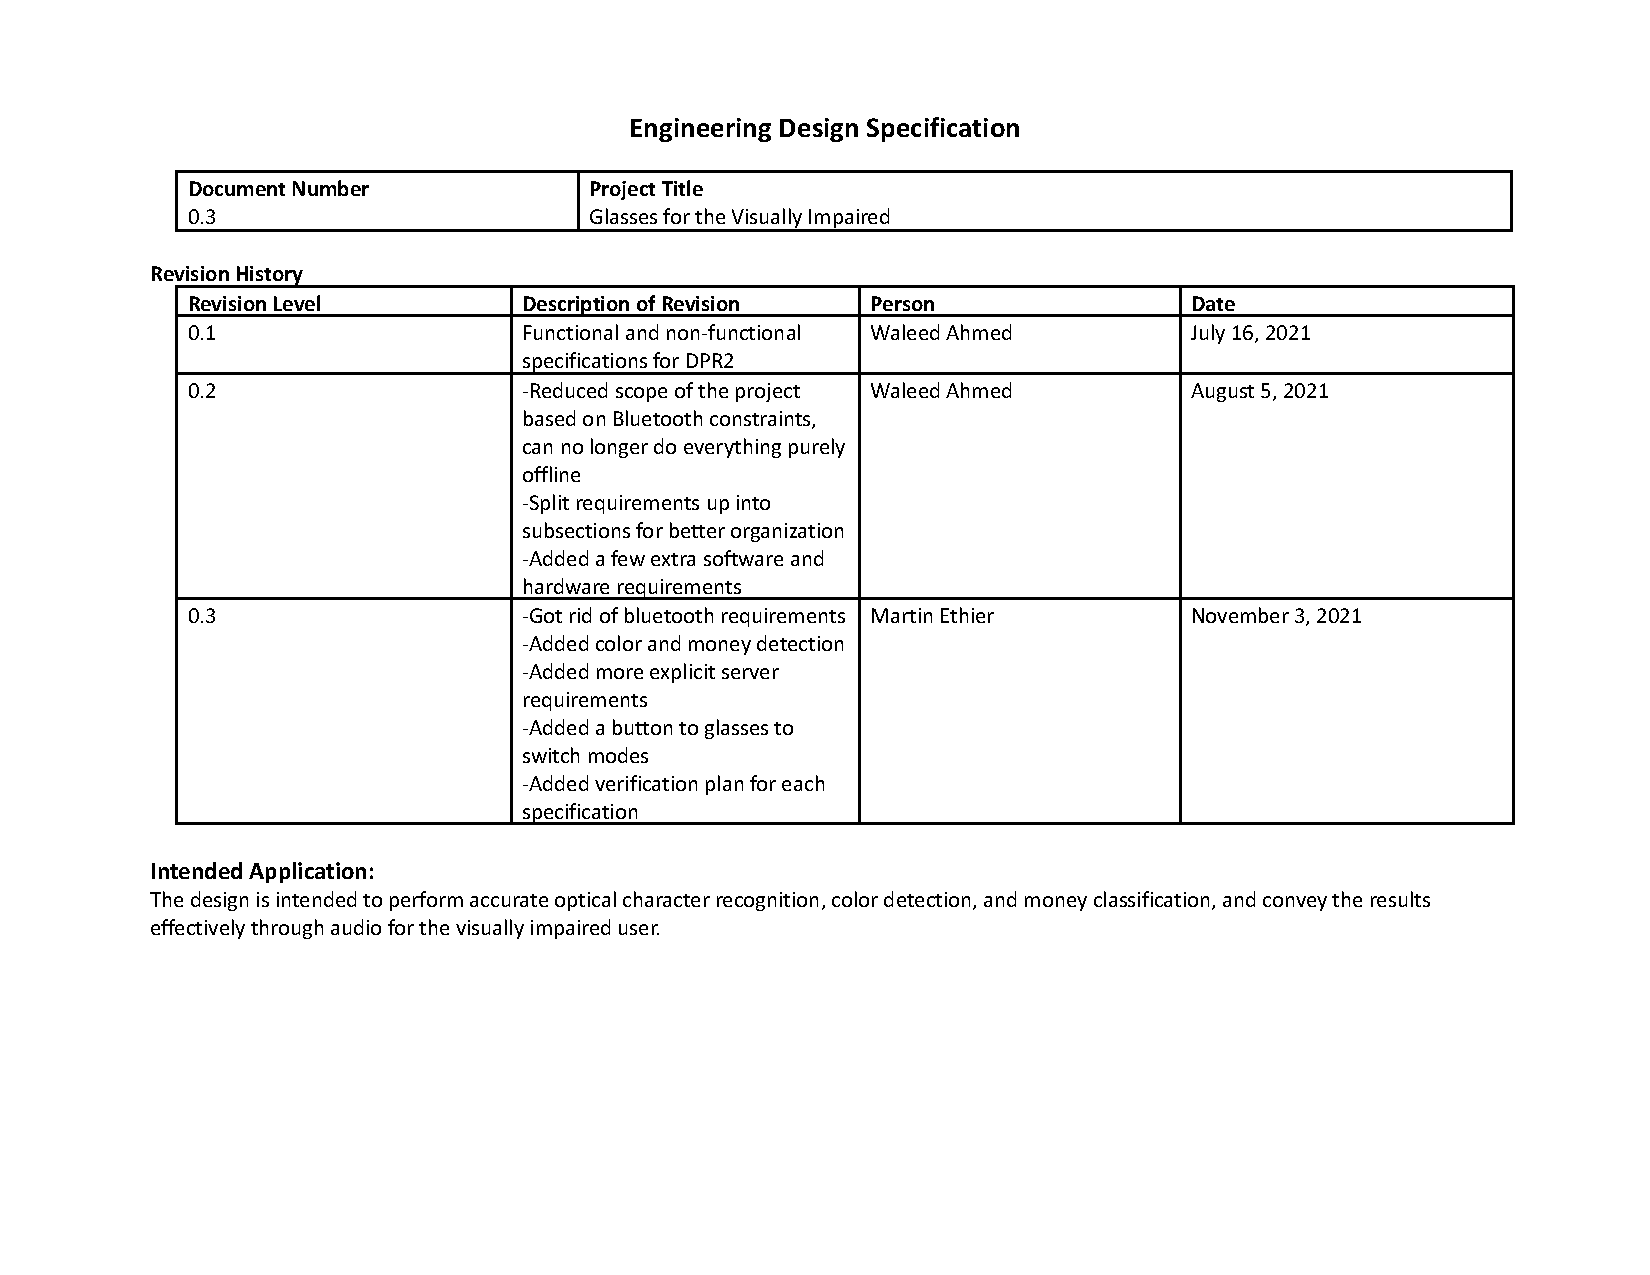
\includegraphics[page=1,width={0.86\linewidth}]{pdf/eds_0.3.pdf}
        \newpage
        \includegraphics[page=2,width={0.86\linewidth}]{pdf/eds_0.3.pdf}
        \newpage
        \includegraphics[page=3,width={0.86\linewidth}]{pdf/eds_0.3.pdf}
        \newpage
        \includegraphics[page=4,width={0.86\linewidth}]{pdf/eds_0.3.pdf}
        \newpage
        \includegraphics[page=5,width={0.86\linewidth}]{pdf/eds_0.3.pdf}
    \end{center}
    
        \newpage

    \subsubsection{v1.0}
    \label{eds-1.0}
    \begin{center}
        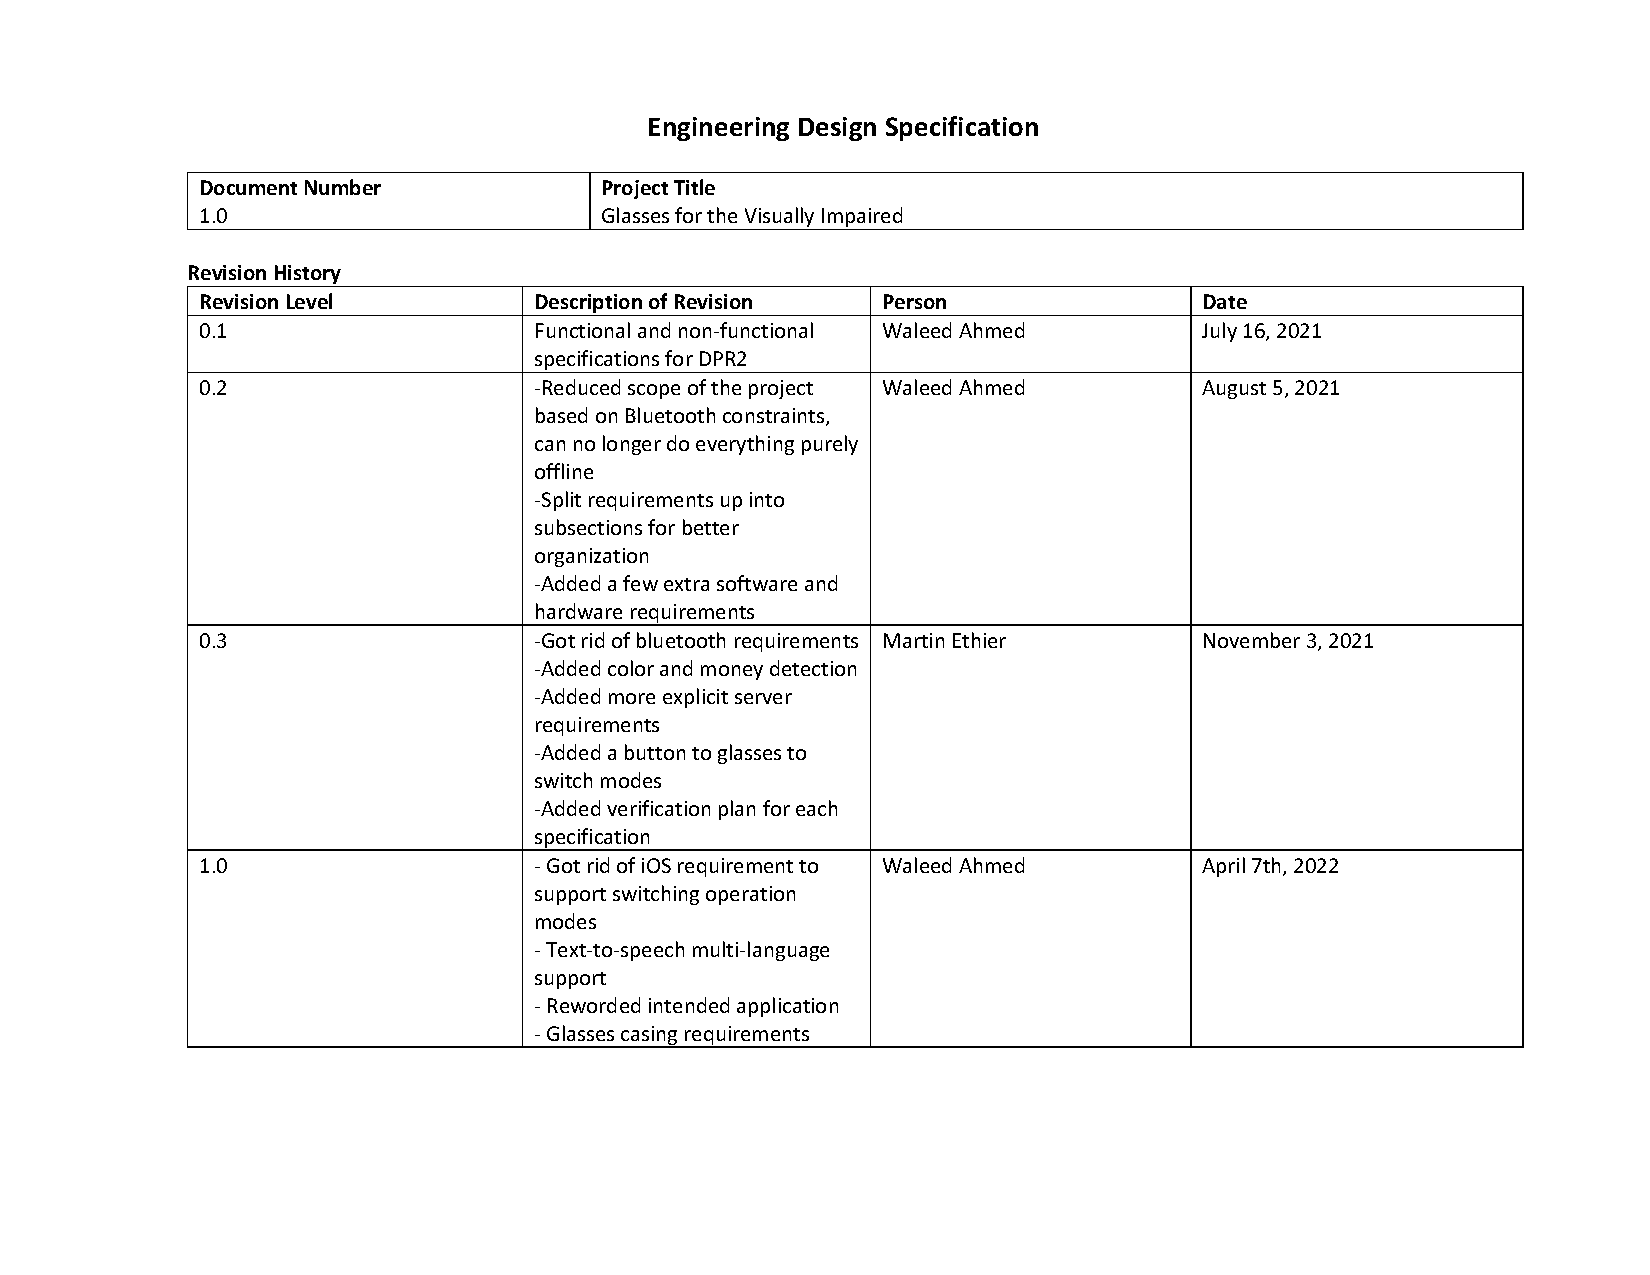
\includegraphics[page=1,width={0.86\linewidth}]{pdf/eds_1.0.pdf}
        \newpage
        \includegraphics[page=2,width={0.86\linewidth}]{pdf/eds_1.0.pdf}
        \newpage
        \includegraphics[page=3,width={0.86\linewidth}]{pdf/eds_1.0.pdf}
        \newpage
        \includegraphics[page=4,width={0.86\linewidth}]{pdf/eds_1.0.pdf}
        \newpage
        \includegraphics[page=5,width={0.86\linewidth}]{pdf/eds_1.0.pdf}
        \newpage
        \includegraphics[page=6,width={0.86\linewidth}]{pdf/eds_1.0.pdf}
    \end{center}
\end{landscape}


\newpage
\section{Appendix B - Verification and Validation Data}
\subsection{Bluetooth}
\label{bluetooth}
We had initially planned to use a Bluetooth Low Energy (BLE) connection to facilitate image transferring between the Raspberry Pi and the user's iOS device. We based this requirement around Apple's CoreBluetooth framework \cite{apple-bluetooth}, and their restrictions on the amount of background processing iOS applications can perform. iOS has extremely aggressive memory and power management systems, which put apps into a suspended state when not in the foreground (i.e. when not open on the user's screen). Apple allows applications to request permission to perform background tasks, with certain limitations. One such permission is the ability to monitor communications from a paired BLE peripheral and act upon incoming data \cite{apple-bluetooth}. Once an incoming BLE packet destined for an application is detected, iOS provides a 15-30 second window for said application to complete any tasks it needs to do to react to this data before putting them back into a suspended state automatically.

We had planned to compress an image into JPEG format on the Raspberry Pi, then send a BLE notification to the iOS device that a new image was available for processing. The iOS device would then wake up the background application and pass along the BLE packet. The iPhone could then connect to the Raspberry Pi and retrieve the image. However, we discovered that BLE's extremely lightweight nature makes it impractical for transmitting large files (such as an image). The Raspberry Pi uses a Bluetooth 4.1 chip \cite{raspi-hardware}, which imposes a limit on the size of the data field in a transmitted BLE packet. The iPhone has a Bluetooth 4.2 chip \cite{iphone-hardware} which is capable of communicating with the Raspberry Pi's older chip, but is rate limited by the Pi's hardware. The maximum size of a data field in a packet sent between the two devices is therefore 27 bytes, although 4 of these bytes are used to store an offset (so that files larger than 27 bytes can be sent using consecutive packets. Additionally, iOS allows a maximum of 4 packets to be exchanged before a new BLE connection needs to be made. The BLE protocol also mandates a connection interval, which varies by device but is set to 15ms on all devices running iOS 11 or later \cite{apple-bluetooth}. This means that it would take almost a minute to transmit the smallest photo we could reasonably perform OCR on. This falls outside the window that iOS provides for a device to perform processing, before the application even receives the image.

Our workaround for this Bluetooth limitation was to drop the offline requirement and introduce a server between the glasses and iOS app that would be responsible for all the image processing and computer vision. See section \ref{server} for a detailed overview of the server.

A next step to bring our design closer to a final product would be to take advantage of the Apple MFi program \cite{apple-mfi}. This would allow us to remove the need for the server and honour our original requirement of having the glasses and iOS app work without a network connection. See section \ref{apple-mfi} for more.

\subsection{Apple MFi}
\label{apple-mfi}
Bluetooth Classic is a different version of Bluetooth which supports much higher throughput; BT Classic connections are two-way, continuous data streams up to 2.1Mbps \cite{bluetooth-classic}. iOS supports this version of Bluetooth, although it is restricted to embedded chips with Apple's MFi (Made For iPod) certification \cite{apple-mfi}. Using Bluetooth Classic would provide the data transfer speeds needed to send an image quickly enough to provide a good user experience, although the ability to perform background processing is restricted to BLE devices. Nevertheless, this would enable us to perform OCR on a piece of text and read it back while the user is offline. In our final product, we would apply for an Apple MFi certification in order to unlock the full potential of Bluetooth on iPhone.

\newpage
\section{Appendix C - Design Project Management Data}


\section{Appendix D - Knowledge Application}

\section{Exhibits}
\subsection{Promotional Video}
\subsection{Symposium Poster}
\subsection{GitHub}


\newpage
% REFERENCES
\begin{thebibliography}{9}
\bibitem{orbis-global-blind-data}
“Number of blind people set to triple by 2050” Orbis, 09-Feb-2021. [Online]. Available: https://can.orbis.org/en/news/2017/number-of-blind-people-set-to-triple-by-2050-1. [Accessed: 02-Aug-2021]. 

\bibitem{cnib-blind-data}
“Blindness in Canada” CNIB. [Online]. Available: https://cnib.ca/en/sight-loss-info/blindness/blindness-canada?region=on. [Accessed: 02-Aug-2021]. 

\bibitem{nfb-blind-data}
“Blindness Statistics” NFB, Jan-2019. [Online]. Available: https://nfb.org/resources/blindness-statistics. [Accessed: 02-Aug-2021]. 

\bibitem{lighthouse-sf-info-page}
“What does ‘blind’ really mean?” LightHouse for the Blind and Visually Impaired, 28-Jan-2019. [Online]. Available: https://lighthouse-sf.org/about/getting-started/. [Accessed: 02-Aug-2021]. 

\bibitem{WHO-blindness}
“Vision impairment and blindness” World Health Organization. [Online]. Available: https://www.who.int/news-room/fact-sheets/detail/blindness-and-visual-impairment. [Accessed: 02-Aug-2021]. 

\bibitem{lighthouse-sf-homepage}
LightHouse for the Blind and Visually Impaired, 22-Aug-2019. [Online]. Available: https://lighthouse-sf.org/. [Accessed: 02-Aug-2021].

\bibitem{uw-accessability}
AccessAbility Services, 08-Jul-2021. [Online]. Available: https://uwaterloo.ca/accessability-services/. [Accessed: 03-Aug-2021]. 

\bibitem{jaws-software}
“Jaws®” Freedom Scientific. [Online]. Available: https://www.freedomscientific.com/products/
software/jaws/. [Accessed: 03-Aug-2021].

\bibitem{kurzweil}
K. Education, Assistive learning technologies \& literacy software from KURZWEIL Education. [Online]. Available: https://www.kurzweiledu.com/default.html. [Accessed: 03-Aug-2021]. 

\bibitem{read-and-write}
“Read \& write for education - reading, literacy \& assistive software” Texthelp. [Online]. Available: https://www.texthelp.com/en-gb/products/read-and-write-education/. [Accessed: 03-Aug-2021]. 

\bibitem{speechify}
Speechify. [Online]. Available: https://speechify.com/. [Accessed: 03-Aug-2021]. 

\bibitem{clickup}
“ClickUp™ | one app to replace them all.” [Online]. Available: https://clickup.com/. [Accessed: 07-Aug-2021]. 

\bibitem{orcam}
OrCam MyEye 2.0. [Online]. Available: https://www.orcam.com/en/myeye2/. [Accessed: 08-Aug-2021].

\bibitem{orcam-price}
B. Holton, “MyReader and MyEye from OrCam: Text and item recognition at the touch of a finger,” The American Foundation for the Blind. [Online]. Available: https://www.afb.org/aw/18/2/15244. [Accessed: 08-Aug-2021]. 

\bibitem{orcam-amazon}
“OrCam MyEye Pro ,” Amazon.ca: Electronics. [Online]. Available: https://www.amazon.ca/OrCam-Inc-MyEye-2/dp/B07H31SBMW. [Accessed: 08-Aug-2021].

\bibitem{WHO-assistive}
“Assistive technology,” World Health Organization. [Online]. Available: https://www.who.int/news-room/fact-sheets/detail/assistive-technology. [Accessed: 08-Aug-2021]. 

\bibitem{envision}
Envision. [Online]. Available: https://www.letsenvision.com/. [Accessed: 08-Aug-2021].

\bibitem{seeing-ai}
Seeing AI App from Microsoft. [Online]. Available: https://www.microsoft.com/en-us/ai/seeing-ai. [Accessed: 08-Aug-2021]. 

\bibitem{speechify}
Speechify. [Online]. Available: https://speechify.com/. [Accessed: 08-Aug-2021]. 

\bibitem{be-my-eyes}
Be My Eyes - See the world together. [Online]. Available: https://www.bemyeyes.com/. [Accessed: 08-Aug-2021]. 

\bibitem{tesseract-github}
“Tesseract-Ocr/Tesseract: Tesseract open source ocr engine (main repository),” GitHub. [Online]. Available: https://github.com/tesseract-ocr/tesseract. [Accessed: 09-Aug-2021]. 

\bibitem{apple-speech-synthesis}
“Speech Synthesis,” Apple Developer Documentation. [Online]. Available: https://developer.apple.com/documentation/avfoundation/speech\_synthesis. [Accessed: 09-Aug-2021]. 

\bibitem{tesseract-improve-quality}
“Improving the quality of the output,” tessdoc. [Online]. Available: https://tesseract-ocr.github.io/tessdoc/ImproveQuality.html. [Accessed: 09-Aug-2021]. 

\bibitem{apple-mfi}
“Create innovative Accessories,” MFi Program. [Online]. Available: https://mfi.apple.com/. [Accessed: 10-Aug-2021]. 

\bibitem{apple-wac}
“Wireless Accessory Configuration Entitlement,” Apple Developer Documentation. [Online]. Available: https://developer.apple.com/documentation/bundleresources/entitlements/com\_apple\_external-accessory\_wireless-configuration. [Accessed: 10-Aug-2021]. 

\bibitem{rpi-zero-w}
“Raspberry Pi Zero W,” Raspberry Pi. [Online]. Available: https://www.raspberrypi.org/products/raspberry-pi-zero-w/. [Accessed: 10-Aug-2021]. 

\bibitem{rpi-camera}
“Camera Module 2,” Raspberry Pi. [Online]. Available: https://www.raspberrypi.org/products/camera-module-v2/. [Accessed: 10-Aug-2021]. 

\bibitem{wer-metric}
K. Leung, “Evaluate ocr output quality with character error rate (cer) and word error rate (wer),” Medium, 27-Jul-2021. [Online]. Available: https://towardsdatascience.com/evaluating-ocr-output-quality-with-character-error-rate-cer-and-word-error-rate-wer-853175297510. [Accessed: 10-Aug-2021].

\bibitem{levenshtein-dist}
“Levenshtein distance,” Wikipedia, 09-Mar-2021. [Online]. Available: https://en.wikipedia.org/wiki/Levenshtein\_distance. [Accessed: 10-Aug-2021].

\bibitem{scene-text-rec}
Y. Cao, S. Ma, and H. Pan, “FDTA: Fully CONVOLUTIONAL Scene text detection with TEXT ATTENTION,” IEEE Access, vol. 8, pp. 155441–155449, 2020.

\bibitem{iou-object-detection}
A. Rosebrock, “Intersection over Union (iou) for object detection,” PyImageSearch, 01-Jul-2021. [Online]. Available: https://www.pyimagesearch.com/2016/11/07/intersection-over-union-iou-for-object-detection. [Accessed: 10-Aug-2021].

\bibitem{paddle-ocr}
PaddlePaddle, “PaddlePaddle/PaddleOCR: Awesome Multilingual OCR toolkits based on PaddlePaddle (practical ultra lightweight OCR system, support 80+ Languages recognition, provide data annotation and synthesis tools, support training and deployment among server, mobile, embedded and Iot devices),” GitHub. [Online]. Available: https://github.com/PaddlePaddle/PaddleOCR. [Accessed: 10-Aug-2021].

\bibitem{easy-ocr}
JaidedAI, “JaidedAI/EasyOCR: Ready-to-use OCR with 80+ supported languages and all popular writing scripts including Latin, Chinese, Arabic, Devanagari, Cyrillic and etc.,” GitHub. [Online]. Available: https://github.com/JaidedAI/EasyOCR. [Accessed: 10-Aug-2021].

\bibitem{orcam-patents}
https://www.orcam.com/en/patents/

\bibitem{envision-patent}
https://patents.google.com/patent/US9805619B2/en

\bibitem{orcam-hardware}
https://patents.google.com/patent/US8902303B2/en

\bibitem{orcam-software}
https://patents.justia.com/patent/9911361

\bibitem{doctrine-of-equivalents}
“Doctrine of Equivalents”, Wikipedia, 02-Jun-2021. [Online]. Available: https://en.wikipedia.org/wiki/Doctrine\_of\_equivalents. [Accessed: 09-Aug-2021].

\bibitem{pipeda}
https://www.priv.gc.ca/en/privacy-topics/privacy-laws-in-canada/the-personal-information-protection-and-electronic-documents-act-pipeda/pipeda\_brief/

\bibitem{ewaste}
"What Are The Right Electronic Waste Disposal Methods?", Dawn DeVroom, 30-Apr-2019. [Online]. Available: https://blog.idrenvironmental.com/what-are-the-right-electronic-waste-disposal-methods. [Accessed: 9-Aug-2021]

\bibitem{neural-efficiency}
“Apple A11”, Wikipedia, 02-Jun-2021. [Online]. Available:
https://en.wikipedia.org/wiki/Apple\_A11. [Accessed: 9-Aug-2021].

\bibitem{iphone-recycle}
https://www.apple.com/ca/environment/

\bibitem{apple-bluetooth}
“Core Bluetooth”, Apple Developer Documentation. [Online]. Available: https://developer.apple.com/documentation/corebluetooth. [Accessed: 09-Aug-2021]. 

\bibitem{raspi-hardware}
https://www.raspberrypi.org/products/raspberry-pi-zero-w/

\bibitem{iphone-hardware}
“iPhone X Specifications”, Apple. [Online]. Available: https://support.apple.com/kb/sp770?locale=en\_CA. [Accessed: 09-Aug-2021]. 

\bibitem{bluetooth-classic}
"Bluetooth Classic vs Bluetooth Low Energy (BLE) on Android", D. Kliszowki, A. Vlasov. [Online]. Available: https://www.thedroidsonroids.com/blog/bluetooth-classic-vs-bluetooth-low-energy-ble. [Accessed: 09-Aug-2021].

\bibitem{resnet}
Singhal, G. (2020, May 5). Gaurav Singhal. Pluralsight. Retrieved December 4, 2021, from https://www.pluralsight.com/guides/introduction-to-resnet.

\bibitem{google-vision-api}
“Vision AI | derive image insights via ML | cloud vision API | google cloud,” Google. [Online]. Available: https://cloud.google.com/vision. [Accessed: 07-Apr-2022]. 

\bibitem{google-languages}
“OCR language support | cloud vision API |; google cloud,” Google. [Online]. Available: https://cloud.google.com/vision/docs/languages. [Accessed: 03-Apr-2022]. 

\bibitem{color-small-medium}
“RGB color codes chart - RapidTables.com.” [Online]. Available: https://www.rapidtables.com/web/color/RGB\_Color.html. [Accessed: 06-Apr-2022]. 

\bibitem{color-large}
Codebrainz, “Color-names/colors.csv at master · codebrainz/color-names,” GitHub, 01-Jul-2012. [Online]. Available: https://github.com/codebrainz/color-names/blob/master/output/colors.csv. [Accessed: 06-Apr-2022]. 

\bibitem{k-means-wikipedia}
“K-means clustering,” Wikipedia, 20-Mar-2022. [Online]. Available: https://en.wikipedia.org/wiki/K-means\_clustering. [Accessed: 05-Apr-2022].

\bibitem{k-means-opencv}
“K-means clustering in opencv,” OpenCV. [Online]. Available: https://docs.opencv.org/4.x/d1/d5c/tutorial\_py\_kmeans\_opencv.html. [Accessed: 05-Apr-2022]. 

\end{thebibliography}

\end{document}
